\documentclass[a4paper]{article}

\usepackage{amsmath}
\usepackage{amssymb}
\usepackage{stellar}
\usepackage{parskip}
\usepackage{fullpage}
\usepackage{stellar}
\usepackage{wrapfig}
\usepackage{tikz}
\usepackage{wasysym}
\usepackage{stackengine,scalerel}
\stackMath
\def\trianglelefteqslant{\ThisStyle{\mathrel{%
  \stackinset{r}{.75pt+.15\LMpt}{t}{.1\LMpt}{\rule{.3pt}{1.1\LMex+.2ex}}{\SavedStyle\leqslant}%
}}}

\usetikzlibrary{arrows}
\usetikzlibrary{decorations.pathreplacing}

% Lower and upper Riemann integral sign
% https://tex.stackexchange.com/questions/211101/bar-over-under-integral-symbol
\makeatletter
\newcommand\upperint{\mathop{\mathpalette\tb@int{t}}\!\int}
\newcommand\lowerint{\mathop{\mathpalette\tb@int{b}}\!\int}
\newcommand\tb@int[2]{%
  \sbox\z@{$\m@th#1\int$}%
  \if#2t%
    \rlap{\hbox to\wd\z@{%
      \hfil
      \vrule width .35em height \dimexpr\ht\z@+1.4pt\relax depth -\dimexpr\ht\z@+1pt\relax
      \kern.05em % a small correction on the top
    }}
  \else
    \rlap{\hbox to\wd\z@{%
      \vrule width .35em height -\dimexpr\dp\z@+1pt\relax depth \dimexpr\dp\z@+1.4pt\relax
      \hfil
    }}
  \fi
}
\makeatother

\title{Analisi I}
\author{Paolo Bettelini}
\date{}

\begin{document}

\maketitle
\tableofcontents

\pagebreak

\section{Sottoinsiemi finali}

\sdefinition{Sottoinsieme finale}{
    Un sottoinsieme \(E \subseteq \mathbb{N}\) si dice \textit{finale} se
    \(E=\{n_0, n_0+1, n_0+2, \cdots\}\)
    per qualche \(n_0 \in \mathbb{N}\).
}

Esiste quindi un valore \(n\in \mathbb{N}\) tale che
\[
    E= \{ n \in \mathbb{N} \,|\, n \geq n_0 \}
\]

\sproposition{}{
    Usando l'assioma indutivo si deduce che se \(A\) è un insieme tale che \(n_0\in A\)
    e \(\forall n \in A, S(n) \in A\), allora \(A\) è finale.
}

\section{Combinatorica}

Il valore \(n!\) è pari alla cardinalità dell'insieme di tutte le funzioni fa \(F_n\) a \(F_n\)
che sono biettive. Dove \(F_n = \{ 1,2,3 \cdots, n \}\).
\[
    n! = \left| \left\{ f \colon F_n \to F_n \right\} \right|
\]

\sproof{Cardinalità di queste funzioni}{
    \begin{itemize}
        \item Il caso base è \(F_1\), che contiene solo 1 elemento e \(1!=1\).
        \item Caso induttivo: notiamo che dato l'insieme \(F_n\), aggiungendo un oggetto
        quest'ultimo possiamo posizionarlo in \(n+1\) posizioni. Di conseguenza, il nuovo numero di
        permutazioni è \(n!(n+1) = (n+1)!\).
    \end{itemize}    
}

La funzione \(\sigma(n)\) è una funzione di permutazione (funzione biettiva che permuta \(n\) elementi).
Infatti, le permutazione di \(n\) sono \(n!\), ossia la cardinalità, cioè tutte le funzioni biettive possibili per permutare gli oggetti.

\sdefinition{Disposizioni}{
    Le \textit{disposizioni} di \(k\) oggetti scelti fra \(n\) oggetti,
    dove \(1\leq k \leq n\), sono il numero delle funzioni
    iniettive \(f\colon F_k \to F_n\).
    \[
        D_{n,k} = \frac{n!}{(n-k)!}
    \]
}

\sdefinition{Combinazioni}{
    Le \textit{combinazioni} di \(k\) oggetti scelto fra \(n\) oggetti,
    dove \(1\leq k \leq n\), sono il numero di sottoinsiemi di \(F_n\)
    di cardinalità \(k\).
    \[
        C_{n,k} = \binom{n}{k} = \frac{n!}{k!(n-k)!}
    \]
}

Abbimao che
\[
    D_{n,k} = k! \cdot C_{n,k}
\]

\slemma{Proprietà dei coefficienti binomiali}{
    Per ogni \(0 \leq k \leq n\)
    \[
        \binom{n}{k} = \binom{n}{n-k}
    \]
}

\pagebreak

\stheorem{Leggi di De Morgan}{
    \[
        {(A \cap B)}^c = A^c \cup B^c
    \]
    e
    \[
        {(A \cup B)}^c = A^c \cap B^c
    \]
    con il complementare rispetto a qualche insieme \(X\).
}

\sproof{Leggi di De Morgan}{
    \(x\in {(A \cap B)}^c\) è equivalente a  \(x \notin A \cap B\),
    che è equivalente a \(x\notin A\) o \(x\notin B\).
    Allora \(x\in A^c\) o \(x\in B^c\), e quindi \(x \in A^c \cup B^c\).
}

\stheorem{Teorema del binomio}{
    Let \(n \in \mathbb{N}\) and \(x,y \in \mathbb{R}\).
    \[
        {(x+y)}^n = \sum_{k=0}^n \binom{n}{k} x^{n-k}y^k
    \]
}

\subsection{Funzione indicatrice}

\sdefinition{Funzione indicatrice}{
    Sia \(X\) un insieme e \(E \subseteq X\). La \textit{funzione caratteristica}
    di \(E\) è data da
    \[
        1_E = \begin{cases}
            1 & x \in E \\
            0 & x \notin E
        \end{cases}
    \]
}

Dati due insiemi \(E\) e \(F\), abbiamo \(E \neq F \iff 1_E \neq 1_F\).

%TODOURGENT mettere in abstract algebra
%La composizione di funzione è un operazione binaria in x^x.
La notazione \(y^x\) indica \(\{ f\colon x \to y \}\), cioè tutte le funzioni da \(x\) a \(y\).

La funzione \(\Xi \colon \mathcal{P}(X) \to {\{ 0,1 \}}^X\) tale che
\(\Xi(E) = 1_E\) è biettiva.
È iniettiva perché sottoinsiemi diversi hanno funzioni caratteristiche diverse,
suriettiva perché ogni funzione definisce un insieme diverso (e quindi c'è sempre un insieme che porta in ciascuna funzione).
La funzione \(f\colon X \to \{0,1\}\) è pari a \(f=1_E\) per
\(E = \{ x \,|\, f(x)=1 \}\).
Una funzione che ti dice \(1\) se l'elemento sta nel sottoinsieme, 0 altrimenti.

Quindi, siccome è biettiva le cardinalità coincidono \[ |\mathcal{P}(X)| = |{\{0,1\}}^X| = 2^n \]

\subsection{Altre proprietà}

\[
    \sum_{k=0}^n \binom{n}{k}\cdot {(-1)}^k = 0
\]
Questa è la somma dei sottoinsiemi con un numero pari di elementi meno quelli con un numero dispari.

\pagebreak

\section{Interi relativi}

In \(\mathbb{N}\) è definita la funzione \(+\colon {\mathbb{N}}^2 \to \mathbb{N}\)
dove \((m,n) \to m+n\).

Abbiamo chiaramente che \((a,b) = (a', b') \iff a=a' \land b=b'\).

Le prorpietà sono:
\begin{itemize}
    \item è associativa;
    \item è distributiva;
    \item esiste un elemento neutro \(0\) tale che \(m+0=m, \forall m \in \mathbb{N}\)
\end{itemize}

Tuttavia, \(m-n\) è definito solo per \(m \geq n\).
%Per costruire gli interi \(\mathbb{Z}\) da \(\mathbb{N}\) si definisce la sottrazione prendendo
%le coppie \((m,n) ~ (m',n')\)
%se e solo se \(m+n' = m' + n\). Allora \(m-n = m'-n'\).
%Abbiamo quindi, per esempio, che \(-1 \equiv (0,1)\).

Definiamo \(\mathbb{Z}\) come l'insieme 
\[
    \mathbb{Z} = \{ 0, \pm 1, \pm 2, \pm 3, \cdots \}
\]
Abbiamo allora \(\forall n \in \mathbb{Z}, \exists_{=1} n'=-n \,|\, n+(-n) = 0\),
e quindi
\[
    n-m \triangleq n + (-m)
\]
Abbiamo quindi la somma \(+\colon {\mathbb{Z}}^2 \to \mathbb{Z}\)
che gode di tutte le proprietà precedenti ma in più 
\[
    \forall n \in \mathbb{Z}, \exists -n \,|\, n+(-n) = 0
\]

Per definire gli inversi di tutti i numeri \(\neq 0\), si introducono le frazioni \(\frac{m}{n}\)
con \(m\in\mathbb{Z}\) e \(n\in{\mathbb{N}}^+\).

Si dice che due frazioni sono equivalenti \(\frac{m'}{n'}\) e \(\frac{m}{n}\)
se \(mn' = m'n\).
I numeri razionali sono descritti dalle frazioni quando si identificano
con frazioni equivalenti (classe di equivalenza), e le operazioni vengono fatte sulle frazioni.
La classe di equivalenza è quindi data relazione \(\frac{m}{n} \sim \frac{m'}{n'} \iff mn'=m'n\).

Abbiamo che
\[
    \frac{m}{n} \cdot \frac{p}{q} \to \frac{mq+pn}{nq}
\]

Risulta che i razionali \(\mathbb{Q}\) con le operazioni \(+\) e \(\cdot\) introdotte.
Quindi \((\mathbb{Q}, +)\) è un gruppo abeliano, \(({\mathbb{Q}}^*, \cdot)\) è anch'esso un gruppo abeliano
(da notare l'assenza dello 0).

Vale la proprietà distributiva di prodotto rispetto alla somma
\[ r\cdot (s+t) = r\cdot s + r\cdot t \]

Quindi \((\mathbb{Q}, +, \cdot)\) è un campo, per cui possiede le operazioni \(+\) e \(\cdot\)
con le prorpietà alle quali siamo abituati.

\pagebreak

In particolare, in \(\mathbb{Q}\) si possono risolvere le equazioni di primo grado.
\[
    ax+b=0
\]
con \(a,b,x\in\mathbb{Q}\), \(x\neq 0\).
\begin{align*}
    ax+b+(-b)&=-b \\
    ax&= -b \\
    a^{-1}(ax) &= -a^{-1}b \\
    a^{-1}ax &= -a^{-1}b \\
    x &= -\frac{b}{a} 
\end{align*}

Il campo di \(\mathbb{Q}\) ha un ordinamento totale dove \(r \leq s\) se e solo se \(r - s\) è
non-negativa.

In \(\mathbb{Q}\) è definito un ordinamento che è compatibile ocn le operazioni \(+\) e \(\cdot\),
cioè soddisfa le condizioni
\begin{align*}
    r \leq s \implies t + r \leq t + s \\
\end{align*}
con \(t\in \mathbb{Q}\) e con \(t \geq 0\) abbiamo \(tr \leq ts\).

\sdefinition{Campo ordinato}{
    Un campo \(F\) nel quale è definito un ordinamento per il quale valgono le proprietà
    appena date, viene detto \textit{ordinato}.
}

Non tutte le equazioni in \(\mathbb{Q}\) sono risolvibili.

\stheorem{Radice di due}{
    L'equazione \[ x^2 = 2 \] non ha soluzioni in \(\mathbb{Q}\).
}

\sproof{Radice di due}{
    Supponiamo che esista una frazione ridotta ai minimi termini \(r = \frac{m}{n}\),
    tale che \(r^2 = 2\). Abbiamo quindi che \(\frac{m^2}{n^2} = 2\), quindi \(m^2 = 2n^2\).
    Ciô ci dice che \(m^2\) è pari. Allora, \(2\) è un fattore anche di \(m\) (siccome la fattorizazzione è unica e non cambia),
    quindi \(m\) è pari. Di conseguenza, se \(m\) è divisibile per \(2\), allora \(m^2\) è divisibile per \(4\).
    Abbiamo quindi \(4k=n^2\) e quindi \(n^2\) è divisibile per \(2\), anche \(n\),
    contro l'ipotesi del fatto che i due numeri fossero coprimi.
}

\pagebreak 

\section{Definizioni con ordini}

Sia \(E \subseteq X\) un insieme dove \(E \neq \emptyset\).

Si dice che \(m\in X\) è \textit{maggiorante} di \(E\) se \(\forall x \in E, x \leq m\). \\
Se un tale valore esiste, \(E\) si dice \textit{superiormente limitato}.

Si dice che \(m\in X\) è \textit{minorante} di \(E\) se \(\forall x \in E, x \geq m\). \\
Se un tale valore esiste, \(E\) si dice \textit{inferiormente limitato}.

L'insieme \(E\) si dice \textit{limitato} se è limitato sia inferiormente che superiormente.

Un valore \(m\in X\) si dice \textit{massimo} di \(E\) se \(M\) è un maggiorante di \(E\) e \(m\in E\). \\
Un valore \(m\in X\) si dice \textit{minimo} di \(E\) se \(M\) è un minorante di \(E\) e \(m\in E\).

\subsection{Considerazioni}

Nel caso in cui l'insieme \(E\) sia finito, vi è un massimo ed un minimo.
Tuttavia, in caso contrario, valori massimi e minimi non esistono necessariamente.

Consideriamo per esempio \(X=\mathbb{Q}\) ed
\[
    E = \left\{ r_n = \frac{n-1}{n}, \quad n\in{\mathbb{N}}^* \right\}
\]
Possiamo notare che il valore \(0\) è il minimo di \(E\).
Vi sono diversi minoranti di \(E\), come \(-1\), \(-30\) etc. In generale, tutti i \(x\leq 0\) sono
dei minoranti di \(E\).
I maggioranti di \(E\) sono tutti i valori \( x \geq 1\).

Tuttavia, non vi è un massimo. Per dimostrarlo prendiamo \(r_n \in E\).
È facile vedere che \(r_n\) non può essere maggiorante in quando se \(n'>n\), \(r_{n'}>r_n\).
Dato qualsiasi \(r_n\), è possibile trovare un altro elemento in \(E\) che è maggiore, e per cui non
esistono maggioranti.

Notiamo che il numero \(1\), che è il maggiorante, è infatti il più piccolo dei maggioranti:
supponiamo che \(z<1\), verifichiamo quindi che \(z\) non è un maggiorante.
Il valore \(z\) non è maggiorante di \(E\) se esiste una \(x \in E\) tale che \(x > z\).
Esiste infatti \(n\) tale che \(r_n > z\), studiamo quindi la disequazione
\begin{align*}
    r_n - z = 1 - \frac{1}{n} - z = (1-z) - \frac{1}{n} > 0
\end{align*}
purché \(1-z>1\). Qualcunque numero più piccolo di \(z\) sia dato, si possono fare
altri valori maggiori, dati quindi da
\[
    n > \frac{1}{1-z}
\]

\pagebreak

\subsection{Estremi superiori e inferiori}

\sdefinition{Estremo superiore}{
    Sia \(E \subseteq X\) un sottoinsieme non-vuoto, diciamo che \(\mu\) è
    l'\textit{estremo superiore} di \(E\) se \(\mu\) è un maggiorante di \(E\) e
    \(\mu\) è il più piccolo del maggioranti.
    Scriviamo quindi
    \[
        \mu = \sup E
    \]
}

\sdefinition{Estremo inferiore}{
    Sia \(E \subseteq X\) un sottoinsieme non-vuoto, diciamo che \(\mu\) è
    l'\textit{estremo inferiore} di \(E\) se \(\mu\) è un minorante di \(E\) e
    \(\mu\) è il più grande del minoranti.
    Scriviamo quindi
    \[
        \mu = \inf E
    \]
}

I valori di minimo, massimo, estremo inferiore, estremo superiore, sono unici se esistono.
Ci sono sottoinsiemi di \(\mathbb{Q}\) che non hanno estremi superiori (e quindi ci sono tante funzioni senza limiti, derivate e integrali.
L'analisi in \(\mathbb{Q}\) sarebbe quindi un disastro per questo motivo).

\stheorem{}{
    Sia
    \[
        E = \left\{ r \in \mathbb{Q} \,|\, r \geq 0 \land r^2 \leq 2 \right\}
    \]
    allora, \(E\) è non-vuoto, limitato superiormente, ma non esiste il suo estremo superiore.
}

\sproof{}{
    \begin{itemize}
        \item Per dimostrare che \(E \neq \emptyset\) possiamo semplicemente darne un elemento, come
        per esempio \(1\).
        \item L'insieme \(E\) è banalmente limitato superiormente
            da tutti i valori \(x \geq 2\). 
        \item Supponiamo per assurdo che esista un \(\mu = \sup E\). Notiamo che ovviamente \(\mu >0\).
        Possiamo notare che \(\mu^2 = 2\) è impossibile per il teorema di Euclide. Allora, \(\mu\)
        potrebbe essere minore di 2 oppure maggiore di 2.
        Supponiamo che \(\mu^2 < 2\), allora dimostro che \(\exists x \in E\) tale che \(x > \mu\)
        e quindi che \(\mu\) non è maggiorante.
        Consideriamo quindi i numeri razionali della forma
        \[
            \mu + \frac{1}{n}
        \]
        che sono chiaramente più grandi di \(\mu\).
        Possiamo quindi scegliere \(n\) sufficientemente grande tale che \({(\mu + \frac{1}{n})}^2 < 2\),
        e quindi \(\mu + \frac{1}{n} \in E\) in quanto
        \begin{align*}
            2 - {\left(\mu + \frac{1}{n}\right)}^2 &= 2 - \mu^2 + \frac{2\mu}{n} + \frac{1}{n^2} \\
            &= (2-\mu^2) - \frac{2\mu}{n} - \frac{1}{n^2}
        \end{align*}
        è chiaramente più grande di \((2-\mu^2) - \frac{2\mu}{n} - \frac{1}{n}\).
        Ciò è dato dal fatto che \(\frac{1}{n} > \frac{1}{n^2}\).
        \[
            \frac{2\mu + 1}{n} < 2-\mu^2, \quad n > \frac{2-\mu^2}{2\mu + 1}
        \]
        Analogamente, si dimostra che \(\mu^2\) non può essere nemmeno maggiore di \(2\),
        e quindi \(\mu\) non esiste.
    \end{itemize}
}

\pagebreak

È facile verificare che inf, sup, min, max se esistono sono unici.
Se esiste il massimo di \(E\), allora esiste il \(\sup E\) e coincidono.
Infatti, il massimo esiste se esiste \(\sup E\) e \(\sup E \in E\).

In \(\mathbb{Q}\) (e poi in \(\mathbb{R}\)), se \(E\) non è limitato superiormente (cioè non ha maggiornate
cioè \(\forall M \in \mathbb{Q}, \exists e \in E\) tale che \(e > M\)) si dice che
\[
    \sup E = +\infty
\]
Analogamente se \(E\) non è limitato inferiormente si dice che
\[
    \inf E = -\infty
\]

Possiamo quindi notare che
\[
    \sup \emptyset = -\infty
\]
e
\[
    \inf \emptyset = +\infty
\]

\subsection{Conseguenze della proprietà del sup}

Le conseguenze della prorpietà del sup sono:
\begin{itemize}
    \item \textbf{proprietà archimedea:} \(\forall x \in \mathbb{R}, \forall a > 0, \exists n\in\mathbb{N} \,|\, na>x\) (in realtà vale anche in \(\mathbb{Q}\)).
    \item \textbf{densità dei razionali nel reali:} \(\forall x,y \in \mathbb{R}\) dove \(x<y\), esiste \(r\in\mathbb{Q}\,|\, x<r<y\).
\end{itemize}

\stheorem{Esistenza delle radici nei reali}{
    \[
        \forall y>0, \forall n \in \mathbb{N}, n \geq 1,
        \exists_{=1} x>0 \,|\, x^n = y
    \]
}

\sproof{}{
    Sia \[ E = \{ z \in \mathbb{R} \,|\, z>0 \land z^n \leq y \} \]
    Dobbiamo quindi mostrare che \(E\) non è vuoto, ed è limitato superiormente.
    Definiamo \(x = \sup E\) e mostriamo che \(x^n = y\).
    \begin{itemize}
        \item \textbf{Non vuoto:} se \(y \geq 1\), basta scegliere \(x=1\) in quanto \(x^n=1 \leq y\).
        Altrimenti, se \(y < 1\), poniamo \(x=y\) e notiamo che, perché \(y < 1\), allora
        \(y^n < y\), e quindi \(y \in E\).
        \item \textbf{Limitato superiormente:} \(E\) è limitato superiormente, infatti \(1+y\)
        è un maggiorante di \(E\). Se \(z \geq (1+y)\), poiché la funzione \(t\to t^2\) è crescente per \(t > 0\),
        si ha \(z^n \geq {(1+y)}^n > {(1+y)} > y \implies z \notin E\).
        Sia \(x =\sup E\). Dico che \(x^n = y\). Dimostro che se suppongo \(x^n > y\)
        allora per \(k\) grande
        \[
            {\left(x- \frac{1}{k}\right)}^n > y
        \]
        e quindi \(x-\frac{1}{k}\) è ancora un maggiorante di \(E\), contro l'ipotesi impossibile
        perché \(x\), che è il \(\sup E\), è il più piccolo maggiorante.
        Invece, se \(x^n < y\) allora per \(k\) grande
        \[
            {\left(x + \frac{1}{k}\right)}^n < y
        \]
        allora \(x+\frac{1}{k}\in E\) ed è più grande di \(x\), e \(x\) non è quindi un maggiorante (assurdo).
        Visto che \(x\) non può essere nè più grande nè più piccolo, \(x^n=y\).
        \item \textbf{Unicità:} notiamo che se \(0 < t_1 < t_2 \implies t_1^n < t_2^n\).
    \end{itemize}
}

Possiamo anche mettere \(z\geq 0\) così dimostrare che \(E\neq \emptyset\) è più facile.

Esercizio: dimostrazione per induzione che \(0<y<1 \implies y^n < y\), per \(n > 1\).
(Che abbiamo usato nell'ultima dimostrazione).

\subsection{Esercizi sup}

\sexercise{}{
    Let
    \[
        E = \left\{ x\in\mathbb{R} \,|\, \frac{1}{2} \leq x < 5 \right\}
    \]
    and the sequence \[
        F = \{ x = x_n \,|\, x_n = \frac{n + 1}{n + 2}, \quad n\in\mathbb{N}^* \}
    \]
    %%%%%%%
    Trova inf, sup, min, max (se esistono) di \(E\), \(F\), \(E \cup F\) e \(E\cap F\).
    \begin{itemize}
        \item \(E\) è limitato superiormente e inferiormente.
        Il minimo è \(\frac{1}{2}\), mentre \(5\) è un maggiorante, è il più piccolo
        dei maggioranti quindi \(\sup E = 5\), ma non vi è un massimo.
        \item \(F\) è limitato superiormente in quanto 
        \[
            x_n = \frac{n+1}{n+2} < \frac{n+2}{n+2}  =1
        \]
        È limitato inferiormente perché \(x_n > 0\).
        Per verificare sup e inf, è comodo riscrivere \[
            x_n = 1 - \frac{1}{n+2}
        \]
        Il temrine \(n+2\) cresce con \(n\), quindi \(\frac{1}{n+2}\) decresce al crescere di \(n\)
        e quindi \(x_n\) cresce approcciando \(1\). Allora con \(n=1\) il termine assume il valore più piccolo,
        ossia \(\frac{2}{3}\), quindi il minimo di \(F\). Allora siccome ci avviciamo arbitrariamente a
        \(1\), è lecito ipotizzare \(\sup F = 1\).
        Il massimo di \(F\) non esiste.
        Rimane da far vedere che se \(z < 1\) allora \(z\) non è maggiorante di \(F\)
        cioè
        \[
            x_n - z = (1-z) - \frac{1}{n+2} > 0
        \]
        purché \(\frac{1}{n+2} < 1-z\) cioè \(n > \frac{1}{1-z}-2\).
        Quindi \(z\) non è maggiorante e \(\sup E = 1\).
        \item Verificare che \(\sup (E \cup F) = \max \{ \sup E,\sup F \}\).
        Abbiamo che \(\sup E \leq \sup F\).
        In sup è il massimo dei due in quanto uno è maggiore dell'altro,
        e fa parte dell'insieme, quindi \(\sup E \cup F = 5\).
        Tuttavia, il max non esiste in quando \(5\notin  E \cup F\).
        Analogamente, \(\inf E \cup F = \frac{1}{2}\). Questo valore è anchde il minimo
        in quanto fa parte dell'insieme.
        \item Mostrare con un esempio che non c'è qualcosa di analogo per l'intersezione.
        \[
            E \cap F = \left\{ x_n = \frac{x+1}{x+2} \ \middle|\ \frac{1}{2} \leq \frac{x+1}{x+2} \leq 5 \right\}
        \]
        Quindi \(F \subseteq E\). Consideriamo allora \(E_1 = [\frac{4}{5}, 5)\)
        \[
            E_1 \cap F = \left\{ x_n = \frac{x+1}{x+2} \ \middle|\ \frac{4}{5} \leq x_n \leq 5 \right\}
        \]
        Per quali \(n\) vale che \(\frac{4}{5} \leq \frac{x+1}{x+2} = x_n\)?
        Abbiamo \(4(n+2) \leq 5(n+1)\) e quindi \(n \geq 3\).
        Allora \(\sup E_1 \cap F = 1\) e non vi è massimo, mentre \(\inf E_1 \cap F = \frac{4}{5}\)
        che è anche il minimo.
        \item Posto \(E+F = \{ x + y \,|\, x \in E, y \in F \}\)
        mostrare \(\sup E + F = \sup E + \sup F\). Supponiamo quindi che \(\sup E\) e \(\sup F\)
        siano finiti. Siccome, per definizione, \(\forall e \in E, e \leq \sup E\)
        e \(\forall f \in F, f \leq \sup F\), abbiamo che \[\forall e \in E, \forall f\in F, e + f \leq \sup E + \sup F\]
        Per mostrare che questo è il più piccolo dei maggioranti, è comodo riscrivere la definizione di
        sup dicendo che \(\mu\) è pari a \(\sup E\) se:
        \begin{enumerate}
            \item \(\forall x \in E, x\leq \mu\);
            \item \(\forall \varepsilon > 0, \mu - \varepsilon\) non è maggiorante.
        \end{enumerate}
        \textbf{Nota:} se \(x < \mu\) allora posto \(\varepsilon = \mu - x\) risulta \(x = \mu - \varepsilon\).
        Allora sia \(\varepsilon > 0\). Diciamo che esistono \(e_1\in E\) e \(f_1\in F\) tali che
        \(e_1 + f_1 > \sup E + \sup F - \varepsilon\).
        Poiché \(\sup E\) è, appunto, il supremum, esiste per definizione una \(e_1 \in E\) tale che
        \(e_1 > e_1 > \sup E . \frac{\varepsilon}{2}\).
        Analogamente, esiste \(f_1 \in F\) tale che \(f_1 > \sup F - \frac{\varepsilon}{2}\).
        Da cui \(e_1 + f_2 > \sup E - \frac{\varepsilon}{2} + \sup F - \frac{\varepsilon}{2} = \sup E + \sup F - \varepsilon\).
        \item Posto \(-E = \{ -x \,|\, x \in E\}\) mostrare che
        \(\sup -E = -\inf E\) e \(\inf -E = -\sup E\).
    \end{itemize}
}

Dimostrare che il max esiste se e solo se \(\sup E\) è finito e appartiene a \(E\).
Analogamente per il min.

\pagebreak

\sexercise{}{
    Trovare sup, inf, min, max dell'insieme
    \[
        E = \left\{ x_n = \frac{n-7}{x^2 + 1} \ \middle|\ n \geq 1 \right\}
    \]
    Questa successione ha sicuramente un minimo in quanto ci sono solamente \(6\) numeri negativi.
    Possiamo notare che il denominatore cresce più velocemente del numeratore.

    Studiamo quindi per quali indici vale \(x_n \leq x_{n+1}\). Otteniamo quindi
    \begin{align*}
        \frac{n-7}{n^2 + 1} &\leq \frac{(n+1)-7}{{(n+1)}^2 + 1} \\
        \frac{(n-7)(n^2 + 2n + 2) - (n-6)(n^2+1)}{(n^2 + 1)(n^2 + 2n + 2)} &\leq 0
    \end{align*}
    Il denominatore è positivo, quindi studiamo il numeratore
    \begin{align*}
        n^2 - 13n - 8 \leq 0
    \end{align*}
    Le radici di questo polinomio sono \(n_{1,2}= \frac{13\pm\sqrt{201}}{2}\).
    Di conseguenza, l'espressione è negativa per \(\frac{13-\sqrt{201}}{2} < n < \frac{13+\sqrt{201}}{2}\).
    Notiamo che l'estremo di sinistra è negativo. Notiamo anche che \(14^2 < 201 < 15^2\),
    e quindi l'estremo di destra è compreso fra \(14\) e \(\frac{27}{2}\).
    Allora, tutte le \(n\) intere che soddisfano l'equazione sono
    \(n=13\). Ne consegue che se \(n \geq 14\), \(x_n > x_{n+1}\).
    Il maggiornate e supremum è quindi \(x_{14}\).

}

\pagebreak

\section{Esponenziali}

\subsection{Potenze ad esponente reale e esponziali e logaritmi}

Abbiamo definito le radici n-esime come
\[
    x^\frac{m}{n} \triangleq \sqrt[n]{x^m}
\]
Si dimostra inoltre che per ogni \(p\) intero positivo,
\[
    x^{\frac{x\cdot p}{n\cdot p}} = x^\frac{m}{n}
\]
La potenza \(x^r\) è quindi ben definita con \(r\in\mathbb{Q}^{> 0}\).
Successivamente, definiamo le potenze negative
\[
    x^{-r} = {(x^-1)}^r
\]
Abbiamo le consuete proprietà:
\begin{enumerate}
    \item \(\forall x>0, x^0 = 1\);
    \item \(\forall r,s\in\mathbb{Q}, x^rx^s = x^{r+s}\);
    \item \(\forall r,s\in\mathbb{Q}, {(x^r)}^s = x^{rs}\);
\end{enumerate}

Con \(r>0\) posso definire \(0^r = 0\)
e se \(r=\frac{m}{n}\) (ridotta ai minimi termini) con \(n\) dispari
posso definire \(x^\frac{m}{n}\) se \(x<0\).

\subsection{Potenze a esponente reale}

Se \(x=1\), \(\forall a\in \mathbb{R}, x^a = 1\).
Se \(x>1\) e \(r<s\), allora \(x^r < x^s\)
\[
    r = \frac{m}{p} < s = \frac{n}{p}, m < n
\]
\[
    x^r = {(\sqrt[p]{x})}^m < {(\sqrt[p]{x})}^n
\]

Definiamo quindi la potenza reale con \(a>1\) e \(x>1\)
\[
    x^a = \sup \{ x^r \,|\, r \leq a \}
\]
Estendiamo la definizione ad \(a < 0\) come
\[
    x^a = {(x^{-1})}^{-a}
\]
E infinie se \(0<x<1\)
\[
    x^a = {(x^{-1})}^{-a}
\]

\pagebreak

\subsection{Esponenziali}

Fissata una base \(a>0\) abbiamo poi l'esponenziale che è definita da \(a^x\),
\(x\in\mathbb{R}\).

Risulta che se \(a=1\), allora la funzione è sempre \(1\).
Se \(a>1\) la funzione è stretta crescente, e strettamente descrescente se \(0<a<1\).

La funzione è biettiva tra \(\mathbb{R}\) e \((0, +\infty)\), quindi è invertibile.
La funzione inversa è \(y=\log_a(x)\).

Le proprietà dei logaritmi sono analoghe a quelle degli esponenti.
\sproposition{Proprietà dei logaritmi} {
    \[
        \log_a(xy) = \log_a(x) + \log_a(y)
    \]
    \[
        \log_a(x^y) = y\log_a(x)
    \]
    \[
        \log_a(b) = \frac{\log_c(a)}{\log_c(b)}
    \]
}

% Come trovare la terza


Il passaggio da moltiplicazione e somma di logaritmi, potrebbe non avere senso
nella seconda forma.
E.g \(\ln(x(x-1))\) non is può riscrivere come \(\ln(x) + \ln(x-1)\)
perché, se sono positivi quando moltiplicati, non è detto che lo siano separatamente.

Se abbiamo \(\log_2(x^2)\), possiamo riscriverlo come \(2 \log_2|x|\).

\pagebreak

\section{Numeri complessi}

In un campo ordinato e quindi in \(\mathbb{R}\), \(x^2 \geq 0\) e vale \(x^2 = 0 \iff x=0\).
Quindi l'equazione \(x^2 = -1\) non ha soluzione in \(\mathbb{R}\).
Estendiamo il campo \(\mathbb{R}\) costruendo un campo \(\mathbb{C}\)
che contiene una immagine isomorfa di \(\mathbb{R}\) nel quale \(z^2 = -1\)
ha soluzioni.

Tuttavia, tale campo non ammette il medesimo ordinamento che avevamo.
Definiamo quindi
\[
    \mathbb{C} = \mathbb{R} \times \mathbb{R}
\]

Definiamo l'operazione di addizione
\[
    +\colon \mathbb{C} \times \mathbb{C} \to \mathbb{C}
\]
in maniera tale che
\[
    (a,b) + (c,d) \triangleq (a+c, b+d)
\]

\begin{enumerate}
    \item anche questa somma è associativa, e commutativa come in \(\mathbb{R}\);
    \item l'elemento neutro \(0\) è la coppia \(0,0\);
    \item l'opposto di \((a,b)\) è \(-(a,b)\);
\end{enumerate}

Si può rappresentare \(\mathbb{C}\) come punti nel piano.
La moltiplicazione è definita come
\[
    (a,b) \cdot (c,d) \triangleq (ac-db,ad+bc)
\]
Questo prodotto è
\begin{enumerate}
    \item è associativo;
    \item è commutativo;
    \item l'elemento \((1,0)\) è l'elemento neutro;
    \item esiste un elemento inverso
\end{enumerate}

\[
    \forall z=(a,b) \in \mathbb{C} \,|\, (a,b) \neq (0,0),
    \exists z^{-1} = \left(\frac{a}{a^2 + b^2}, \frac{-b}{a^2 + b^2}\right) \,|\,
    zz^{-1} = (1,0)
\]

Per determinare questa forma basta risolvere \(z^{-1} = (x,y)\) dove \((a,b)(x,y) = (1,0)\).

Abbiamo quindi un campo.

Adesso, notiamo che \((0,1)(0,1) = (-1, 0)\).

\subsection{Inclusione dei reali}

Ogni number \(r\in\mathbb{R}\) può essere identificato con il numero complesso \((r, 0)\).
Cosifacendo, l'applicazione \(\varphi\colon \mathbb{R} \to \mathbb{C}\)
tale che \(\varphi(a) = (a,0)\) preserva le operazioni.

Possiamo poi scrivere \(z=(a,b)\) come \(a(1,0) + b(0,1)\).
Se identifichiamo \(i=(0,1)\), possiamo scrivere
\[
    (a,b) = a+bi
\]
che viene detta forma algebrica.
Le operazioni di numeri complessi in forma algebrica si forma con le consuete regole del calcolo letterale
e l'identità \(i^2 = -1\).

\subsection{Operazioni algebriche}

\[
    \begin{cases}
        i^0=+1\\
        i^1=+i\\
        i^2=-1\\
        i^3=-i\\
    \end{cases}
    \quad
    \begin{cases}
        i^4=+1\\
        i^5=+i\\
        i^6=-1\\
        i^7=-i\\
    \end{cases}
    \quad
    \cdots
\]

Dato \(z=a+bi\), diciamo che \(\Re(z) =a\) e \(\Im(z) = b\).

\sdefinition{Coniugio}{
    Dato \(z=a+bi\in\mathbb{Z}\),
    \[
        \overline{z} = a-bi
    \]
}

Chiaramente, \(z + \overline{z} = 2\Re(z)\). Possiamo quindi dire che

\[
    \Re z = \frac{z + \overline{z}}{2}
\]
e
\[
    \Im z = \frac{z-\overline{z}}{2i}
\]

\sproposition{Proprietà del coniugio}{
    \begin{itemize}
        \item \textbf{involutivo:} \(\overline{\overline{z}} = z\);
        \item \(\overline{z+w} = \overline{z} + \overline{w}\);
        \item \(\overline{zw} = \overline{z}\cdot\overline{w}\);
        \item \(w \neq 0 \implies \overline{z^{-1}} = {\left(\overline{z}\right)}^{-1}\);
        \item \(w \neq 0 \implies \overline{\left(\frac{z}{w}\right)} = \frac{\overline{z}}{\overline{w}}\);
        \item \(\overline{z^n} = {(\overline{z})}^n\) per \(n\in\mathbb{Z}\).
    \end{itemize}
}

Per ogni numero complesso \(z\),
\[
    {|z|}^2 = z\overline{z}
\]
e per ogni numero complesso \(w\)
\[
    \overline{wz} = wz\overline{wz} = z\overline{z}w\overline{w} = |z|^2|w|^2
\]

In particolare, \(|z^n| = |z|^n\).

La disuguaglianza \(||z| - |w|| \leq |z-w|\).

\begin{itemize}
    \item \(|wz| = |w|\cdot|z|\);
    \item \(|w+z| \leq |w| + |z|\).
\end{itemize}

% Il modulo è minore o uguale all'abs reale + abs imm

Da dimostrare: \(|z+w|^2 \leq {(|z| + |w|)}^2\).

\subsection{Passaggio polari e cartesiane}

Dato \(x+iy = r(\cos\theta + i\sin\theta)\) e il punto polare \((r, \theta)\)
abbiamo
\[
    r = \sqrt{x^2 + y^2}
\]
e \[
    \theta = \arctan\left(\frac{y}{x}\right)
\]

\subsection{De Moivre}

\[
    z^n = r^n {(\cos \theta + i\sin\theta)}^n = \sum_{k=0}^n \binom{n}{k}
    i^k {(\cos\theta)}^{n-k}{(\sin\theta)}^k
\]

\section{Distanza fra due insiemi}

La distanza (minima) fra due insiemi è definita come
\[
    \text{dist}(S, R) = \inf \{ d(z,w) \,|\, z \in S \land w \in R \}
\]

\section{Teorema di Ruffini}

Dato un polinomio \(p(z)\), \(z_0\) è una radice di \(p(z)\) se esiste
un polinomio \(q(z)\) con \(\deg q(z) = \deg p(z) - 1\)
tale che \[p(z) = (z-z_0)q(z)\], cioè se \(p(z)\) è divisibile per \(z-z_0\).

La radice \(z_0\) ha moltiplicità \(m \geq 1\) se
\(p(z)\) è divisibile per \((z-z_0)^m\) ma non per \((z-z_0)^{m+1}\).

% Esercizio: dimostrare per induzione che l'enunciato del teorema fondamentale dell'algebra
% è equivalente a: Se P(z) è un polinomio di grado n \geq 1, allora P(z) ha almeno una radice.
% => è banale. <= per induzione (per Ruffini)

\pagebreak

\section{Spazi metrici}

%\sdefinition{Metrica della valle}{
%    La funzione di distanza della metrica della valle fra due punti \(a=(x,y)\) e \(b=(t,u)\)
%    è definita come
%    \[
%        d(a, b) = \begin{cases}
%            |y-u| & x = t \\
%            |y| + |x-t| + |u| & x \neq t
%        \end{cases}
%    \]
%}

%\sdefinition{Distanza in un grafo}{
%    Distanza in un grafo
%    \[
%        d(a, b) = \inf \{ \text{lunghezza dei cammini che congiungono a e b} \}
%    \]
%}

\sdefinition{Insieme aperto in spazio metrico}{
    % TODO URGENT
    Un sottoinsieme \(A \subseteq X\) è \textit{aperto} se tutti i punti sono interni in \(A\).
}

%\sproposition{Proprietà degli aperti}{
%    \begin{enumerate}
%        \item L'insieme vuoto e \(\mathbb{R}\) sono aperti;
%        \item Gli insiemi aperti in \((a,b)\), \((-\infty,b)\) e \((a,+\infty)\) sono aperti;
%        \item Data una famiglia \(\{A_i\}\) di insiemi aperti,
%        \[
%            \bigcup_{k=1}^n A_k
%        \]
%        è un insieme aperto
%        \item Se \(A_1, \cdots, A_2\) sono insiemi aperti allora
%        \[
%            \bigcap_{k=1}^n A_k
%        \]
%        è aperto.
%    \end{enumerate}
%}
%
%\sproof{Proprietà degli aperti}{
%    \begin{enumerate}
%        \item Banale
%        \item Abbiamo già verificato che se \(x\in (a,b)\), allora \((x-r,x+r) \subset (a,b)\)
%        purché \(r \leq \min\{x-a, x-b\}\)
%        \item ogni elemento dell'union appartiene ad almeno un insieme aperto, quindi se è interno
%        ad un insieme aperto la loro union è anch'essa aperta.
%        \item Siano \(A_1, \cdots, A_n\). Se l'intersezione degli \(A_i\) è vuota, allora la tesi
%        regge. In caso contrario, \(\forall k, x \in \mathbb{R}\) che è aperto quindi
%        esiste un raggio \(r > 0\) tale che la bolla di raggio attorno all'elemento è un sottinsieme di
%        tutti gli elementi di \(A_k\). Per trovare questo raggio, prendiamo il minimo di tutti
%        \[
%            r = \min\{ r_1, r_2, \cdots, r_n \}
%        \]
%        dove \(r_n\) è un raggio tale che la bolla di raggio \(r_n\) attorno all'elemento
%        è contenuta nell'insieme.
%        Se il numero degli insiemi fosse infinitio, dovremmo prendere
%        \[
%            r = \inf\{ r_1, r_2, \cdots, r_n \}
%        \]
%        che potrebbe essere anche \(0\) o non esistere.
%    \end{enumerate}
%}
%
%\sproposition{Proprietà dei chiusi}{
%    \begin{enumerate}
%        \item Se \({\{C_i\}}_{i\in I}\) è una famiglia di insiemi chiusi
%        \[
%            \bigcup_{i\in I} C_i
%        \]
%        è chiuso
%        \item Se \(C_1, \cdots, C_n\) sono intervalli chiusi,
%        \[
%            \bigcap_{i\in I} C_i
%        \]
%        è chiuso
%        \item Gli intervalli chiusi sono insiemi chiusi
%    \end{enumerate}
%}

\section{Spazi topologici}

Un punto \(x_0\) è isolato in \(E\) se \(\exists r > 0\) tale che \((x_0 - r, x_0 + r) \cap E = \{x_0\}\).

%\[
%    E = \left\{ x_n = \frac{1}{n} \,|\, n\in {\mathbb{N}}^* \right\} \cup (2,3) \cup \{4\}
%\]
%\begin{itemize}
%    \item Per ogni \(x\in (2,3)\), esiste \(r = \min\{3-x, x-2\}\)
%    dove chiaramente \((x-r, x+r) \subseteq E\)
%    \item I punti di frontiera sono \(2\), \(3\), \(4\) e tutti i punti della forma \(\frac{1}{n}\) per \(n\in {\mathbb{N}}^*\).
%    Anche \(0\) è un punto di frontiera.
%    \item I punti isolati sono quelli della forma \(\frac{1}{n}\) con \(n\in {\mathbb{N}}^*\) e \(4\).
%    \item I punti esterni sono
%    \[
%        (1,2) \cup (4,+\infty) \cup (-\infty, 0) \cup \bigcup_{n=1}^\infty \left(\frac{1}{n+1}, \frac{1}{n}\right)
%    \]
%    \item I punti di accumulazione sono
%    \([2,3] \cup \{0\} \)
%\end{itemize}

\stheorem{}{
    Sia \(E \subseteq \mathbb{R}\) (vale in qualsiasi spazio metrico)
    e sia \(x_0 \in \mathbb{R}\). Sono equivalenti:
    \begin{enumerate}
        \item \(x_0\) è di accumulazione cioè \(\forall r > 0\), \[\left((x_0-r,x_0+r) \backslash \{x_0\}\right) \cap E \neq \emptyset\]
        \item \(\forall r>0\), \((x_0 -r, x_0 + r) \cap E\) è infinito (ogni intorno contiene infiniti punti di \(E\)).
    \end{enumerate}
}

\sproof{}{
    \iffproof{
        Dimostriamo la contronominale.
        Assumiamo quindi che \(\exists r > 0\) tale che \(A=(x_0 -r, x_0 + r) \cap E\) è finito,
        e quindi \(A = \{ x_0, x_1, \cdots, x_n \}\) dove \(x_1, x_2, \cdots, x_n\)
        sono gli elementi di \((x_0 + r, x_0 - r) \cap E\) diversi da \(x_0\).
        Chiaramente, esiste un \(0 < \varepsilon < \min\{ |x_0 - x_1|, |x_0 - x_2|, \cdots, |x_0 - x_n| \}\).
        Siccome l'insieme è finito, \(\varepsilon\) esiste ed è strettamente positivo.
        Quindi, per definizione \(x_0\) non è di accumulazione.
    }{
        Trivial.
    }
}

\pagebreak

\section{Successioni}

La sequenza è limitata, limitata superiormente, limitata inferiormente,
se l'immagine è limitata, limitata superiormente, limitata inferiormente.

Diciamo che \(M=\max x_n\) se \(\forall n x_n < M\) e \(\exists n' \,|\, x_{n'} = M\).
Analogamente il min.

Definiamo inoltre \(\sup_{n} x_n = \sup \{ x_n \,|\, x \in \mathbb{N} \}\)
Analogamente per l'inf.

\sdefinition{Proprietà soddisfatta definitivamente}{
    Data una proprietà \(P\), una successione \(\{x_n\}\)
    soddisfa la proprietà \(P\) definitivamente se \(\exists N \,|\, \forall n, P(n) \geq N\).
}

Quando facciamo un limite su una successione, l'unica cosa alla quale la variabile possa
tendere è infinito.
La sequenza tende al limite superiore se dopo un certo punto il suo valore a maggiore a quello del limite,
analogamente per il limite inferiore, e entrambi per il limite in senso generale.
\[
    x_n \to l^+
\]

Possiamo definire i vari tipi di limiti in maniera equivalente ma
con intorni diversi a seconda del tipo
\[
    I = \begin{cases}
        (l-\varepsilon, l+\varepsilon) & \xi \in \mathbb{R} \\
        (M, +\infty), M > 0 & \xi = +\infty \\
        (-\infty, -M), M > 0 & \xi = -\infty
    \end{cases}
\]

Quindi \(x_n \to \xi\) se per ogni interno \(I\) esiste \(N\) tale che \(\forall n \geq N, x_n \in I\).

% TODOURGENT definizioni dei limiti così

% TODOURGENT sup dei numeri N,a1,a2,a3

\slemma{}{
    Se \(\lambda\) e \(\mu \in \overline{\mathbb{R}}\) and \(\lambda \neq \mu\)
    allora esistono intorni \(I\) di \(\lambda\) e \(J\) intorno di \(\mu\)
    tale che \(I \cap J = \emptyset\).
}

\sproof{}{
    Siano per esempio \(\lambda, \mu \in \mathbb{R}\) e \(\lambda < \mu\).
    \(\forall r \leq \frac{\mu - \lambda}{2}\) gli intorni \(I = (\lambda - r, \lambda + r)\)
    e \(J = (\mu - r, \mu + r)\) sono disgiunti.
}

\sproposition{Proprietà dei limiti}{
    \begin{enumerate}
        \item Sia \(\{x_n\}\) una successione. Se \(x_n \to \lambda\) e \(x_n \to \mu\)
        allora \(\lambda = \mu\). Infatti supponiamo che \(\lambda \neq \mu\) per il lemma
        \(\exists I\) intorni di \(\lambda\) e \(J\) intorno di \(\mu\) tale che \(I \cap J = \emptyset\).
        Per ipotesi \(x_n \to \lambda\) quindi \(\exists M_1\) tale che \(x_n \in I \forall n \geq N_1\).
        \(x_n \to \mu\) quindi \(\exists M_2\) tale che \(x_n \in J \forall n \geq N_2\).
        Quindi se \(n \geq \max\{N_1, N_2\}\), \(x_n \in I \cap J = \emptyset\) \lightning.
        \item Se \(x_n \to l \in \mathbb{R}\), allora \(\{x_n\}\) è limitato cioè esiste \(m\leq M\)
        tale che \(m \leq x_n \leq M\) per tutte le \(n\).
        Infatti, per ipotesi \(x_n \to l\) quindi usando \(1=\varepsilon\) nella definizione,
        risulta che \(\exists N \,|\, l-1 < x_n < l+1\) per ogni \(n \geq N\).
        D'altra parte, per ogni \(n = 1, \cdots, N-1\) abbiamo che
        \[ A= \min\{x_1, \cdots, x_{N-1}\} \leq x_n \leq \max\{x_1, \cdots, x_{N-1} = B\} \]
        che esistono perché sono insiemi finiti.
        Concludiamo che \(m = \min\{l-1, A\} \leq x_n \leq \max\{l+1, B\} = M\)
        \item \textbf{Teorema di permanenza del segno:} Se \(x_n \to \lambda\) e \(y_n \to \mu\) e \(\lambda < \mu\), allora esiste
        \(N \,|\, \forall n \geq N, x_n < y_n\). % Todo disegnino
        Infatti, \(\forall \lambda < a < b < \mu\),
        esiste \(N\) tale che \(\forall n \geq N\), \(x_n < a\) e \(y_n > a\).
        Infatti, assumendo \(\lambda < \mu\), dati \(a,b\) tale che \(\lambda < a < b < \mu\),
        esistono intorni \(I\) di \(\lambda\) e \(J\) di \(\mu\) tale che
        \[
            I \subseteq (-\infty, a)
        \]
        e
        \[
            J \subseteq (b, +\infty)
        \]
        % Uno dei due teoremi di permanenza del segno
        Per definizione di limite:
        \begin{itemize}
            \item \[x_n \to \lambda \implies \exists N_1 \,|\, \forall n \geq N_1, x_n \in I \subseteq (-\infty, a)\]
            \item \[y_n \to \lambda \implies \exists N_2 \,|\, \forall n \geq N_2, y_n \in J \subseteq (b, +\infty)\]
        \end{itemize}
        Quindi, se \(n \geq N = \max\{N_1, N_2\}\), abbiamo
        \(x_n \in (-\infty, a)\) cioè \(x_n < a\) e \(y\in (b,+\infty)\), cioè \(y_n > b\).
        Nota: perché valga la tesi, deve esserci la disuguaglianza stretta.
        Con \[x_n = \frac{{(-1)}^n}{n} \to 0\]
        Infatti, \(x_n \to 0\) se e solo se \(|x_n| \to 0\)
        \[
            \begin{cases}
                x_n \to 0 & \forall \varepsilon > 0, \exists N \,|\, \forall n \geq N, |x_n - 0| < \varepsilon \\
                |x_n| \to 0 & \forall \varepsilon > 0, \exists N \,|\, \forall n \geq N, ||x_n| - 0| < \varepsilon
            \end{cases}
        \]
        Poichè
        \[
            \left|{(-1)}^n \frac{1}{n}\right| = \frac{1}{n} \to 0
        \]
        poniamo \(y_0 = 0, \forall n\) non vale nè \(x_n \geq 0\) nè \(x_n \leq 0\) definitivamente.

        In particolare, se \(y_n \to \mu > 0\), \(y_n\) è definitivamente strettamente \(> 0\)
        cioè esiste \(N\) tale che \(\forall n \geq N, y_n > 0\) e infatti
        \(\forall b \in (0, \mu)\) esiste \(N\) tale che \(y_n > b, \forall n \geq N\).
        \item \textbf{Monotonia del limite (preserva la relazione d'ordine tra le successioni)}:
        Siamo \(\{x_n\}\) e \(\{y_n\}\) successioni tale che \(x_n \leq y_n\) definitivamente.
        Se \(\exists \lim x_n = \lambda\) e \(\exists \lim y_n = \mu\) allora \(\lambda \leq \mu\).
        \item \textbf{Teorema dei carabinieri:} Siano \(\{x_n\}\), \(\{y_n\}\) e \(\{z_n\}\)
        tre successioni reali con \(x_n \leq y_n \leq z_n\) definitivamente, e supponiamo
        che \(x_n \to l\) e \(z_n \to l\).
        Allora, \(y_n \to l\). \\
        Se \(x_n \to +\infty\) e \(z_n \to +\infty\), allora \(y_n \to +\infty\). \\
        Se \(x_n \to -\infty\) e \(z_n \to -\infty\), allora \(y_n \to -\infty\).
    \end{enumerate}
}

La 4. è la contronominale del 3.
Se non valesse la tesi, cioè \(\lambda > \mu\), per il punto \(3\) si avrebbe
\(x_n \geq y_n\) definitivamente.

\sproposition{}{
    Se \(x_n \to 0\) e \(\{y_n\}\) è limitata cioè \(\exists m < M\)
    tale che \(m \leq y_n \leq n\), allora \(x_n \cdot y_n \to 0\).
    Infatti,
    \[
        0 \leq |x_n \cdot y_n| = |x_n|\cdot |y_n| \leq |x_n| \cdot \max\{ |m|, |M| \}
    \]
}
\sproposition{}{
    Sono equivalenti:
    \begin{enumerate}
        \item \(\exists a,b \,|\, a < b \land a \leq x_n \leq b, \forall n\)
        \item \(\exists M > 0 \,|\, |x_n| \leq M, \forall n\)
    \end{enumerate}
}

\pagebreak

\subsection{Aritmetica dei limiti}

Siano \(\{x_n\}\) e \(\{y_n\}\) successioni reali con \(x_n \to \lambda\)
e \(y_n \to \mu\) con \(\lambda, \mu \in \overline{\mathbb{R}}\).

\sproposition{Addizione}{
    \(x_n + y_n \to \lambda + \mu\) dove \(\lambda + \mu\).
    Questa somma è quella usuale se \(\lambda, \mu \in \mathbb{R}\), altrimenti \(\pm\infty + c = \pm\infty\)
    con \(c\in\mathbb{R}\) e \(\pm\infty \pm \infty = \pm\infty\).
}

\sproof{}{
    Nel caso in cui \(\lambda, \mu\) sono finiti, \(x_n \to \lambda\), ossia
\[\forall \varepsilon > 0, \exists N_1 \,|\, \forall n \geq N_1, |x_n - \lambda| < \frac{\varepsilon}{2}\]
e \(y_n \to \mu\), ossia
\[\forall \varepsilon > 0, \exists N_1 \,|\, \forall n \geq N_1, |y_n - \lambda| < \frac{\varepsilon}{2}\]

Quindi, se \(n \geq N = \max\{N_1, N_2\}\)
\[
    |(x_n-y_n) - (\lambda + \mu)| = |(x_n-\lambda) + (y_n - \mu)|
    \trianglelefteqslant % trianglelefteq
    |x_n - \lambda| + |y_n - \lambda| < \frac{\varepsilon}{2} + \frac{\varepsilon}{2} = \varepsilon
\]
e per definizione \(x_n + y_n \to \lambda + \mu\).

Dimostriamo ora che se \(x_n \to +\infty\) e \(\{y_n\}\) è limitata allora
\(x_n + y_n \to +\infty\).
Ricordiamo chde se \(y_n \to \mu\) finito allora \(\{y_n\}\) è limitata si conclude che
vale la tesi nel caso \(\lambda = +\infty\) e \(\mu\) finito.

Infatti, \(\{y_n\}\) è limitato quindi esiste \(K\) tale che \(|y_n| \leq K\) per tutte le \(n\).
\(x_n \to +\infty\) per definizione \(\forall M > 0\), esiste \(N\) tale che \(\forall n \geq N, x_n > M + K\).

Quindi \(\forall n \geq N, x_n + y_n > (M+k)-K = M\) (alla pegio tolgo un \(K\)).

Il caso \(-\infty\) è identico.
}

Mostriamo ora che \(x_n \to +\infty\) e \(y_n \to -\infty\), allora
\(x_n + y_n\) può tendere a \(c\in\mathbb{R}\), \(\pm\infty\) o oscillare.

\sexample{}{
    Considera
    \[
        \begin{cases}
            x_n = n + c \to +\infty \\
            y_n = -n \to -\infty
        \end{cases}
    \]
    Allora \(x_n + y_n = c \to c\).
}

La definizione di limite finito è
\(\forall \varepsilon > 0, \exists N \,|\, \forall n \geq N, |x_n - l| \leq \varepsilon\).

\sproposition{}{
    Se so che \(x_n \to l\) finito dato \(\varepsilon > 0\) posso applicare la definizione di limite a un qualuncuque
    multiplo di \(\varepsilon\) e concludere che
    \[
        \exists N \,|\, \forall n \geq N, |x_n-l| < c\varepsilon
    \]

    Supponiamo che dato \(\varepsilon > 0\) si trovi \(N \,|\, \forall n\geq N, |x_n-l| < c\varepsilon\)
    con \(c\) fisso positvo.
    Allora \(x_n \to l\) infatti basta aplicare le condizioni a  \(\frac{\varepsilon}{c}\).
}

\sproposition{Moltiplicazione successioni}{
    Dati \(x_n \to \lambda\), \(y_n\to\mu\) allora \(x_n \cdot y_n \to \lambda \to \mu\)
    dove \(\lambda\mu\) è l'usuale prodotto se \(\lambda,\mu \in \mathbb{R}\).
    Se \(c\neq 0\), \(\pm\infty\cdot c = \pm \infty\) con le regole dei segni,
    e \(\pm\infty \cdot \pm\infty = \pm\infty\) con le regole dei segni.
    Non è definito \(0\cdot\infty\) forma indeterminata del prodotto.
}

\sproof{}{
    Supponiamo presi \(\lambda,\mu\) finiti per ipotesi \(x_n \to \lambda\)
    fissato \(\varepsilon > 0 \exists N_1 \,|\, \forall n\geq N_1, |x_n-\lambda| < \varepsilon\)
    e \(y_n \to \mu\) fissato \(\exists N_2 \,|\, \forall n\geq N_2, |y_n-\mu| < \varepsilon\).
    Se \(n \geq \max\{N_1, N_2\} = N\) abbiamo
    \begin{align*}
        |x_ny_n - \lambda\mu| &= |x_ny_n - x_n\mu + x_n\mu - \lambda\mu| \\
        &= |x_n(y_n-\mu) + \mu(x_n-\lambda)| \\
        &\leq |x_n| \cdot |y_n - \mu| + |\mu|\cdot|x_n - \lambda| \\
        &\leq N \cdot |y_n - \mu| + |y| |x_n - \lambda| \\
        &\leq (N + |\mu|)\varepsilon
    \end{align*}
    \(x_n\to\lambda\) finito implica che \(x_n\) è limitata, cioè \(\exists M \,|\, |x_n| \leq M, \forall n\).
    Per l'osservazione fatta, questo dimostra che \(x_ny_n \to \lambda\mu\).
}

\sproposition{Quoziente successioni}{
    Siamo \(\{x_n\}\) e \(\{y_n\}\) successioni reali tali che \(x_n \to \lambda\) e \(y_n \to \mu\).
    Supponiamo che \(y_n \neq 0\) definitivamente (questo, per il teorema di permanenza del segno, è sicuramente
    garantito se \(\mu\neq 0\)), cosicché è definitivamente definita la successione \(\frac{x_n}{y_n}\).
    Allora
    \[
        \frac{x_n}{y_n} \to \frac{\lambda}{\mu}
    \]
    Se \(\lambda,\mu \in \mathbb{R}\), allora \(\frac{\lambda}{\mu}\) è l'usuale quoziente.
    Se invece \(\lambda = \pm\infty\) e \(\mu \in \mathbb{R} \backslash \{0\}\), allora
    \[
        \frac{\lambda}{\mu} = \pm \infty
    \]
    con la regola dei segni.
    Se \(\lambda\in\mathbb{R}\) e \(\mu = \pm\infty\), allora
    \[
        \frac{\lambda}{\mu} = 0
    \]
    Se \(\lambda \in \overline{\mathbb{R}}\) e \(\mu = 0^{\pm}\), allora
    \[
        \frac{\lambda}{\mu} = \pm\infty
    \]
    con la regola dei segni.
    Non è definito il rapporto \(\frac{\infty}{\infty}\), \(\frac{0}{0}\) (forme indeterminate del quoziente)
    e \(\frac{\lambda}{0}\) con \(0\) senza segno.
}

\sproof{}{
    Non data.
}

Vediamo qualche esempio. Se non ci sono forme indeterminate le cose vanno sempre bene. Quindi, consideriamo
gli altri.

\sexample{}{
    Il calcolo \[\lim n^2 + (\sin n) n - \frac{\sqrt{n}}{{(n+1)}^2 + \frac{2}{n}}\]
    non ammette limite. Il numeratore ha una significatica forma di indecisione, al contrario del denominatore.
    È importante raccogliere il termine dominante nel numeratore e denominatore.
    \[
        {(n+1)}^2 = {\left[n\left(1+\frac{1}{n}\right)\right]}^2 = n^2{\left(1+\frac{1}{n}\right)}^2
    \]
    che ci porta a
    \[
        \frac{
            1 + \frac{\sin n}{n} - \frac{1}{n^{3/2}}
        }{
            {(1 + \frac{1}{n})}^2 + \frac{2}{n^3}
        }
    \]
    Il termine \(\frac{\sin}{n}\) tende a zero per il teorema dei carabinieri.
    Abbiamo che \[n^{3/2} > n \forall n \geq 1\] quindi \(0 < \frac{1}{n^{3/2}} < \frac{1}{n}\),
    e che quindi tende a zero, sempre per lo stesso teorema.
    Inoltre, \((1 + \frac{1}{n})\) tende a 1 e \(\frac{2}{n^3}\) tende a \(0\).
}

\textbf{Nota:} Il termine dominante in \(\frac{3}{m} + \frac{4}{n^2}\) è \(\frac{3}{m}\).

\stheorem{Teorema delle successioni monotone}{
    Sia \(\{x_n\}\) una successione reale monotona definitivamente.
    Allora esiste finito o infinito
    \[\lim x_n\]
    Inoltre, se \(\forall n\geq N, x_n \leq x_{n+1}\) (definitivamente monotona crescente),
    allora
    \[
        \lim x_n = \underset{n \geq N}{\sup} x_n
    \]
    e se \(\forall n\geq N, x_n \geq x_{n+1}\) (definitivamente monotona decrescente),
    allora
    \[
        \lim x_n = \underset{n \geq N}{\inf} x_n
    \]
}

\sproof{}{
    Senza perdita di generalità, consideriamo il caso in cui \(x_n\) è definitivamente monotona crescente
    e che quindi \(\forall n \geq N, x_n \leq x_{n+1}\). Dimostriamo che
    \[
        \lim x_n = \underset{n \geq N}{\sup} x_n = \xi
    \]
    Dobbiamo considerare due casi:
    \begin{itemize}
        \item \(\xi < +\infty\): La tesi è che esiste \(\exists N_1 > 0 \,|\, \forall n \geq N_1, \xi-\varepsilon < x_n \leq \xi\).
            Infatti, ricordiamo che per definizione del supremum, \(\forall \varepsilon > 0\) we have that
            \begin{itemize}
                \item \(\forall n \geq N, x_n \leq \xi\)
                \item \(\forall \varepsilon>0, \exists N \,|\, x_N > \xi - \varepsilon\)
            \end{itemize}
            e poiché \(x_n\) è monotona crescente, \(\forall n \geq N\) abbiamo
            \[
                \xi - \varepsilon < x_{N_1} \leq x_n \leq \xi
            \]
        \item \(\xi = +\infty\): La tesi è che \(\{x_n\}\) non è limitata superiormente, quindi
        \(\forall M > 0, \exists N_1 \,|\, x_{N_1} > M\) e, ancora per monotonia
        \[
            \forall n \geq N_1, M < x_{N_1} \leq x_n
        \]
        e per definzione, \(x_n \to +\infty = \sup x_n\).  
    \end{itemize}
}

\subsection{Limiti notevoli}

Siano \(\{a_n\}\) e \(\{b_n\}\) successioni reali, e supponiamo che
\(a_n \to A\) e \(b_n \to B\).

\sproposition{}{
    Se \(a_n > 0\) definitivamente, e \(\alpha\in\mathbb{R}\), allora
    \[
        a_n^\alpha \to A^\alpha
    \]
    dove \(A^\alpha\) è la usuale potenza se \(A > 0\).
    Se \(\alpha\neq 0\) decisamente e \(A = +\infty\) allora
    \[
        \infty^\alpha = \begin{cases}
            +\infty & \alpha > 0 \\
            0^+ & \alpha < 0 \\
        \end{cases}
    \]
    \textbf{Nota:} se \(\alpha = 0\) e \(a_n > 0\) definitivamente, allora \(a_n^\alpha = 1\) definitivamente
    e \(a_n^\alpha \to 1\).
}

\sproposition{}{
    Se \(A > 0\) allora
    \[
        A^n \to \begin{cases}
            +\infty & A > 1 \\
            1 & A = 1 \\
            0^+ & 0 < A < 1
        \end{cases}
    \]
}

\sproof{}{
    Infatti posso scrivere
    \[
        1 < A = (1+h) \implies A^n = {(1+h)}^n \geq 1 + nh \to +\infty
    \]
    con \(h = A - 1\).
    Se \(0 < A < 1\), allora
    \[
        A^n = \frac{1}{{(1/A)}^n}
    \]
    dove \(\frac{1}{A} > 1\) e \({(\frac{1}{A})}^n \to +\infty\).
}

\sproposition{}{
    Se \(a_n > 0\) definitivamente \(a_n \to A \geq 0\), \(b_n \to B\) con \(A,B\in\overline{\mathbb{R}}\),
    allora
    \[
        a_n^{b_n} \to A^B
    \]
    dove \(A^B\) è la solita potenza se \(A,B \in \mathbb{R}\) escludendo il caso \(0^0\). \\
    Se \(A> 1\) e \(B=+\infty\), allora \(A^B = +\infty\).\\
    Se \(0\leq A <1\) e \(B=+\infty\), allora \(A^B = 0^+\). \\
    Se \(A > 1\) e \(B=-\infty\), allora \(A^B = 0^+\). \\
    Se \(0\leq A <1\) e \(B=-\infty\), allora \(A^{-\infty} = +\infty\).

    Non è definito il caso \(A=1\) e \(B=\infty\) (\(1^\infty\)). \\
    Non è definito il caso \(A=\infty\) e \(B=0\) (\(\infty^0\)).
}

Le forme indeterminate sono quindi
\[
    1^\infty, 0^0, \infty^0
\]

\sproposition{Successioni di logaritmi}{
    Considerando  \[ \log_{a_n}b_n = \frac{\log b_n}{\log a_n} \],
    con \(b_n > 0\) definitivamente e \(b_n\to B\),
    allora
    \[
        \log b_n \to \log B = \begin{cases}
            +\infty & B = +\infty \\
            \log B & B \in (0, +\infty) \\
            -\infty & B=0^+
        \end{cases}
    \]
}

Non ci sono quindi forme indeterminate in questo caso.

\sproposition{Velocità delle successioni}{
    \begin{enumerate}
        \item \(\forall \alpha\in\mathbb{R}\) and \(\forall A>1\),
            \[ \frac{n^\alpha}{A^n} \to 0 \]
            (in particolare con \(\alpha\))
        \item \(\forall a_n \to \infty\) e \(\forall \alpha > 0\),
            \[ \frac{a_n^\alpha}{A^{a_n}} \to 0^+ \]
        \item \(\forall \alpha, \beta > 0\),
            \[
                \frac{{(\log n)}^\alpha}{n^\beta} \to 0
            \]
        \item \(\forall a_n \to \infty\) e \(\forall \alpha, \beta > 0\),
            \[
                \frac{{(\log a_n)}^\alpha}{a_n^\beta} \to 0
            \]
        \item \(\forall A > 1\),
            \[
                \frac{A^n}{n!} \to 0^+
            \]
        \item
            \[
                \frac{n!}{n^n} \to 0^+
            \]
    \end{enumerate}
}

\sproof{}{
    Dimostriamo che con \(A > 1\) abbiamo
    \[
        \frac{n}{A^n} \to 0
    \]
    Scriviamo \(A=B^2\) con \(B=(1+h)\) con \(h>0\) da cui per la disuguaglianza di Beroulli
    risulta
    \[
        A^n = B^{2n} = {\left[{(1+h)}^n\right]}^2 \geq {(1+hn)}^2
    \]
    Quindi
    \[
        0 < \frac{n}{A^n} \leq \frac{n}{{(1+hn)}^2} = \frac{n}{n^2{(h+\frac{1}{n})}^2} \to 0
    \]
}

\sproof{}{
    Dimostriamo che 
    \[
        \frac{\log n}{n} \to 0
    \]
    % 35:00 --
}

\pagebreak

\stheorem{Numero di Eulero}{
    Siano
    \[
        a_n = {\left(1 + \frac{1}{n}\right)}^n
    \]
    e
    \[
        b_n = {\left(1 + \frac{1}{n}\right)}^{n+1}
    \]
    \begin{enumerate}
        \item \(a_n\) è monotona strettamente crescente;
        \item \(b_n\) è monotona strettamente decrescente;
        \item \(\forall n, a_n \leq b_n\) quindi \(a_n\) è limitata superiormente.
    \end{enumerate}
    Sia \[
        e = \lim a_n
    \]
    Allora, \(a_n \to e^-\), \(b_n \to e^+\)
    e \(e \approx 2.7182818\).
}

\sproof{}{
    \begin{enumerate}
        \item Mostriamo che \(\forall n \geq 1, a_n < a_{n-1}\).
        Per mostrare ciò mostriamo che
        \[
            \forall n \geq 1, \frac{a_{n+1}}{a_n} > 1
        \]
        Per ogni \(n \geq 2\) studiamo il rapporto
        \begin{align*}
            \frac{a_n}{a_{n-1}} &= \frac{{\left(1+\frac{1}{n}\right)}^n}{{\left(1+\frac{1}{n-1}\right)}^{n-1}} \\
            &= \frac{ {\left(\frac{n+1}{n}\right)}^2 {\left(\frac{n-1}{n}\right)}^2 }{ \left(\frac{n-1}{n}\right) } \\
            &= \frac{
                {\left(\frac{n^2-1}{n}\right)}^n
            }{
                {\left(1 - \frac{1}{n}\right)}
            } \\
            &=\frac{
                {\left(1 - \frac{1}{n^2}\right)}^n
            }{
                1 - \frac{1}{n}
            }
        \end{align*}
        Usando la disuguaglianza di Bernoulli
        \[
            \frac{
                {\left(1 - \frac{1}{n^2}\right)}^n
            }{
                1 - \frac{1}{n}
            } > \frac{
                1-\frac{1}{n^2} \cdot n
            }{
                1 - \frac{1}{n}
            } = 1
        \]
        \item Mostriamo che \(\forall n \geq 1\),
        \[
            \frac{b_n}{b_{n-1}} < 1
        \]
        Abbiamo quindi
        \begin{align*}
            \frac{b_n}{b_{n-1}} &= \frac{
                {\left(1 + \frac{1}{n}\right)}^{n+1}
            }{
                {\left(1 + \frac{1}{n}\right)}^n
            } \\
            &= \frac{
                {\left(\frac{n+1}{n}\right)}^{n+1}
            }{
                {\left(\frac{n-1}{n}\right)}^n
            } \\
            &= \frac{
                {\left(\frac{n+1}{n}\right)}
            }{
                {\left(\frac{n}{n-1}\right)}^n \cdot {\left(\frac{n}{n+1}\right)}^n
            } \\
            &= \frac{
                1 + \frac{1}{n}
            }{
                {\left(\frac{n^2}{n^2-1}\right)}^n
            } \\
            &= \frac{1 + \frac{1}{n}}{
                {\left(\frac{n^2 - 1}{n^2-1} + \frac{1}{n^2-1}\right)}^n
            } \\
            &= \frac{
            1 + \frac{1}{n}
            }{
                {\left(1 + \frac{1}{n^2-1}\right)}^n
            }
        \end{align*}
        Usando la disuguaglianza di Bernoulli, per \(n \geq 2\)
        \[
            {\left(1 + \frac{1}{n^2-1}\right)}^n > 1 + n\left(\frac{1}{n^2-1}\right)
            > 1 + \frac{n}{n^2} = 1 + \frac{1}{n}
        \]
        \item Per tutte le \(n\)
        \[
            b_n = {\left(1 + \frac{1}{n}\right)}^{n+1}
            = {\left(1 + \frac{1}{n}\right)} > a_n
        \]
    \end{enumerate}
}

Siccome \(a_n\) è limitata superiormente e ed è monotina crescente,
esiste \(\lim a_n = e^-\)
Poiché \(b_n = a_n + (b_n - a_n)\),
\[
    b_n - a_n = {\left(1 + \frac{1}{n}\right)}^{n+1} - {\left(1 + \frac{1}{n}\right)}^n
    = {\left(1 + \frac{1}{n}\right)}^n \frac{1}{n} \to 0
\]
Quindi \(b_n \to e^+\) siccome è decrescente.
Siccome \(a_n < e < b_n\) si può approssimare scegliendo \(n\) sufficientemente grandi.

\sproposition{}{
    Se \(a_n\) è crescente, e \(b_n\) è decrescente e \(a_n < b_n\) si deduce che
    \(\forall m,n, a_m < b_n\)
}

\scorollary{}{
    Se \(c_n \to +\infty\) allora
    \[
        {\left(1 + \frac{1}{c_n}\right)}^{c_n} \to e
    \]
}

\sproof{}{
    
    Siccome vale sempre \([c_n] \leq c_n < [c_n] + 1\)
    \[
        1 + \frac{1}{[c_n] + 1} <
        1 + \frac{1}{c_n} \leq
        1 + \frac{1}{[c_n]}
    \]
    e \[
        {\left(1 + \frac{1}{[c_n] + 1}\right)}^{[c_n]}
        < {\left(1 + \frac{1}{c_n}\right)}^{c_n} <
        {\left(1 + \frac{1}{[c_n]}\right)}^{[c_n] + 1}
        = {\left(1 + \frac{1}{[c_n]}\right)}^{[c_n]} {\left(1 + \frac{1}{[c_n]}\right)}
        = e
    \]
}

\sproposition{}{
    Se \(|c_n| \to +\infty\), allora
    \[
        {\left(1 + \frac{1}{c_n}\right)}^{c_n} \to e
    \]
}

\sproposition{}{
    Se \(\varepsilon_n \to 0\) e \(\varepsilon_n \neq 0\) definitivamente, allora
    \[
        {\left(1 + \varepsilon_n\right)}^{\frac{1}{\varepsilon_n}} \to e
    \]
}

Segue dall'ultima proposition con \(c_n = \frac{1}{\varepsilon_n}\)

\sproposition{}{
    Se \(\varepsilon_n \to 0\) e \(\varepsilon_n \neq 0\) definitivamente,
    \[
        \forall \alpha \in \mathbb{R}, \frac{{(1 + \varepsilon_n)}^\alpha - 1}{\varepsilon_n} \to \alpha
    \]
}

\sproof{}{
    Basta porre \(\delta_n = {(1 + \varepsilon_n)}^\alpha - 1 \to 0\)
    dove chiaramente \(\delta_n \neq 0\) definitivamente.
    Quindi esprimere \(\varepsilon_n\) in termini di \(\delta_n\) per concludere.
}

\sexample{Motivazione per non fare i limiti in tal modo}{
    Calcolare il limite di
    \[
        a_n = \frac{e^{\frac{\sqrt{n}}{n+1}} - 1}{\frac{n + \sqrt{n}}{n^{3/2} + \log n}}
    \]
    Vogliamo applicare \(\frac{e^{\varepsilon_n} - 1}{\varepsilon_n} \to 1\)
    con \(\varepsilon_n = \frac{\sqrt{n}}{n + 1} = \frac{1}{\sqrt{n}(1+\frac{1}{n})}\).
    Abbiamo allora
    \begin{align*}
        a_n = \frac{
            e^{\frac{\sqrt{n}}{n+1}} - 1
        }{
            \frac{\sqrt{n}}{n+1}
        }
        \cdot
        \frac{
            \frac{\sqrt{n}}{n+1}
        }{
            \frac{n + \sqrt{n}}{n^{3/2} + \log n}
        }
    \end{align*}
    e allora
    \begin{align*}
        \frac{\sqrt{n}}{n+1} \cdot \frac{
            n^{3/2} + \log n
        }{
            n + \sqrt{n}
        }
        =
        \frac{
            n^2 \left(1 + \frac{\log n}{n^{3/2}}\right)
        }{
            n^2 \left(1 + \frac{1}{n}\right) \left(1 + \frac{1}{\sqrt{n}}\right)
        }
        \to 1
    \end{align*}
    per la gerarchia degli infiniti.
}

\subsection{Limiti notevoli con funzioni trigonometriche}

\stheorem{}{
    Sia \(\varepsilon_n \to 0\), allora
    \begin{enumerate}
        \item \(\sin \varepsilon_n \to 0\), \(\cos \varepsilon_n \to 1\) e \(\tan \varepsilon_n \to 0\);
        \item Se \(\varepsilon_n \neq 0\) definitivamente, allora
        \[
            \frac{\sin \varepsilon_n}{\varepsilon_n} \to 1
        \]
        e
        \[
            \frac{1 - \cos \varepsilon_n}{\varepsilon_n^2} \to \frac{1}{2}
        \]
        e \[
            \frac{\tan \varepsilon_n}{\varepsilon_n} \to 1
        \]
    \end{enumerate}
}

\sproof{}{
    \begin{enumerate}
        \item Per la definizione del seno,
        \[
            |\sin \alpha| \leq \min\{1, |\alpha|\}
        \]
        Quindi \(|\sin \varepsilon_n| \leq |k_n| \to 0\)
        e \(\cos^2 \varepsilon_n = 1- \sin^2 \varepsilon_n \to 1\)
        da cui \(\varepsilon_n \to 1\).
        Inoltre,
        \[
            \tan \varepsilon_n = \frac{\sin \varepsilon_n}{\cos \varepsilon_n} \to 0
        \]
        \item Sia \(\varepsilon_n \to 0\) con \(\varepsilon_n \neq 0\)
        definitivamente. Osserviamo che poiché il seno è dispari,
        \[
            \frac{\sin x}{x}
        \]
        è pari. Quindi, senza perdita di generalità, supponiamo
        \(\forall n, \varepsilon_n > 0\)
        e poiché \(\varepsilon_n \to 0\) posso anche supporre che
        \(\forall n, 0 < \varepsilon_n < \frac{\pi}{2}\).
        Andiamo a confrontare le aree nella circonferenza trigonometrica.
        
        \begin{center}
            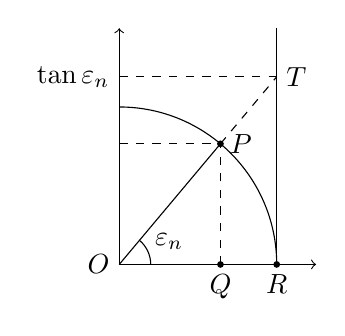
\begin{tikzpicture}[scale=2]
                \def\angle{50}

                \draw[->] (0,0) node[below, left] {\(O\)} -- (1.25,0);
                \draw[->] (0,0) -- (0,1.5);
                \draw (1,0) arc (0:90:1);
                \draw (0.2,0) arc (0:\angle:0.2);
                \node at (\angle*0.5:0.35) {\(\varepsilon_n\)};

                \draw[dashed] (0,{tan(\angle)}) -- (1,{tan(\angle)}) node[right] {\(T\)};
                \node[left] at (0, {tan(\angle)}) {\(\tan \varepsilon_n\)};

                \draw[-] (1,0) -- (1,1.5);
                
                \filldraw (\angle:1) circle (0.5pt);
                \draw[-] (0,0) -- (\angle:1) node[above, right] {\(P\)};
                \draw[dashed] (\angle:1) -- (\angle:{sqrt(1 + tan(\angle)*tan(\angle))});
                \draw[dashed] (0, {sin(\angle)}) -- ({cos(\angle)}, {sin(\angle)});

                \draw[dashed] ({cos(\angle)}, 0) -- (\angle:1);
                \filldraw ({cos(\angle)}, 0) node[below] {\(Q\)} circle (0.5pt);
                \filldraw (1, 0) node[below] {\(R\)} circle (0.5pt);
            \end{tikzpicture}
        \end{center}

        Per confronto di aree,
        l'area del triangolo \(OPQ\) è minore o uguale dell'area del settore circolare \(OPR\)
        che è minore o uguale del triangolo \(OTR\).
        
        Ricordiamo che l'area del settore circolare di angolo \(\alpha\) è data dalla proporzione
        \[
            \frac{\text{Area } S_\alpha}{\text{Area cerchio}} = \frac{\alpha}{2\pi}
        \]
        quindi
        \[
            \text{Area}_{OPR} = \frac{1}{2} \alpha
        \]
        Abbiamo allora che
        \[
            \frac{1}{2} \cos \varepsilon_n \sin \varepsilon_n
            \leq
            \frac{1}{2} \varepsilon_n
            \leq
            \frac{1}{2} \cdot 1 \cdot \tan \varepsilon_n
        \]
        che semplificando diventa
        \[
            \cos \varepsilon_n \leq \frac{\varepsilon_n}{\sin \varepsilon_n}
            \leq \frac{1}{\cos \varepsilon_n}
        \]
        Siccome \(\cos \varepsilon_n \to 1\) e \(\frac{1}{\cos \varepsilon_n} \to 1\),
        per il teorema dei carabinieri,
        \[
            \frac{\varepsilon_n}{\sin \varepsilon_n}
        \]
        Per la tangente abbiamo semplicemente
        \[
            \frac{\tan \varepsilon_n}{\varepsilon_n} = \left(\frac{\sin \varepsilon_n}{\varepsilon_n}\right)
            \left(\frac{1}{\cos \varepsilon_n}\right) \to 1
        \]
        E per il coseno abbiamo
        \begin{align*}
            \frac{1-\cos \varepsilon_n}{\varepsilon_n^2} &= \frac{
                (1 - \cos \varepsilon_n) ( 1 + \cos \varepsilon_n)
            }{
                \varepsilon_n^2 \cdot (1 + \cos \varepsilon_n)
            } \\
            &= \frac{1 - \cos^2 \varepsilon_n}{\varepsilon_n} \cdot \frac{1}{1 + \cos \varepsilon_n} \\
            &= {\left(\frac{\sin \varepsilon_n}{\varepsilon_n}\right)}^2 \left(\frac{1}{1 + \cos \varepsilon_n} \to \frac{1}{2}\right)
        \end{align*}
    \end{enumerate}
}

\sproposition{}{
    Calcolare il limite della successione
    \[
        a_n = (n+2)\sin\left(\frac{n+1}{n^2}\right)
    \]
    Notiamo che
    \[
        \varepsilon_n = \frac{n+1}{n^2} \to 0
    \]
    Scriviamo
    \begin{align*}
        a_n &= (n+2) \frac{\sin \varepsilon_n}{\varepsilon_n} \cdot \varepsilon_n \\
        &= \frac{\sin \varepsilon_n}{\varepsilon_n} \frac{(n+2)(n+1)}{n^2} \\
        &= \frac{\sin \varepsilon_n}{\varepsilon_n} \frac{n^2(1+\frac{2}{n})(1+\frac{1}{n})}{n^2}
        \to 1
    \end{align*}
}

\subsection{Proprietà asintotico}

\textbf{Nota:} non vale \(a_n \sim b_n \implies e^{a_n} \sim e^{b_n}\)
se \(a_n \to \infty\).
Per esempio, \(a_n = n + \sqrt{n} = n(1 + \frac{1}{\sqrt{n}}) \sim n = b_n\).
Quindi
\[
    \frac{e^{a_n}}{e^{b_n}} = e^{a_n-b_n} = e^{\sqrt{n}} \to +\infty
\]

\textbf{Nota:} non vale \(a_n \sim b_n \implies \log a_n \sim \log b_n\)
se \(a_n \to 1\).
Per esempio, \(a_n = 1 + \frac{1}{n}\) e \(b_n = 1 + \frac{1}{n^2}\).
Tuttavia,
\[
    \frac{\log a_n}{\log b_n} \to +\infty
\]

\textbf{Nota:} non vale \(a_n \sim b_n \land c_n \sim d_n \implies a_n \pm c_n \sim b_n \pm d_n\).
Per esempio, \(a_n = n + \sqrt{n} \sim n = b_n\).

\sproposition{Proprietà dell'o-piccolo}{
    \begin{itemize}
        \item Se \(a_n = o(b_n)\), allora \(a_n = \mathcal{O}(b_n)\);
        \item Se \(a_n = o(b_n)\) e \(c_n = \mathcal{O}(d_n)\),
        allora \(a_nc_n = o(b_nd_n)\). Infatti,
        \[
            \left|\frac{a_nc_n}{b_nd_n}\right| = \left|\frac{a_n}{b_n}\right| \left|\frac{c_n}{d_n}\right| 
        \]
        che tendono entrambi a zero;
        \item Se \(a_n = o(b_n)\) e \(c_n = o(b_n)\), allora \(a_n + c_n = o(b_n)\).
        Infatti,
        \[
            \frac{a_n + c_n}{b_n} = \frac{a_n}{b_n} + \frac{c_n}{b_n}
        \]
        che tendono entrambi a zero. Possiamo anche scrivere \(o(b_n) + o(b_n) = o(b_n)\);
    \end{itemize}
}

\subsection{Esercizi}

\sexercise{}{
    \[
        a_n = \frac{
            \log \left(\frac{n^2 + 1}{n}\right) + 1
        }{
            \sqrt{n^3 + 1} + \log n
        }
    \]
}

\sexercise{}{
    \[
        a_n = \frac{
            n^{1/2} + \cos(1/n) + \log n
        }{
            {(n + \sqrt{n})}^2 - \sqrt{n}
        }
    \]
}

\sexercise{}{
    \[
        a_n = \log \left(
            1 + \sin \left(\frac{\sqrt{n}}{n^2 + \log n}\right)
        \right)
        \left(\sqrt[3]{n^6 + 1} - n^2\right)
    \]
}

\sexercise{}{
    \[
        a_n = {\left(\cos \frac{1}{\sqrt{n}}\right)}^{\frac{n^3 - \log n}{\sqrt{n^4 + n}}}
    \]
}

\pagebreak 

\section{Serie numeriche}

\sexercise{}{
    Sia \(\{b_n\}\) una successione e sia \(\{b_{n\pm k_0}\}\) la successione traslata di
    \(\pm k\).
    Dimostrare che \(\lim b_n\) esiste se e solo se \(\lim b_{n \pm k_0}\) esiste e che i limiti sono uguali.
    % TODOURGENT
}

\sexample{}{
    Considera
    \[
        \sum_{n=1}^\infty \frac{1}{4n^2 - 1}
    \]
    Allora
    \[
        \frac{1}{4n^2 - 1} = \frac{1}{(2n+1)(2n-1)} = \frac{1/2}{2n-1} - \frac{1/2}{2n+1}
    \]
    Quindi
    \begin{align*}
        \frac{1}{2} \sum_{n=1}^\infty \left(\frac{1}{2n-1} - \frac{1}{2n+1}\right) \to
        \frac{1}{2}  
    \end{align*}
}

\sproof{Serie geometrica per Induzione}{
    %TODOURGENT
}

\sexample{}{
    Calcolare
    \[
        \sum_{n=0}^\infty {\left(\frac{1}{10}\right)}^n
    \]
    La serie ha ragione \(q = \frac{1}{10}\)
    e quindi
    \[
        \frac{1}{1 - \frac{1}{10}} = \frac{10}{9}
    \]
}

\sexercise{}{
    Calcolare
    \begin{align*}
        \sum_{n=1}^\infty \frac{3^n + 2\cdot 5^{n+1}}{7^{n+2}}
        &= \sum_{n=1}^\infty \frac{3^{n}}{7^{n+2}}
        + 2 \sum_{n=1}^\infty \frac{5^{n+1}}{7^{n+2}} \\
        &= \frac{1}{7^2} \sum_{n=1}^\infty \frac{3^{n}}{7^n}
        + \frac{2}{7} \sum_{n=1}^\infty \frac{5^{n+1}}{7^{n+1}} \\
        &= \frac{1}{7^2} \sum_{n=0}^\infty {\left(\frac{3}{7}\right)}^{n+1}
        +  \frac{2}{7} \sum_{n=0}^\infty {\left(\frac{3}{7}\right)}^{n+2} \\
        &= \cdots
    \end{align*}
}

\subsection{Aritmetica delle serie}

Le operazioni aritmetiche sulle serie sono giustificate a posteriori;
se alla fine vi è una forma di indecisione non erano legali.

\sproposition{}{
    Un numero decimale può essere espresso come
    \[
        x = N + \sum_{k=1}^\infty a_k \cdot 10^{-k}
    \]
}

\sexample{}{
    Mostriamo che se
    \(x = N, a_1 a_2 \cdots a_k \overline{9}\) dove \(a_j \in \{0,1,2,3,4,5,6,7,8,9\}\)
    e \(a_k < 9\),
    allora \(x = N a_1 a_2 \cdots (a_k + 1)\).
    Abbiamo quindi che
    \begin{align*}
        x &= N + \left( \sum_{j=1}^k a_j \cdot 10^{-j} \right)
        + \sum_{j=k+1}^\infty 9 \cdot 10^{-j} \\
        &= N + \left( \sum_{j=1}^{k-1} a_j \cdot 10^{-j} \right)
        + a_k \cdot 10^{-k} + 9\cdot 10^{-k-1}
        \sum_{h=0}^\infty 10^{-h} \\
        &= N + \left( \sum_{j=1}^{k-1} a_j \cdot 10^{-j} \right)
        + a_k \cdot 10^{-k} + 9 \cdot 10^{-k-1} \cdot \frac{10}{9} \\
        &= N + \left( \sum_{j=1}^{k-1} a_j \cdot 10^{-j}\right) + 10^{-k}(a_k + 1)
    \end{align*}
    Ciò può essere esteso ad ogni base.
}

\scorollary{}{
    Se \(a_n = o(b_n)\) cioè
    \[
        \frac{a_n}{b_n} \to 0
    \]
    per definizione di limite, fissato \(\varepsilon = 1\),
    esiste \(n_0\) tale che \(0 < \frac{a_n}{b_n} < 1 \implies 0 \leq a_n \leq b_n\)
    e quindi si applica il confronto.
}

\sexercise{}{
    Stabilire il carattere della serie
    \[
        \sum_{n=1}^\infty \frac{n^2 + {(1 + 1/n)}^n + \sin n}{{(n+\sqrt{n})}^3 + \log \left(\frac{n}{n+1}\right)}
    \]
    Notiamo che \(\forall n \geq 1, a_n \geq 0\).
    Notiamo allora che
    \[
        a_n = \frac{n^2 \left(1 + \frac{1}{n^2}{\left(1 + \frac{1}{n}\right)}^n + \frac{\sin n}{n}\right)}
        {n^3 \left\{{\left(1 + \frac{1}{\sqrt{n}}\right)}^3 + \frac{1}{n^3}\log\left(\frac{n}{n+1}\right)\right\}}
        \sim \frac{1}{n}
    \]
    Siccome la serie armonica è una serie-p con \(p=1\), allora la serie diverge.
}

\sexample{Teorema di condensazione}{
    È possibile applicare il teorema di condensazione alla serie armonica
    e ottenere che
    \[
        \sum_{k=0}^\infty {\left(\frac{1}{2^{p-1}}\right)}^k
    \]
    che è una serie geometrica di ragione
    \(\frac{1}{2^{p-1}}\) che converge se e solo se \(p>1\).
}

\stheorem{Rapporto di radici}{
    Sia \(\sum a_n\) una serie a termini \(\geq 0\) e supponiamo che
    una delle due condizioni sia soddisfatta:
    \begin{enumerate}
        \item \(\exists\, \underset{n}{\lim}\, \sqrt[n]{a_n} = L \in [0; +\infty]\);
        \item \(a_n > 0\) definitivamente e
            \(\exists\, \underset{n}{\lim}\, \frac{a_{n+1}}{a_n} = h \in [0; +\infty]\);
    \end{enumerate}
    Allora se \(L < 1\) la serie converge, mentre se \(L > 1\) allora
    \(a_n \to \infty\).
}

Se \(L=1\) il test è \textbf{inclonclusivo}.

La condizione della radice è più potente in quanto implica anche l'altra.

Infatti, con la p-serie armonica il limite tende a \(1\), il che coincide
con il fatto che la serie converge se \(p > 1\) e diverge altrimenti.

\scorollary{}{
    Sia \(\{a_n\}\) una successione con \(a_n \geq 0\).
    Se
    \[
        \exists\, \underset{n}{\lim}\, \sqrt[n]{a_n} = L
    \]
    oppure se il limite esiste e \(a_n \neq 0\) definitivamente,
    allora se \(L<1\), la serie converge e \(a_n \to 0\)
    e se \(L>1\) allora \(a_n \to +\infty\).
}

\sproof{}{
    Consideriamo il primo caso cosicché
    \[
        \exists\, \underset{n}{\lim}\, \sqrt[n]{a_n} = L
    \]
    Per definizione di limite, \(\forall \varepsilon > 0\) fissato
    \(\exists\, N\) tale che
    \[
        L-\varepsilon < \sqrt[n]{a_n} < L + \varepsilon
    \]
    Se \(L < 1\), esiste \(\varepsilon > 0\) tale che
    \(L+\varepsilon < 1\) (basta scegliere \(\varepsilon = (1-L)/2\)).
    Dalla disequazione \(\sqrt[n]{a_n} < L + \varepsilon\) deduciamo che
    \[
        \forall n \geq N, 0 \leq a_n < {(L+\varepsilon)}^n
    \]
    e poiché \(L+\varepsilon<1\) la serie converge per confronto
    con la serie geometrica
    \[
        \sum^\infty {(L+\varepsilon)}^n
    \]
    Se \(L > 1\) allora esiste \(\varepsilon > 0\)
    tale che \(L - \varepsilon > 1\), come per esempio
    \(\varepsilon = \frac{L-1}{2}\), quindi per \(n\geq N\) abbiamo
    \[
        \sqrt[n]{a_n} > (L - \varepsilon) > 1
    \]
    elevando alla \(n\) otteniamo \(a_n > {(L-\varepsilon)}^n \to +\infty\)
    e per confronto \(a_n \to +\infty\).
    In particolare, \(a_n\) non tende a zero e la serie diverge per il criterio
    del termine ennesimo.

    Per il secondo caso, \(\exists\, \underset{n}{\lim}\, \frac{a_{n+1}{a_n}} = L\)
    come nel caso precedente. Quindi \(\forall \varepsilon > 0\)
    esiste \(N\) tale che 
    \[
        L - \varepsilon < \frac{a_{n+1}}{a_n} < L + \varepsilon
    \]
    Sappiamo per esempio che \(L > 1\) cosicché come nel caso precedente
    possiamo scegliere \(\varepsilon\) tale che
    \(L - \varepsilon > 1\) e abbiamo che \(\forall n \geq N\)
    \[
        \frac{a_{n+1}}{a_n} > L - \varepsilon > 1 > 0
    \]
    \(\forall n \geq N\) moltiplicando i termini membro a membro
    \[
        \frac{a_{N+1}}{a_N} \cdot
        \frac{a_{N+2}}{a_{N+1}} \cdot
        \frac{a_{N+3}}{a_{N+2}} \cdots
        \frac{a_{n}}{a_{n-1}} \cdot
        \frac{a_{n+1}}{a_{N}}
        = \frac{a_{n+1}}{a_{N}} \geq {(L-\varepsilon)}^{n-N+1}
    \]
    Ciascuno di questi è più grande di \(L - \varepsilon\).
    Quindi,
    \[
        a_{n+1} \geq {(L-\varepsilon)}^{-N+1}
        \cdot
        {(L-\varepsilon)}^n \cdot a_N \to +\infty
    \]
    e per confronto \(a_n \to +\infty\).
}

\sexample{}{
    Consider
    \[
        \sum_{n=1}^\infty \frac{A^n}{n!}
    \]
    con \(A > 0\).
    Quando ci sono i fattoriali usiamo il criterio dei rapporti.
    Abbiamo che
    \[
        \forall n, a_n = \frac{A^n}{n!} > 0
    \]
    per il criterio del rapporto
    \begin{align*}
        \frac{a_{n+1}}{a_n} = \frac{A^n}{(n+1)!}
        \cdot \frac{n!}{A^n} = \frac{A}{n+1} \to 0
    \end{align*}
    Quindi la serie converge, e converge a \(e^A - 1\).
}

\sexample{}{
    Consider
    \[
        \sum_{n=1}^\infty \frac{e^{n^2} + {(\log n)}^n + {\left(1 + \frac{1}{n}\right)}^n}{n^n + e^{3n\log n} + {\left(n+\frac{1}{n}\right)}^{17}}
    \]
    che è ovviamente positivo.
    Usiamo il criterio asintotito.
    A numeratore l'ultimo termine è finito e tende ad \(e\).
    Dobbiamo verificare quale degli altri due termini è dominante.
    Scriviamo allora \({(\log n)}^n = e^{n\log\log n}\).
    Allora chiaramente \(e^{n^2}\) domincia sull'altro termine.
    Analogamente, a denominatore abbiamo \(n^n = e^{n\log n}\)
    come termine dominante.
    \[
        a_n =  \frac{
            e^{n^2} \left\{
            1 + e^{n\log \log(n) - n^2}
            + {\left(1 + \frac{1}{n}\right)}^{n} \cdot e^{-n^2}
        \right\}
        }{
            e^{3n\log n} \left\{
                1 + e^{-2n\log n} + {\left(1 + \frac{1}{n}\right)}^{17}
                \cdot e^{-3n\log n}
            \right\}
        } \sim \frac{e^{n^2}}{e^{3n\log n}}
    \]
    Allora
    \[
        e^{n\log \log n - n^2} = e^{-n^2 \left\{1 - \frac{\log\log n}{n^2}\right\}}
        \to \infty
    \]
    quindi la serie diverge.
    Oppure, con il criterio della radice
    \[
        {\left(e^{n^2 - 3n \log n}\right)}^{\frac{1}{n}}
        = e^{n\left(1 - \frac{3\log n}{n}\right)} \to \infty > 1
    \]
}

\sexample{}{
    Studiare il carattere di
    \[
        \sum^\infty \frac{
            n^{n\log n}
        }{
            (2n)!
        }
    \]
    che ha termini positivi. Ci sono dei fattoriali quindi conviene utilizzare il criterio
    del rapporto.
    Notiamo che \((2n+2)! = (2n+2)(2n+2)(2n)!\)
    e \((n+1)\log(n+1) = n\log(n+1) + \log(n+1) = n[\log n + \log(1 + 1/n)] + \log(n+1)\).
    Il rapporto è dato da\begin{align*}
        \frac{a_{n+1}}{a_n} &= \frac{
            {(n+1)}^{(n+1)\log(n+1)}
        }{
            (2n+2)!
        }
        \cdot
        \frac{
            (2n)!
        }{
            n^{n\log n}
        } \\
        &= \frac{
            {(n+1)}^{n\log n} \cdot {(n+1)}^{n\log(1 + 1/n) + \log(n+1)}
        }{
            n^{n\log n}
        }
    \end{align*}
    Con
    \[
        {\left(1 + \frac{1}{n}\right)}^{n\log n}
        \cdot {(n+1)}^{n\log(1 + 1/n)}
        \cdot {(n+1)}^{\log (n+1)}
    \]
    troviamo
    \[
        \frac{1}{((2n+2)(2n+1))} \cdot {\left[
            {\left(1 + \frac{1}{n}\right)}^n
        \right]}^{\log n}
        \cdot {(n+1)}^{n\log (1 + 1/n)}{(n+1)}^{\log(n+1)}
    \]
    Dal primo e ultimo termine possiamo notare che la serie va ad infinito.
}

\sexample{}{
    Considera
    \[
        \sum_{n=1}^\infty
        \frac{
            2^{\sqrt{n}}
        }{
            n^{\log n}
        }
    \]
    Il criterio della radice non funziona. Infatti,
    \begin{align*}
        \sqrt[n]{a_n}
        = \frac{
            2^{1 / \sqrt{n}}
        }{
            n^{\frac{\log n}{n}}
        }
    \end{align*}
    Il numeratore tende a \(1\),
    mentre scriviamo il denominatore come
    \begin{align*}
        n^{\frac{\log n}{n}} &=
        e^{\frac{1}{n}\log \left(n^{\log n}\right)} \\
        &= e^{\frac{1}{2}{\left(\log n\right)}^2} \to 1
    \end{align*}
    Allora il limite è \(L=1\), quindi il criterio è inconclusivo.
    Allora
    \begin{align*}
        a_n &= \frac{
            a^{\sqrt{n}\log 2}
        }{
            e^{{(\log n)}^2}
        } \\
        &= e^{\sqrt{n} \log 2 - {\left(\log n\right)}^2} \\
        &= e^{\sqrt{n} \left\{\log 2 - \frac{{\log n}^2}{\sqrt{n}}\right\}}
    \end{align*}
    L'esponente tende a infinito quindi la serie diverge per il criterio
    del termine n-esimo.
}

\sexample{}{
    \[
        \sum_{n=1}^\infty
        \frac{
            n^{\log n}
        }{
            2^{\sqrt{n}}
        }
    \]
    che ha i termini della serie precedente ma invertiti.
    Dobbiamo usare il confronto per mostrare che la serie converge.
    Confrontiamo la serie con una p-serie, per esempio \(\sum\frac{1}{n^2}\).
    Il rapporto è dato da
    \begin{align*}
        \frac{a_n}{\frac{1}{n^2}}
        &= n^2 a_n  \\
        &= e^{2\log n - \sqrt{n}\left\{\log 2 - \frac{{(\log n)}^2}{\sqrt{n}}\right\}}
    \end{align*}
    e abbiamo che
    \begin{align*}
        2\log n - \sqrt{n}\log 2 + {(\log n)}^2
        = -\sqrt{n} \left\{
            \log 2 - \frac{2\log n}{\sqrt{n}}
            - \frac{{(\log n)}^2}{\sqrt{n}} \to -\infty
        \right\}
    \end{align*}
    e quindi il rapporto tende a \(0\). Quindi,
    il rapporto è minore di 1 definitivamente
    e la serie converge per confronto.
}

\subsection{Formula di Stirling}

\sexample{}{
    Studia il carattere di
    \[
        \sum_{n=1}^\infty \frac{n^n}{(2n)!}
    \]
    Il limite è dato da
    \begin{align*}
        \frac{a_{n+1}}{a_n} = \frac{
            {(n+1)}^{n+1}
        }{
            (2n+2)!
        }
        \cdot
        \frac{
            (2n)!
        }{
            n^n
        }
        &=
        {\left(\frac{n+1}{n}\right)}^n
        \frac{
            (n+1)(2n)!
        }{
            (2n+2)(2n+1)(2n)!
        } \\
        &=
        {\left(\frac{n+1}{n}\right)}^n
        \frac{n+1}{(2n+2)(2n)!}
        \sim e \cdot  \frac{
            n+1
        }{
            (2n+2)(2n+1)
        } \\
        &= \frac{e^{n(1+1/n)}}{{(2n)}^2 {\left(1 + \frac{1}{n}\right)}{\left(1 + \frac{1}{2n}\right)}}
        \to 0
    \end{align*}
    Quindi la serie converge.

    Con radici abbiamo
    \begin{align*}
        {\left[\frac{n^n}{(2n)!}\right]}^{1/n}
        &= \frac{n}{
            {\left[
                {(2n)}^{2n}
                \cdot 2^{-2n} \cdot \sqrt{4\pi n}(1 + o(1))
            \right]}^{1/n}
        } \\
        &= \frac{n}{
            {(2n)}^2 \cdot e^{-2} {(4\pi)}^{\frac{1}{2n}}
            \cdot n^{\frac{1}{2n}}{(1 + o(1))}^{\frac{1}{n}}
        } \to 0
    \end{align*}
    E quindi converge
}

\sexample{}{
    Studia il carattere di
    \[
        \sum_{n=1}^\infty \frac{e^{n^2} + n^n}{(n^2)! + {\left(1 + \frac{1}{n}\right)}^{n^2}}
    \]
    A numeratore abbiamo
    \begin{align*}
        e^{n^2} + n^n = e^{n^2} + e^{n \log n} = e^{n^2}
        \left\{1 + e^{n\log n - n^2}\right\}
        \sim e^{n^2}
    \end{align*}
    A denominatore abbiamo
    \begin{align*}
        (n^2)! + {\left(1 + \frac{1}{n}\right)}^{n^2}
        &= {(n^2)}^{n^2} \cdot e^{-n^2}
        \cdot \sqrt{2\pi n^2}(1 + o(1))
        + e^{n^2 \log \left(1 + \frac{1}{n}\right)} \\
        &= e^{2n^2 \left\{
            \log n - \frac{1}{2} + \frac{1}{2n^2} \log \sqrt{2\pi n^2}
        \right\}}(1 + o(1)) + e^{n^2 \log\left(1 + \frac{1}{n}\right)}
        \\
        &= e^{2n^2 \left\{
            \log n - \frac{1}{2} + \frac{1}{2n^2} \log\sqrt{2\pi n^2}
        \right\}}
        \left\{1 + o(1) + e^{n^2\log\left(1 + \frac{1}{n}\right) - 2n^2 \left\{\cdots\right\}}\right\} \\
        &\sim e^{2n^2 \left\{
            \log n - \frac{1}{n} + \frac{1}{2n^2}
            \log\sqrt{2\pi n^2}
        \right\}}
        = {(n^2)}^{n^2} e^{-n^2} \sqrt{2\pi n^2}
    \end{align*}
    Ora possiamo usare il criterio della radice
    \begin{align*}
        a_n \sim \frac{
            e^{n^2}
        }{
            {(n^2)}^{n^2}
            e^{-n^2}
            \sqrt{2\pi n^2}
        }
        = b_n
    \end{align*}
    Abbiamo che \(\sum a_n\) ha lo stesso carattere di \(\sum b_n\)
    e
    \begin{align*}
        \sqrt[n]{b_n} &= \frac{
            e^n
        }{
            {(n^2)}^n e^{-n}
            {(2n)}^{\frac{1}{2n}} n^{1/n}
        } \\
        &= \frac{
            e^{2n}
        }{
            n^{2n} {(2n)}^{1/n} n^{1/n}
        } \to
        0
    \end{align*}
    e quindi la serie converge.
}

\pagebreak

\subsection{Serie a termini di segno qualunque}

Con serie di segno qualunque non è possibile applicare il criterio asintotico.

Sia \(\{a_n\}\) una successione reale o complessa (o in uno spazio metrico)
e supponiamo che esista finito il limite \(\underset{n}{\lim}\, a_n = L \in \mathbb{F}\).
Per definizione di limite, \[\forall \varepsilon > 0, \exists\, N \,|\, \forall n \geq N,
|a_n - L| < \varepsilon\]
Quindi, se \(n,m > N\), allora
\[
    |a_n - a_m| = |(a_n - L) + (L - a_m)|
    \trianglelefteqslant
    |a_n - L| + |L - a_m|
    < 2 \varepsilon
\]

\sdefinition{Successione di Cauchy}{
    Sia \(\{a_n\}\) una successione reale o complessa.
    Si dice che \(\{a_n\}\) soddisfa la condizione (C) di Cauchy, o più brevemente
    che è una successione di Cauchy,
    se
    \[
        \forall \varepsilon > 0, \exists\, n \,|\,
        \forall n,m \geq M,
        |a_n - a_m| < \varepsilon
    \]
    Per quanto visto sopra, se \(a_n \to L\) finito, allora \(\{a_n\}\)
    è di Cauchy.
}

\stheorem{}{
    Sia \(\{a_n\}\) una successione reale o complessa.
    Sono equivalenti:
    \begin{enumerate}
        \item \(\exists\) finito
        \[
            \underset{n}{\lim}\, a_n = L
        \]
        \item \(\{a_n\}\) è una successione di Cauchy.
    \end{enumerate}
}

Abbiamo visto che (1) implica (2). Il converso, vale in \(\mathbb{R}\)
ma non in \(\mathbb{Q}\).

\sproposition{}{
    Sia
    \[
        \sum^\infty a_n
    \]
    una serie reali o complessa e sia \(\{S_N\}\)
    la successione delle sue somme parziali.
    Per definizione, \(\sum a_n\) converge a \(S\) se esiste
    finito \(\underset{n}{\lim}\, S_n \in \mathbb{R}\).
}

\scorollary{}{
    Condizione necessaria e sufficiente perché una serie \(\sum a_n\) converga
    e che la successione delle somme parziali soddisfi le condizioni di Cauchy, scritte
    in 3 modi equivalenti:
    \begin{enumerate}
        \item \[ \forall \varepsilon > 0, \exists\, N \,|\, \forall n,m \geq N, |S_N - S_M| < \varepsilon\]
        equivalentmeente notando che se \(n>m\), \[S_n - S_m = \sum_{k=1}^n a_k - \sum_{k=1}^m a_k = \sum_{m+1}^{n} a_k\]
        \item \[
            \forall \varepsilon > 0, \exists\, N \,|\, \forall n,m \geq N
            \quad n>m \quad \left|\sum_{k=m+1}^n a_k\right| < \varepsilon
        \]
        ovvero
        \[
            \forall \varepsilon > 0, \exists\, N \,|\, \forall n,m \geq N
            \quad n\geq m \quad \left|\sum_{k=m+1}^n a_k\right| < \varepsilon
        \]
        \item \textbf{condizione più usata:}
        \[
            \forall \varepsilon > 0, \exists\, N \,|\,
            \forall m,n \geq N \land \forall p \geq 0, \left|\sum_{k=m}^{m+p} a_k\right|
            < \varepsilon
        \]
    \end{enumerate}
}

La serie
\[
    \sum_{n=1}^\infty \frac{{(-1)}^n}{n^p}
\]
con \(0 < p \leq 1\) converge ma non assolutamente.
La serie converge per \(p > 0\).

\slemma{disuguaglianza triangolare generalizzata}{
    Sia \(\{b_k\}\) una successione,
    allora
    \[
        \left|\sum_{k=1}^n b_k\right|
        \leq
        \sum_{k=1}^n |b_k|
    \]
}

\sproof{}{
    Per induzione
    \begin{itemize}
        \item il caso base è banale;
        \item \begin{align*}
            \left|
                \sum_{k=1}^{n + 1} b_k
            \right|
            &= \left|
                \left(
                    \sum_{k=1}^{n} b_k
                \right)
                + b_{n+1}
            \right|
            \trianglelefteqslant \left|
                \sum_{k=1}^{n} b_k
            \right|
            + |b_{n+1}| \\
            &= \sum_{k=1}^{n} |b_k|
            + |b_{n+1}| = \sum_{k=1}^{n+1} |b_k|
        \end{align*}
    \end{itemize}
}

\sproof{Teorema fondamentale}{
    Sapendo che
    \[
        \sum_{k=1}^\infty |a_k| < +\infty
    \]
    la tesi è che
    \[
        \sum_{k=1}^\infty a_k
    \]
    converga equivalentemente soddisfa le condizionid i Cauchy.
    \[
        \forall \varepsilon > 0, \exists\, N \,|\,
        \forall n \geq m \geq N, \left|\sum_{k=m}^n a_k\right| \leq \varepsilon
    \]
    Per ipotesi \(\sum |a_k|\) converge quindi soddisfa la condizione di Cauchy
    e dato \(\varepsilon > 0\), esiste \(N\) tale che \(\forall n \geq m \geq N\)
    \[
    \left|
        \sum_{k=m}^n |a_k|
    \right|
    = \sum_{k=m}^n |a_k| \varepsilon
    \]
    Ma per il lemma \(\forall n \geq m \geq N\),
    \[
        \left|
        \sum_{k=m}^n a_k
        \right|
        \leq \sum_{k=m}^n |a_k| < \varepsilon
    \]
}

Quando abbiamo una serie che non ha termini solo positivi, la prima cosa da fare
è mettere il modulo e controllare la convergenza assoluta.

\sexample{}{
    Considera
    \[
        \sum \frac{\sin n}{n^2}
    \]
    che non ha termini solo positivi. Allora proviamo a studiare la convergenza assoluta.
    \[
        \sum \frac{|\sin n|}{n^2}
    \]
    Poiché \(\frac{|\sin n|}{n^2} \leq \frac{1}{n^2}\)
    e \(\sum \frac{1}{n^2 \leq +\infty}\)
    converge (p-serie), allora la serie dei moduli converge assolutamente e quindi converge.
}

Vale lo stesso procedimento per
\[
    \sum \frac{\sin n}{n^p}
\]
con \(p > 1\).
Se \(p \leq 1\), allora diverge. Ciò segue dal fatto che, per esempio,
\(|\sin x| > \frac{1}{2}\) se \(\frac{\pi}{6} + k\pi \leq x \leq \frac{5}{6}\pi + k\pi\)
con \(k\in\mathbb{Z}\). Notiamo che l'intervallo
\[
    I_k = \left[\frac{\pi}{6} + k\pi; \frac{5}{6}\pi + k\pi\right]
\]
ha lunghezza \(\frac{2\pi}{3} > 1\), quindi conviene un interno \(n\),
in realtà \(2\) interi in quando la lunghezza è maggiore di \(2\).
Allora la serie \[
    \sum \frac{|\sin n|}{n}
    \geq 
    \sum_{k\in\mathbb{N}} \frac{|\sin n_k|}{n_k}
\]
dove \(n_k\) è un intero in ognuno di \(I_k\).
Ciò è maggiore o uguale di
\[
    \sum \frac{\frac{1}{2}}{\frac{5}{6} \pi + k\pi}
\]
in quanto il valore a denominatore è al minomo \(\frac{5}{6} \pi + k\pi\).
Allora troviamo un multiplo della serie armonica, che diverge.

\sexample{}{
    Considera
    \[
        \sum \frac{
            -n + {(\sin n)}n^2 - \log n
        }{
            {(1+n)}^{10/3} - \cos n
        }
    \]
    allora guardiamo il modulo:
    \[
        |a_n| = \frac{
            |-n + (\sin n)n^2 - \log n|
        }{
            |{(1+n)}^{10/3} - \cos n|
        }
    \]
    Maggioriamo rendendo più piccolo il denominatore e più grande il numeratore.
    \[
        |a_n| \leq \frac{
            n + n^2|\sin n| + |\log n|
        }{
            {(1+n)}^{10/3} -1
        }
    \]
    Notiamo che \({(1+n)}^{10/3} - 1 \geq \frac{1}{2}{(1+n)}^{10/3} > \frac{1}{2}n^{10/3}\)
    perché \(n=1\) dà il valore massimo. Quindi
    \[
        |a_n| \leq \frac{
           n
        }{
            \frac{1}{2}n^{10/3}         
        }
        + \frac{n^2}{\frac{1}{2}n^{10/3}}
        + \frac{\log n}{\frac{1}{2}n^{10/3}}
    \]
    Quindi
    \[
        \sum_{n=1}^\infty |a_n| \leq
        2 \sum n^{-\frac{7}{8}}
        +
        2 \sum n^{-\frac{4}{3}}
        + 2 \sum_{n=2} \frac{1}{n^{10/3} {(\log n)}^{-1}}
    \]
    Tutti i termini convergono e quindi la serie converge.
}

Perché il teorema valga basta che \(a_n \geq 0\) e \(a_n \geq a_{n+1}\)
valgano definitivamente.
In tal caso la stima dell'errore vale solo per \(n\) sufficientemente grande.

\sexample{}{
    Si può applicare il teorema a
    \[
        \sum_{n=1}^\infty \frac{{(-1)}^n}{n^p}
    \]
    e notare che la serie converge semplicemente ma non assolutamente per ogni \(0 < p \leq 1\).
}

\pagebreak

\sexample{}{
    Considera
    \[
        \sum_{n=1}^\infty {(-1)}^n a_n
    \]
    con
    \[
        a_n = \begin{cases}
            \frac{1}{n^2} & n \text{ pari} \\
            \frac{1}{n^4} & n \text{ dispari}
        \end{cases}
    \]
    Poiché \(\forall n \geq 1\), \(a_n \leq \frac{1}{n^2}\) e quindi \(p = 2 > 1\) e quindi la serie converge assolutamente,
    e quindi converge. Tuttavia, è chiaro che \(\forall n, a_{2n+1} < a_{2n+2}\).
}

\textbf{Nota:}
\(a_n \sim b_n\) e \(b_n\) monotona crescente non implica necessariamente che \(a_n\) sia monotona
decrescente.

Infatti,
\sexample{}{
    Consideriamo
    \[
        a_n = \frac{1}{\sqrt{n}} + {(-1)}^n \frac{1}{n}
    \]
    e \(b_n = \frac{1}{\sqrt{n}}\).
    È chiaro che \(b_n\) è strettamente monotona decrescente.
    Inoltre, \[
        a_n = \frac{1}{\sqrt{n}} \left\{
            1 + {(-1)}^n \frac{1}{\sqrt{n}}
        \right\} \sim
        \frac{1}{\sqrt{n}} = b_n
    \]
    Verifichiamo allora che
    \[
        a_{2k} > a_{2k-1}
    \]
    Infatti, \(a_n\) non può essere definitivamente monotona decrescente in quanto
    se \(a_n\) fosse definitivamente monotona decrescente, allora la serie
    \[
        \sum_{n=1}^\infty {(-1)}^n a_n
    \]
    per il teorema di Leibniz sarebbe convergente.
    Tuttavia,
    \begin{align*}
        \sum_{n=1}^\infty {(-1)}^n \left\{
            \frac{1}{\sqrt{n}} + {(-1)}^n \frac{1}{n}
        \right\}
        &=  \sum_{n=1}^\infty \left\{
            {(-1)}^n \frac{1}{\sqrt{n}} + \frac{1}{n}
        \right\} \\
        &= \sum_{n=1}^\infty \left( {(-1)}^n \frac{1}{\sqrt{n}} \right)
        + \sum_{n=1}^\infty \left( \frac{1}{\sqrt{n}} \right)
    \end{align*}
    dove il secondo addendo chiaramente diverge.
    Allora, la serie di partenza diverge, nonostante il primo addendo converga.
}

\pagebreak

\sexample{Stima errore teorema Leibniz}{
    Calcolare la somma della serie
    \[
        \sum_{n=0}^\infty \frac{{(-1)}^n}{n!} = e^{-1}
    \]
    con un errore minore di \(10^{-3}\).
    Abbiamo allora
    \[
        a_n = \frac{1}{n!}
    \]
    e \[
        \frac{a_{n+1}}{a_n} = \frac{1}{n+1} \to 0
    \]
    La serie converge assolutamente per il criterio della radice e per il criterio del rapporto.
    La serie è a termini alterni, \(a_n \to 0\) e \(a_{n+1} < a_n\), quindi vale la condizione per il teorema di Leibniz.
    Per l'errore abbiamo
    \[
        \forall N, |E_N| = |S - S_n| < \frac{1}{(N+1)!}
    \]
    Se noi imponiamo che \(\frac{1}{(N+1)!} < 10^{-3}\) certamente \(|E_N| < 10^{-3}\).
    Dobbiamo usare almeno \(N=6\) per ottenere \((N+1)!=5040 > 1000\).
    Allora,
    \[
        \sum_{n=0}^\infty \frac{{(-1)}^n}{n!} = 1 - \frac{1}{1} + \frac{1}{2!} - \frac{1}{3!}
        \cdots + \frac{1}{6!} = S_6
    \]
    che ha un errore minore o uguale di \(\frac{1}{6!}\).
}

\sexample{}{
    Studiare
    \[
        \sum_{n=1}^\infty {(-1)}^n \frac{\sqrt{n}}{n+1}
    \]
    la serie ha termini alterni con \(a_n = \frac{\sqrt{n}}{n+1}\).
    Controlliamo la convergenza assoluta:
    \begin{align*}
        a_n = \frac{1}{\sqrt{n}} \frac{1}{(1+1/n)} \sim \frac{1}{n^{1/2}}
    \end{align*}
    e
    \[
        \sum \frac{1}{n^{1/2}} = +\infty
    \]
    in quanto \(p = \frac{1}{2} \leq 1\) e quindi non converge assolutamente.
    Vogliamo ora usare il teorema di Leibniz.
    Le condizioni sono soddisfatte in quanto \(a_n \geq 0\) e \(a_n \sim \frac{1}{\sqrt{n}}\).
    Verifichiamo esplicitamente
    \begin{align*}
        a_n - a_{n+1} &= \frac{\sqrt{n}}{n+1} - \frac{\sqrt{n-1}}{n+2} \\
        &= \frac{\sqrt{n}(n+1)-{(n+1)}^{3/2}}{(n+1)(n+2)}
    \end{align*}
    Studiamo allora quando il numeratore è maggiore di zero.
    \begin{align*}
        \sqrt{n}(n+2) \geq {(n+1)}^{3/2}
    \end{align*}
    Siccome i termini sono tutti positivi, possiamo fare il quadrato
    \begin{align*}
        n{(n+2)}^2 \geq {(n+1)}^3 &= n^3 + 4n^2 + 4n \\
        & \geq n^3 + 3n^2 + 3n + 1
    \end{align*}
    che è sempre vero.
    Alternativamente, potremmo fare il limite con \(n \to \infty\) del numeratore
    \begin{align*}
        \sqrt{n}(n+2) - {(n+1)}^{3/2} &= n^{3/2} \left\{
            1 - \frac{2}{n} - {\left(1 + \frac{1}{n}\right)}^{3/2}
        \right\}
    \end{align*}
    Abbiamo che
    \begin{align*}
        \frac{2}{n} + 1- \left(1 + \frac{1}{n}\right)^{3/2} &= \frac{2}{n} - \left\{
            {\left(1+\frac{1}{n}\right)}^{3/2} - 1
        \right\}
    \end{align*}
    e
    \begin{align*}
        {\left(1+\frac{1}{n}\right)}^{3/2} - 1 \sim {(1+\varepsilon_n)}^{\alpha} - 1
        \sim \alpha \varepsilon_n
    \end{align*}
    e quindi
    \begin{align*}
        \frac{2}{n} - \left\{
            {\left(1+\frac{1}{n}\right)}^{3/2} - 1
        \right\}
        &= \frac{2}{n} - \frac{3}{2}\frac{1}{n} (1 + o(1)) \\
        &= \frac{1}{2n} - \frac{3}{2}\frac{1}{n}o(1) \\
        &= \frac{1}{2n} + \frac{1}{n}o(1) \\
        &= \frac{1}{n} \left\{\frac{1}{2} + o(1)\right\} \\
        &\sim \frac{1}{2n}
    \end{align*}
    Adesso, per permanenza del segno, il fatto che il numeratore tenda ad infinito, implica che sia maggiore di zero
    definitivamente.
    Allora, possiamo utilizzare il teorema di Leibniz.
    Alternativamente, se non risuciamo a mostrare che i termini siano decrescente, abbiamo
    \[a_n = \frac{\sqrt{n}}{n+1} \sim \frac{1}{\sqrt{n}} = b_n\]
    e \(b_n\) è decrescente. Allora, scriviamo \[
        a_n = \frac{1}{\sqrt{n}} + \left(\sqrt{n}{n+1} - \frac{1}{\sqrt{n}}\right)
    \]
    Cosifacendo, abbiamo che
    \begin{align*}
        \sum_{n=1}^infty {(-1)}^n a_n &= \sum_{n=1}^\infty \left\{ {(-1)}^n \frac{1}{\sqrt{n}} + {(-1)}^n \left(
            \frac{\sqrt{\sqrt{n}}}{n+1} - \frac{1}{\sqrt{n}}
        \right)\right\} \\
        &= \sum_{n=1}^\infty {(-1)}^n \frac{1}{\sqrt{n}} + \sum_{n=1}^\infty {(-1)}^n
        \left(\frac{\sqrt{n}}{n+1} - \frac{1}{\sqrt{n}}\right)
    \end{align*}
    Se non ci sono forme di intedeterminazione nel membro di destra,
    \begin{align*}
        \sum^\infty {(-1)}^n \frac{1}{\sqrt{n}}
    \end{align*}
    converge semplicemente ma non assolutamente per il teorema di Leibniz.
    La seconda serie
    \begin{align*}
        \sum {(-1)}^n \left(
            \frac{\sqrt{n}}{n+1} - \frac{1}{\sqrt{n}}
        \right)
    \end{align*}
    ha modulo
    \begin{align*}
        \left| \frac{\sqrt{n}}{n+1} - \frac{1}{\sqrt{n}} \right| &= \frac{1}{\sqrt{n}} - \frac{\sqrt{n}}{n+1} \\
            &= \frac{(n+1) - \sqrt{n}\sqrt{n}}{\sqrt{n}(n+1)} \\
            &= \frac{1}{\sqrt{n}(n+1)} \\
            &= \frac{1}{n^{3/2}(1 + 1/n)} \sim \frac{1}{n^{3/2}}
    \end{align*}
    Concludiamo quindi che
    \[
        \sum {(-1)}^n a_n
    \]
    converge come somma di
    \[
        \sum {(-1)}^n \frac{1}{\sqrt{n}}
    \]
    che converge semplicemente ma non assolutamente e
    \[
        \sum {(-1)}^n \left( \frac{\sqrt{n}}{n+1} - \frac{1}{\sqrt{n}} \right)
    \]
    che converge assolutamente e la convergenza non può essere assoluta perché
    se \(\sum a_n\) e \(\sum b_n\) convergano assolutamente allora \(\sum (a_n + b_n)\)
    converge assolutamente. Infatti,
    \[
        \sum |a_n - b_n| \leq \sum (|a_n| + |b_n|)
        = \sum |a_n| + \sum |b_n| < +\infty
    \]
}

\subsection{Serie con parametri}

\sexample{}{
    Considera
    \[
        \sum_{n=1}^\infty \frac{\log n}{n+1}{\left(x^2-x-2\right)}^2
    \]
    Controlliamo la positività
    \begin{align*}
        x^2 - x - 2 \geq 0
    \end{align*}
    per \(x \leq - 1 \lor x \geq 2\), altrimenti i termini sono alterni.
    Studiamo la convergenza assoluta usando il criterio di radice/rapporto
    \begin{align*}
        {\left|\frac{\log n}{n+1}(x^2 - x - 2)\right|}^{1/n}
        &= \frac{{\left(\log n\right)}^{1/n}}{{\left[n(1+1/n)\right]}^{1/n}}
    \end{align*}
    Scriviamo che \({\left(\log n\right)}^{1/n} = e^{\frac{1}{n}\log\log n} \to 1\)
    e \(n^{\frac{1}{n}} \to 1\) (limite notevole)
    e
    \[
        {\left(1 + \frac{1}{n}\right)}^{\frac{1}{n}} \to 1
    \]
    Quindi \(|x^2 - x - 2| = L\)
    e se \(L < 1\), la serie converge assolutamente, se \(L> 1\) il modulo del termine generale diverge e la serie non converge
    e diverge dove è a termini non-negativi.
    Dobbiamo allora risolvere la disequazione \(L<1\)
    \begin{align*}
        |x^2 - x - 2| < 1
    \end{align*}
    Siccome \(|t| < a \iff -a < t < a\) scriviamo che ciò è equivalente a
    \begin{align*}
        \begin{cases}
            x^2 - x - 2 < 1 \\
            x^2 - x - 2 > -1
        \end{cases}
        \equiv
        \begin{cases}
            x^2 - x - 3 < 0 \\
            x^2 - x - 1 > 0
        \end{cases}
    \end{align*}
    Le soluzioni della prima sono
    \[
        \frac{1-\sqrt{13}}{2} < x < \frac{1 + \sqrt{13}}{2}
    \]
    mentre della seconda
    \[
        x < \frac{1-\sqrt{5}}{2} \lor x > \frac{1 + \sqrt{5}}{2}
    \]
    Allora abbiamo che la serie converge assolutamente in \(\frac{1-\sqrt{13}}{2} < x < \frac{1 - \sqrt{5}}{2}\)
    e \(\frac{1 + \sqrt{5}}{2} < x < \frac{1+\sqrt{13}}{2}\).
    Se \(\frac{1-\sqrt{5}}{2} < x < \frac{1 + \sqrt{5}}{2}\), la serie non converge (presumibilmente oscilla ma bisognerebbe mostrarlo).
    Invece, se \(x < \frac{1 - \sqrt{3}}{2}\) oppure \(x > \frac{1 + \sqrt{13}}{2}\) la serie non converge ed è a termini positivi,
    quindi diverge necessariamente.
    Manca ancora il caso per cui \(L=1\).
    In tale caso, \(x = \frac{1 \pm \sqrt{5}}{2}\) oppure \(x = \frac{1 \pm \sqrt{13}}{2}\).
    Nel caso in cui \(x = \frac{1 \pm \sqrt{13}}{2}\) sappiamo che \(x^2 - x - 2 = 1\)
    e la serie diventa
    \[
        \sum_{n=1}^\infty \frac{\log n}{n+1}
    \]
    con
    \begin{align*}
        a_n = \frac{\log n}{n+1} = \frac{\log n}{n(1 + 1/n)} \sim \frac{\log n}{n}
        = \frac{1}{n{(\log n)}^{-1}}
    \end{align*}
    che è quindi una p-q serie con \(p=1\) e \(q > 1\), quindi la serie diverge.
    Invece, se \(x = \frac{1 \pm \sqrt{5}}{2}\) abbiamo che \(x^2 - x - 2 = -1\)
    e la serie diventa
    \[
        \sum_{n=1}^\infty {(-1)}^n \frac{\log n}{n+1}
    \]
    che non converge assolutamente (caso di prima). Tuttavia,
    \begin{align*}
        a_n &= \frac{\log n}{n+1} \sim \frac{\log n}{n} \to 0
    \end{align*}
    Controlliamo ora i criteri per il teorema di Leibniz:
    verifichiamo se \(a-a_{n+1} \geq 0\) definitivamente
    \begin{align*}
        \frac{\log n}{n+1} - \frac{\log (n+1)}{n+2} &=
        \frac{(n+2)\log n - (n+1)\log (n+1)}{(n+1)(n+2)}
    \end{align*}
    il numeratore è dato da
    \begin{align*}
        (n+2)\log n - (n+1) \left[\log n + \log\left(1 + \frac{1}{n}\right)\right] &=
        \log n - (n+1)\log \left(1 + \frac{1}{n}\right) \\
        &\sim \log n - (n+1)\frac{1}{n} \to +\infty - 1 \to \infty
    \end{align*}
    siccome \(\log\left(1 + \varepsilon_n\right) \sim \varepsilon_n\) con \(\varepsilon \to 0\).
    Quindi, per la permanenza del segno il numeratore è definitivamente non-negativo.
    Valgono quindi le condizioni per il teorema di Leibniz, e quindi la serie
    converge semplicemente ma non assolutamente.
}

\sexample{}{
    Considera
    \[
        \sum_{n=1}^\infty {(-1)}^n \frac{2^n + \log n}{n+\sqrt{n}}
        {\left(
            \frac{x-1}{\sqrt{x^2 + 4}}
        \right)}^n
    \]
    La serie è a termini non-negativi quando
    \(x-1 < 0\) cioè \(x<1\).
    Studiamo allora la convergenza assoluta
    \begin{align*}
        \sum \left|\frac{2^n + \log n}{n+\sqrt{n}}
        {\left(
            \frac{x-1}{\sqrt{x^2 + 4}}
        \right)}^n\right|
    \end{align*}
    applichiamo il criterio della radice n-esima
    \begin{align*}
        {\left|
            \frac{2^n + \log n}{n+\sqrt{n}}
            {\left(
                \frac{x-1}{\sqrt{x^2 + 4}}
            \right)}^n
        \right|}^{1/n} &=
        \frac{2{\left(1 + \frac{\log n}{2^n}\right)}^{1/n}}{n^{1/n} {\left(1 + \frac{1}{\sqrt{n}}\right)}^{1(/n)}}
        \cdot \frac{|x-1|}{\sqrt{x^2 + 4}} \to \frac{2|x-1|}{\sqrt{x^2 + 4}} = L
    \end{align*}
    Se \(L<1\), la serie converge assolutamente.
    Se \(L>1\), il modulo del termine generale diverge, e quindi la serie non converge
    e infatti diverge dove è a termini di segno non-negativo.
    Se \(L=1\) il test è inconclusivo.
    Abbiamo allora
    \begin{align*}
        L &= \frac{2|x-1|}{\sqrt{x^2 + 4}} < 1 \iff 2|x-1| < \sqrt{x^2 + 4} \\
    \end{align*}
    e quindi
    \begin{align*}
        4(x^2 - 2x + 1) &< x^2 + 4 \\
        3x^2 - 8x &< 0 \\
        x(3x - 8) &< 0
    \end{align*}
    allora la soluzione è \(0 < x < \frac{8}{3}\). In questo intervallo,
    la serie converge assolutamente.
    Se \(x<0\) o \(x>\frac{8}{3}\) la serie non converge.
    Poiché è a termini positivi per \(x \leq 1\) se \(x<0\) la serie diverge.
    Per \(x>\frac{8}{3}\) la serie non converge e nient'altro si può dire senza ulteriore studio.
    Se \(x=0\) o \(x=\frac{8}{3}\) abbiamo \(L=1\) e il criterio è inane.
    Per tali valori,
    \[
        \frac{2|x-1|}{\sqrt{x^2 + 4}} = 1
    \]
    poiché
    \[
        \frac{x-1}{\sqrt{x^2+4}}
    \]
    è negativo in \(x=0\) e positivo in \(x=\frac{8}{3}\), concludiamo che
    per \(x=0\),
    \[
        \frac{x-1}{\sqrt{x^2+4}} = -\frac{1}{2}
    \]
    e la serie diventa
    \[
        \sum_{n=1}^\infty \frac{1 + 2^{-n} \log n}{n+\sqrt{n}}
    \]
    Invece, per \(x=\frac{8}{3}\) abbiamo che
    \[
        \frac{x-1}{\sqrt{x^2+4}} = +\frac{1}{2}
    \]
    e la serie diventa
    \[
        \sum_{n=1}^\infty {(-1)}^n \frac{1 + 2^{-n} \log n}{n+\sqrt{n}}
    \]
    Nel caso \(x=0\) la serie è a termini positivi e
    \begin{align*}
        a_n =  \frac{1 + 2^{-n} \log n}{n+\sqrt{n}} \sim \frac{1}{n} \to 1
    \end{align*}
    e la serie diverge per confronto asintotico con la serie armonica.
    Nel caso \(x=\frac{8}{3}\) la serie è
    \[
        \sum {(-1)}^n a_n
    \]
    che non converge assolutamente.
    Vorremmo usare il teorema di Leibniz. La successione \(a_n\)
    è decrescente
    \[
        \sum_{n=1}^\infty {(-1)}^n
        \left\{
            \frac{1}{n+\sqrt{n}} + \frac{\log n}{2^n (n+\sqrt{n})}
        \right\}
        = \sum_{n=1}^\infty {(-1)}^n \frac{1}{\sqrt{n} + n} + \sum^\infty
        {(-1)}^n \frac{\log n}{2^n (n+\sqrt{n})}
    \]
    la prima serie converge sicuramente per Leibniz.
    La seconda serie, poiché \(\frac{\log n}{n+\sqrt{n}} \to 0\), possiamo scrivere che
    \[
        \frac{1}{2^n} \frac{\log n}{n+\sqrt{n}} < \frac{1}{2^n}
    \]
    definitivamente,
    e \(\sum \frac{1}{2^n}\) converge in quanto è una serie geometrica.
    Quindi, la seconda serie converge assolutamente e concludiamo che la serie assegnata converge
    per \(x=\frac{8}{3}\).
}

\stheorem{Teorema di Dirichlet}{
    Let \[
        \sum_{n=1}^\infty a_n b_n
    \]
    be a series where:
    \begin{enumerate}
        \item \(a_n \geq 0\);
        \item \(a_n \to 0\);
        \item \(a_n \geq a_{n+1}\);
        \item Let \[ \sum_{k=1}^n b_k \]
        there exist \(M\) such that \(\forall n, |B_n| \leq M\)
    \end{enumerate}
    Then, the series converges.
}
Dimostrazione per lode.

Il teorema di Leibniz è quindi un corollario di questo teorema.

\sproposition{Prodotto di serie secondo Cauchy}{
    Date due serie \(\sum_{n=0}^\infty a_n\) e \(\sum_{n=0}^\infty b_n\)
    con rispettiva somme parziali \(A_N\) e \(B_N\),
    vogliamo definire una serie prodotto \(\sum_{n=0}^\infty c_n\)
    con somme parziali \(C_N\) in modo che se \(A_N \to A\) e \(B_N \to N\),
    allora \(C_N \to AB\).
    Per trovare la forma di questa serie consideriamo
    \begin{align*}
        (a_0 + a_1x + a_2x^2 + \cdots + a_nx^n) \cdot
        (b_0 + b_1x + b_2x^2 + \cdots + b_nx^n) &=
        a_0b_0 + x(a_0b_1 + a_1b_0) + x^2(a_0b_2 + a_1b_1 a_2b_0) + \cdots
    \end{align*}
    Definiamo quindi il prodotto di serie secondo Cauchy
    con
    \[
        c_n = \sum_{k=0}^N a_k b_{n-k}
    \]
}

\stheorem{Teorema di Mertens}{
    Date due serie \(\sum_{n=0}^\infty a_n\) e \(\sum_{n=0}^\infty b_n\)
    convergenti rispettivamente con somma \(A\) e \(B\) e
    supponiamo che almeno una delle due converga assolutamente.
    Allora, la serie prodotto converge a \(AB\).
}

Dimostrazione per lode.
È importante che almeno una delle deu deve convergere assolutamente.

Mostriamo che \(e^x e^y = e^{x+y}\) usando il prodotto secondo Cauchy delle espansioni di Taylor.
\begin{align*}
    e^x \cdot e^x &= \sum_{n=0}^\infty c_n, \quad c_n = \sum_{j=0}^\infty \frac{x^j}{j!} \cdot \frac{y^{n-j}}{(n-j)!} \\
    &= \sum_{j=0}^\infty \frac{1}{n!} \cdot \frac{n!}{j!(n-j)!}x^jy^{n-j} \\
    &= \sum_{j=0}^\infty \binom{n}{j}x^j \cdot y^{n-j} \\
    &= \sum_{n=0}^\infty \frac{{(x+y)}^n}{n!} \\
    &= e^{x+y}
\end{align*}

L'espansione di Taylor ci permette di estendere la funzione esponenziale ai valori complessi.

\subsection{Teorema delle permutazioni di Riemann}

TODO: esempi

\sdefinition{Convergenza incondizionale}{
    Una serie è incondizionatamente convergente se ogni serie permutata
    ha la stessa somma.
}

\stheorem{}{
    Sia consideri la serie \(\sum a_n\):
    \begin{enumerate}
        \item Se \(a_n \geq 0\) allora ogni permutazione \(\sum a_{\sigma(n)}\) ha lo stesso carattere e la stessa somma;
        \item Se \(\sum |a_n| < +\infty\) allora \(\sum |a_{\sigma(n)}| < +\infty\) e ha la stessa somma.
        \item \text{Teorema di Riemann:} se \(\sum a_n\) converge solo semplicemente,
        allora:
        \begin{enumerate}
            \item \(\forall \lambda \in \overline{\mathbb{R}}\), esiste una serie permutata con valore \(\lambda\);
            \item esiste una permutazione \(\sigma\) tale che \(\sum a_{\sigma(n)}\) oscilla.
        \end{enumerate}
    \end{enumerate}
}

\scorollary{}{
    Una serie numerica è incondizionatamente convergente se e solo se è assolutamente convergente.
}

\sproof{Punto I}{
    Sia \(a_n \geq 0\) e sia \(\sigma\) una permutazione di \(\mathbb{N}\) arbitraria
    e consideriamo la serie permutata \(\sum a_{\sigma(n)}\)
    e sia
    \[
        A_N = \sum_{k=1}^N a_n \qquad B_N = \sum_{k=1}^N b_n
    \]
    Notiamo che per ogni \(n\) esiste \(N\) tale che
    \[
        \{\sigma(1), \sigma(2), \cdots, \sigma(N) \}
        \subseteq \{1,2,\cdots, N\}
    \]
    Cosicché
    \[
        B_N = \sum_{k=1}^N a_{\sigma(n)} \leq \sum_{k=1}^N a_k = A_N \leq A = \sum_{n=1}^\infty a_n
    \]
    Passando limite otteniamo
    \[
        \lim B_N = B = \sum_{k=1}^\infty b_{\sigma(n)} \leq A = \sum_{n=1}^\infty a_n
    \]
    Notando che, se \(\sigma^{-1}\) è la permutazione inversa, per ogni \(n\)
    \[
        a_n = a_{\sigma^{-1}(n)}
    \]
    lo stesso ragionamento mostra che
    \[
        A = \sum a_n \leq B = \sum a_{\sigma(n)}
    \]
    e quindi vale \(A = B\).
}

Punto II lode.

\sproof{Teorema di Riemann (dimostrazione concettuale)}{
    Sia
    \[
        \sum_{n=1}^\infty a_n
    \]
    una serie convergente solamente semplicemente e poniamo
    \[
        \forall n, p_n = \begin{cases}
            a_n & a_n > 0 \\
            0 & a_n \leq 0
        \end{cases}
        \qquad
        q_n = \begin{cases}
            a_n & a_n < 0 \\
            0 & a_n \geq 0
        \end{cases}
    \]
    Cosicché \(\forall n, a_n = p_q - q_n\) e \(|a_n| = p_n + q_n\).
    Poiché \(\sum |a_n| = \sum p_n + \sum q_n = +\infty\) mentre \(\sum a_n = \sum (p_n - q_n)\) converge,
    deve essere che sia \(\sum p_n = \sum q_n = +\infty\) (devono divergere entrambe).
    Se solo una divergesse, spezzandola la serie avrebbe una parte che converge e una che diverge, quindi la differenza divergerebe,
    ma la differenza deve convergere.
    Siccome \(a_n \to 0\) allora \(p_n \to 0\) e \(q_n \to 0\).
    Siccome entrambe le serie divergono, io posso creare una permutazione per giungere a qualsiasi cosa.
    Supponiamo che il primo termine sia \(0\). Possiamo definire \(p_n\) e \(q_n\)
    tale che la somma sale sopra uno e scende sotto meno uno, all'inifnito e oscillando.
    Oppure, posso farla oscillare ma avvicinandosi sempre di più a \(0\), e quindi il valore sarebbe zero.
}

Consideriamo
\[
    \sum_{n=1}^\infty \frac{\sin n}{n^p}
\]
che converge assolutamente per \(p>1\).
Vogliamo studiare la convergenza semplice per \(0 < p \leq 1\).
Notiamo che se \(p \leq 0\), allora il termine non tende a zero e la serie non converge.
Applochiamo il teorema di Dirichlet con \(b_n = \sin n\) e \(a_n = \frac{1}{n^p}\).
Per applicare il teorema bisogna verificare che la successione \(\{b_n\}\) ha somme parziali limitate.
Allora,
\begin{align*}
    B_N = \sum_{k=1}^n \sin k
\end{align*}
che è limitato se la consideriamo come serie geometrica con l'identità di Eulero.

\pagebreak

\section{Successioni, sottosuccessioni e topologia}

\sdefinition{Sottosuccessione}{
    Sia \(\{x_n\}\) una successione e sia \(\{n_k\}\) una successione strettamente crescente
    in \(\mathbb{N}\). La successione \(\{x_{n_k}\}\) viene detta \emph{sottosuccessione}
    di \(\{x_n\}\).
}

\stheorem{Relazione tra limite di una successione e di una sottosuccessione}{
    Sia \(\{x_n\}\) una successione e sia \(\{n_k\}\) una successione strettamente crescente
    in \(\mathbb{N}\). Sono equivalenti
    \begin{enumerate}
        \item \(\{x_n\} \to \lambda \in \overline{\mathbb{R}}\);
        \item per ogni successione \(\{x_{n_k}\}\), \(\{x_{n_k}\} \to \lambda\);
        \item da ogni sotto successione \(\{x_{n_k}\}\) di \(\{x_n\}\)
        si può generare una sottosuccessione \(\{x_{n_{k_j}}\} \to \lambda\).
    \end{enumerate}
}

Notiamo che in generale se esiste una successione \(\{x_{n_k}\}\) che tende a \(\lambda\),
niente si può dire di \(\{x_n\}\). Per esempio \(x_{2k} = {(-1)}^{2k} \to 1\) ma la successione
non ammette limite.

\sproof{Relazione tra limite di una successione e di una sottosuccessione}{
    \begin{enumerate}
        \item \(\mathbf{(1) \implies (2)}\): dimostriamo che il primo punto implica il secondo. Supponiamo che \(x_n \to \lambda \in \overline{\mathbb{R}}\).
        Per definizione di limite per ogni intorno \(I\) di \(\lambda\) di raggio \(\varepsilon >0\)
        esiste \(N\) tale che \(\forall n \geq N, x_n \in I\).
        Sia ora \(\{x_{n_k}\}\) una sottosuccessione. Poiché \(n_k\) è strettamente crescente
        \(\forall k, n_k \geq k\). Quindi se \(k \geq N\), \(n_k \geq N\) da cui \(x_{n_k} \in I\)
        e per definizione \(\{x_{n_k}\} \to \lambda\) con \(k \to \infty\).
        \item \(\mathbf{(2) \implies (3)}\): il secondo punto implica il terzo: se \(x_{h_k} \to \lambda\) per quanto appena visto ogni sua sottosuccessione
        tende a \(\lambda\) e quindi il punto vale.
        \item \(\mathbf{(3) \implies (1)}\): dimostriamo ora che il terzo punto implica il primo.
        Se per ogni sottosuccessione \(\{x_{n_k}\}\) esiste una sottosuccessione
        \(\{x_{n_{k_j}}\}\) tale che \(\{x_{n_{k_j}}\} \to \lambda\) abbiamo \(\{x_n\} \to \lambda\).
        Dimostriamo la contronominale.
        Dimostriamo quindi che se \(\{x_n\}\) non tende a \(\lambda\), allora esiste una sottosuccessione
        \(\{x_{n_k}\}\) tale che nessuna sua sottosuccessione tende a \(\lambda\).
        Il fatto che \(\{x_n\}\) non tenda a \(\lambda\), per negazione della definizione è
        \(\exists I_0(\lambda)\), \(\forall N \exists n \geq N\) tale che \(x_n \notin I_0\).
        Costruiamo tale sottosuccessione. Scegliamo \(N=1\).
        Per il primo punto, \(\exists n_1 \geq 1 \,|\, x_{n_1} \notin I_0\).
        Sia poi \(N=n_1 + 1\). Per il primo punto, \(\exists n_2 \geq n_1 + 1 \,|\, x_{n_2} \notin I_0\).
        Iterando il procedimento si ottiene una successione \(n_k\) tale che
        \(n_{k+1} \geq n_k + 1 > n_k\) e \(x_{n_k} \notin I_0\) per tutte le \(k\).
        Poiché \(\{x_{n_k}\} \notin I_0\), nessuna sua sottosuccessione può tendere a \(I_0\).
    \end{enumerate}
}

\scorollary{}{
    Sia \(\{x_n\}\) una successione. Allora:
    \begin{enumerate}
        \item se \(\exists \{x_{n_k}\} \,|\, x_{n_k}\) non ha limite, allora \(\{x_n\}\) non ha limite;
        \item se \(\exists \{x_{n_k}\}\) e \(\{x_{n_j}\}\) tale che
        \(\{x_{n_k}\} \to \lambda\) e \(\{x_{n_j}\} \to \mu\) con \(\lambda \neq \mu\)
        allora \(\{x_n\}\) non ha limite;
        \item se \(\{x_{2k}\}\) e \(\{x_{2k+1}\}\) tendono allo stesso limite \(\lambda\),
        allora \(\{x_n\} \to \lambda\) (o suddividendo in qualsiasi altra partizione disgiunta).
    \end{enumerate}
}

\stheorem{Punti di chiusura e successioni}{
    Sia \(E\subseteq \mathbb{R}\) e sia \(x_0 \in \mathbb{R}\).
    \begin{enumerate}
        \item Sono equivalenti:
        \begin{enumerate}
            \item \(x_0\) è punto di accumulazione per \(E\);
            \item \(\exists \{x_n\} \subseteq E\) tale che \(\forall n, x_n \neq x_0\) e \(x_n \to x_0\);
        \end{enumerate}
        \item Sono equivalenti:
        \begin{enumerate}
            \item \(x_0 \in \overline{E}\);
            \item \(\exists \{x_n\} \subseteq E\) tale che \(x_n \to x_0\).
        \end{enumerate}
    \end{enumerate}
}

\sproof{}{
    \begin{enumerate}
        \item \(\mathbf{(1.a) \implies (1.b)}\): supponiamo che \(x_0\)
        sia di accumulazione. Per definizione \(\forall I\) intorno di \(x_0\),
        esiste \(x\in I \cap E\) con \(x\neq x_0\). In particulare,
        \[\forall I_n = \left(x_0 - \frac{1}{n}; x_0 + \frac{1}{n}\right), \exists x_n \neq x_0 \,|\, x_n \in E \cap I_n\]
        cioè \(x_n \in E\) e \(x_0 - \frac{1}{n} < x_n < x_0 + \frac{1}{n}\)
        che per il teorema dei carabinieri converge a \(x_0\).
        \item \(\mathbf{(1.b) \implies (1.a)}\): supponiamo che
        \[
            \exists \{x_n\} \subseteq E \,|\, \forall n, x_n \neq x_0 \land x_n \to x_0
        \]
        Allora per ogni intorno \(I\) di \(x_0\), esiste \(N\) tale che
        \(\forall n \geq N\), \(x_n \in (I \cap E) \backslash \{x_0\}\)
        e per definizione \(x_0\) è di accumulazione.
        \item \(\mathbf{(2.a) \implies (2.b)}\):
        Siccome \(x_0 \in \overline{E}\) si presentano due casi:
        \begin{enumerate}
            \item \(x_0 \in E\): basta porre \(\forall n, x_n = x_0\) e \(\{x_n\} \subseteq E\)
            quindi \(x_0 \to x_0\);
            \item \(x_0 \notin E\): ciò implica che \(x_0 \in E'\) e per il primo punto
            \(\exists \{x_0\} \subseteq E\) tale che \(\forall n, x_n \neq x_0\)
            e \(x_n \to x_0\).
        \end{enumerate}
        \item \(\mathbf{(2.b) \implies (2.a)}\): esercizio.
    \end{enumerate}
}

\stheorem{Sup e inf fanno parte della chiusura (se limitati)}{
    Sia \(E \subseteq \mathbb{R}\) e siano \(\lambda = \inf E\)
    e \(\mu = \sup E\). Allora, esistono successioni \(\{x_n\}, \{y_n\} \subseteq E\)
    tale che \(\{x_n\} \to \lambda^+\) e \(\{y_n\} \to \mu^-\).
}

\sproof{Sup e inf fanno parte della chiusura (se limitati)}{
    Senza perdita di generalità, consideriamo il caso dell'\(\inf\).
    Dobbiamo considerare due casi distinti:
    \begin{enumerate}
        \item \(\lambda > - \infty\): per definizione di \(\lambda = \inf E\),
        \[\forall \varepsilon>0, \exists x_\varepsilon \in E \,|\, \lambda \leq x_\varepsilon < \lambda +\varepsilon\]
        Ponendo \(\varepsilon = \frac{1}{n}\) si trovs quindi \(x_n \in E\) tale che
        \(\lambda \leq x_n < \lambda + \frac{1}{n}\). Per il teorema dei carabinieri,
        \(x_n \to \lambda^+\).
        \item \(\lambda = -\infty\): per definizione \(E\) non è limitato inferiormente.
        Quindi, \(\forall n, -n\) non è minorante e per tanto \(\forall n, \exists x_n \in E\)
        con \(x_n < -n\). Allora, chiaramente \(x_n \to -\infty\) per confronto.
    \end{enumerate}
}

\scorollary{}{
    Sia \(E \subseteq \mathbb{R}\) limitato sup (e inferiormente). Allora:
    \begin{enumerate}
        \item \(\sup E = \mu \in \overline{E}\) e \(\inf E = \lambda \in \overline{E}\);
        \item se \(E\) è limitato superiormente (o inferiormente), allora \(E\)
        ammette massimo (o minimo).
    \end{enumerate}
}

\stheorem{Teorema di Bolzano-Weierstrass}{
    Sia \(\{x_n\}\) una successione limitata in \(\mathbb{R}\).
    Allora, da \(\{x_n\}\) si può estrarre una sottosuccessione convergente.  
}

\sproof{Dimostrazione 1}{
    Si danno due casi:
    \begin{enumerate}
        \item \(\{x_n\}\) assume infinite volte lo stesso valore \(x_0\).
            Allora \(\{n_k\}\) è la successione tale che \(x_{n_k} = x_0\) banalmente
            \(\{x_{n_k}\} \to x_0\).
        \item \(\{x_n\}\) non assume infinite volte lo stesso valore, quindi assume infiniti valori distinti.
            Poiché \(\{x_n\}\) è limitata esiste un intervallo \(I_0 = [a;b]\)
            tale che \(x_n \in I_0\). Consideriamo il punto medio \(m_0 = \frac{a+b}{2}\)
            e  i due sottointervalli \([a; m_0]\) e \([m_0; b]\).
            Almeno uno dei due intervalli deve contenere infiniti valori.
            Scegliamo allora quest'ultimo come \(I_1 = [a_0, b_0]\) e iteriamo.
            Consideriamo quindi gli intervalli \(I_n\) dove chiaramente
            \[I_{n+1} \subseteq I_n \text{ and } l(I_{n+1}) = \frac{1}{2} l(I_n) = \frac{1}{2^n}l(I_0) = \frac{b-a}{2^n}\]
            e costruiamo la sottosuccessione nella seguente maniera: sia \(n_1\)
            il primo \(n\) tale che \(x_n \in T_1\). Consideriamo \(I_2\) che contiene infiniti
            valori della successione. Allora \(n_2\) è il primo \(n>n_1\) tale che \(x_{n_2} \in I_2\),
            e così via.
            Allora la sottosuccessione converge per l'assioma di continuità.
            Dato \(\varepsilon > 0\) si scelga \(j\) tale che \(\frac{b-a}{j} \leq \varepsilon\)
            e si conclude che \(\forall k \geq j\), \(|x_0 x_{n_k}| \leq \frac{b-a}{2^j} \leq \varepsilon\)
            e per definizione \(x_{n_k} \to x_0\).
    \end{enumerate}
}

\slemma{Lemma di Polya}{
    Sia \(\{x_n\}\) una successione reale. Allora da tale successione si può estrarre
    una sottosuccessione monotona.
}

\sproof{Dimostrazione 2}{
    Per il lemma di Polya, da \(\{x_n\}\) estraggo una sottosuccesione monotona \(\{x_{n_k}\}\) che quindi
    ha limite \(\lambda\). Poiché \(\{x_{n_k}\}\) è limitata, \(\lambda \in \mathbb{R}\).
}

\sproof{Lemma di Polya}{
    Sia \(\{x_n\}\) una qualunque successione reale e sia
    \(S = \{n \,|\, \forall m \geq n, x_m \geq x_n\}\) un insieme di indici.
    Si presentano due casi mutualmente exclusivi
    \begin{enumerate}
        \item \(S\) è infinito. Allora \(S\) ha forma \(\{n_1, n_2, \cdots\}\).
        Per definizione di \(S\), per ogni \(k\) abbiamo \(\forall m \geq n, x_{n_k} \leq x_m\).
        In particolare \(x_{n_k} \leq x_{n_{k+1}}\) e \(\{x_{n_k}\}\) è monotona crescente.
        \item \(S\) è finito (eventualmente vuoto) esiste una \(N\) tale che \(\forall n \geq N\),
        \(n \notin S\). Sia \(n_1 = N \notin S\) per definizione di \(S\)
        esiste \(n_2>n_1\) tale che \(x_{n_2} < x_{n_1}\)
        con \(n_2 \notin S\) perdefinizione \(\exists n_3 < n_2\) tale che
        \(x_{n_3} < x_{n_2}\). Iterando troviamo una sottosuccessione \(x_{n_k}\) strettamente decrescente.
    \end{enumerate}
}

\stheorem{Equivalenza convergenza e Cauchy}{
    Una successione \(\{x_n\}\) reale converge se e esolo se è di Cauchy.
}

\slemma{}{
    Sia \(\{x_n\}\) una successione di Cauchy in \(\mathbb{R}\).
    Allora:
    \begin{enumerate}
        \item la successione è limitata;
        \item se \(\{x_n\}\) ammette una sottosuccessione \(\{x_{n_k}\}\) tale che
        \(\{x_{n_k}\} \to L\), allora \(\{x_n\} \to L\).
    \end{enumerate}
}

\sproof{Dimostrazione del lemma}{
    \begin{enumerate}
        \item Per definizione di successione di Cauchy con \(\varepsilon = 1\), esiste \(N\)
        tale che \(\forall n,m \geq N\), si ha \(|x_n-x_m| < \varepsilon\).
        In particolare, \(\forall n \neq N\) (con \(m=N\)), si ha che
        \[
            |x_n - x_N| < 1
        \]
        da cui
        \[
            |x_n| = |(x_n-x_N) + x_N| \leq |x_N| + |x_n-x_N| < |x_N| + 1, \quad \forall n \neq N
        \]
        e quindi posto \(M = \max\{|x_1|, |x_2|, \cdots, |x_{N-1}|, |x_N|+1\}\)
        risulta quindi \(\forall n, |x_n| \leq M\)
        e quindi \(\{x_n\}\) è limitata.
        \item Sia \(\{x_n\}\) di Cauchy e supponiamo che esista \(\{x_{n_k}\}\)
        sottosuccessione di \(\{x_n\}\) tale che \(\{x_{n_k}\} \to L\).
        La tesi è che \(x_n \to L\).
        Per ipotesi, fissati \(\varepsilon > 0\),
        \[
            \exists N \,|\, \forall n,m \geq N, |x_n - x_m| < \varepsilon
        \]
        (\(\{x_n\}\)) è di Cauchy
        \[
            \exists K \,|\, \forall k \geq K, |x_{n_k} - L| < \varepsilon
        \]
        (\(\{x_{n_k}\} \to L\)).
        Sia quindi \(n \geq N\) e fissiamo \(k \geq \max\{K, N\}\)
        cosicché \(k \geq N \implies n_k \geq k \geq N\).
        Pertanto, vale \(|x_n - x_{n_k}| < \varepsilon\).
        Quindi \[\forall n \geq N, |x_n-L| = |(x_n - x_{n_k}) + (x_{n_l} - L)| \leq |x_n - x_{n_k}| + |x_{n_k} - L| \leq 2 \varepsilon\]
        e quindi per definizione \(x_n \to L\).
    \end{enumerate}
}

\sproof{Equivalenza convergenza e Cauchy}{
    La successione \(\{x_n\}\) è limitata per il lemma.
    Per il teorema di Bolzano-Weierstrass \(\{x_n\}\)
    ha una sottosuccessione \(\{x_{n_k}\}\) che converge a \(L \in \mathbb{R}\).
    Per il secondo punto del lemma, \(x_n \to L\) e quindi converge.
}

La definizione di una successione di Cauchy è la stessa nei complessi
e anche quella di convergenza. Vale sempre il medesimo teorema.

In particolare, mostriamo che se è di Cauchy, allora converge.
Notiamo che, dato un numero complesso \(w\) banalmente
\[
    \begin{cases}
        |\Re w| \\ |\Im w|
    \end{cases}
    \leq |w| \leq |\Re w| + |\Im w|
\]
Mostrimao che \(z_n \to \alpha\) se e solo se \(\Re z_n \to \Re \alpha\)
e \(\Im z_n \to \Im \alpha\).
Infatti,
\[
    \begin{cases}
        |\Re z_n - \Re \alpha| \\ |\Im z_n - \Im \alpha|
    \end{cases}
    \leq |z_n - \alpha| \leq |\Re z_n - \Re \alpha| + |\Im z_1 - \Im \alpha|
\]
poiché \(z_n \to \alpha\) se e solo se \(|z_n - \alpha| \to 0\),
le dis di sind ice che se \(z_n \to \alpha\)
allora \(\Re z_n \to \Re \alpha\) e
\(\Im z_n \to \Im \alpha\).
Viceversa se \(\Re z_n \to \Re \alpha\) e \(\Im z_n \to \Im \alpha\)
allora
\[
    |z_n - \alpha| \leq |\Re z_n - \Re \alpha| + |\Im z_n - \Im \alpha| \to 0
\]
cosicché \(|z_n - \alpha| \to 0\) e \(z_n \to \infty\).
Analogamente, \(\{z_n\}\) è di Cauchy se e solo se \(\{\Re z_n\}\)
e \(\{\Im z_n\}\) sono di Cauchy.
Siccome entrambe queste successioni sono di Cauchy nei reali, allora convergono.
Quindi \[
    \Re z_n \to \alpha \in \mathbb{R} \land 
    \Im z_n \to \beta \in \mathbb{R}
    \implies z_n = \Re z_n + i\Im z_n \to \alpha + i\beta
\]

Anche nei complessi le serie sono analoghe. Una serie converge se
se la successione delle sue somme parziali converge.
La serie diverge se il suo modulo tende a infinito. Se il limite delle somme parziali non esiste,
la serie è oscillante.

La medesima convergenza e successione di Cauchy si estende a tutti gli spazi metrici. \\
\textbf{Importante:} in uno spazio metrico ogni successione convergente è di Cauchy, ma non necessariamente il contrario.

Per esempio, in \((\mathbb{Q}, |r-s|)\) la successione \(\{r_n\} \subseteq \mathbb{Q} \subseteq \mathbb{R}\)
tale che \(r_n \to \sqrt{2}\). Allora, questa successione è di Cauchy nei reali e anche nei razionali,
in quanto la metrica è la stessa. Tuttavia, la successione non converge nello spazio metrico dato.

\sdefinition{Spazio metrico completo}{
    Uno spazio metrico si dice completo se tutte le successioni di Cauchy convergono.
}

% TODOURGENT rimpiazzare \{x_n\} \to L con x_n \to

\pagebreak

\section{Limiti}

\sdefinition{}{
    Sia \(E\) un insieme diciamo che \(\xi\in\overline{\mathbb{R}}\)
    è un punto di accumulazione esteso di \(E\)
    se o \(\xi \in \mathbb{R}\) e \(\xi\) è un punto di accumulazione di \(E\)
    o \(\xi = \pm \infty\) e \(E\) è limitata superiormente/inferiormente.
}

Quindi \(\xi\) è un punto di accumulazione esteso di \(E\)
se \(\exists \{x_n\} \subseteq E\) tale che \(x_n \to \xi\) con  \(\forall n, x_n \neq \xi\).

\sdefinition{Intorno puntato}{
    Sia \(x_0 \in \mathbb{R}\) e sia \(I\) un intorno di \(x_0\).
    L'insieme \(I\backslash\{x_0\}\) viene detto \emph{intorno puntato} di \(x_0\).
}

\sdefinition{Limite}{
    Sia \(f\colon E \subseteq \mathbb{R} \to \mathbb{R}\) e sia \(\xi\)
    un punto di accumulazione esteso per \(E\).
    Diciamo che
    \[
        \lim_{x\to\xi} f(x) = \mu \in \overline{\mathbb{R}}
    \]
    e per ogni intorno \(I\) di \(\mu\) esiste un intorno \(J\) di \(\xi\)
    tale che \(\forall x\in \left(J \backslash \{\xi\}\right) \cap E, f(x) \in I\). \\
    \emph{Sintassi:} scriviamo anche \(f(x) \to \mu\) per \(x\to \xi\).
}

Richiediamo che il punto sia di accumulazione esteso
per esterre la definizione di limiti ai punti infiniti (stando nel dominio).

La definizione di limite non coinvolge il valore di \(f\) in \(\xi\).
In tal punto, la funzione non deve essere necessaria definitiva.

Se \(\mu, \xi \in \mathbb{R}\), la definizione si speicfica in:
\[
    \forall \varepsilon > 0,
    \exists \delta > 0 \,|\,
    \forall x \in E \cap \left[(\xi - \delta, \xi + \delta) \backslash \{\xi\}\right],
    f(x) \in (\mu - \varepsilon, \mu + \varepsilon)
\]
In questo caso \(I=(\mu - \varepsilon, \mu + \varepsilon)\)
e \(J=(\xi - \delta, \xi + \delta)\).

Equivalentemente, possiamo scrivere:
\[\forall \varepsilon > 0, \exists \delta \,|\, \forall x \in E, x \neq \xi, |x-\xi|<\delta \implies |f(x) - \mu| < \varepsilon\]

Modifiando tale espressione esplicitando le condizioni del valore assoluto, è possibile
introdurre la definizione di limite da destra/sinistra da sotto (per difetto)
e da sopra (per eccesso).

\sdefinition{Limite da sinistra}{
    Si dice che \[
        \lim_{x \to \xi^-} f(x) = \mu^+
    \]
    se \[
        \forall \varepsilon > 0, \exists \delta > 0 \,|\,
        \forall x \in E, \xi - \delta < x < \xi \implies \mu \leq f(x) < \mu + \varepsilon
    \]
}

Dalla definizione di limite, il limite esiste se e solo se
il limite destro e quello sinistro esistono e coincidono.

Se \(\xi \in \mathbb{R}\) e \(\mu = \pm \infty\),
gli intorno di \(\xi\) sono delle forma \(J=(\xi - \delta, \xi + \delta)\)
e gli intorni di \(\pm \infty\) sono \((+M, +\infty)\) e \((-\infty, -M)\)
con \(M>0\).

La definizione di \(\lim_{x \to \xi} f(x) = \pm \infty\)
diventa
\[
    \forall M > 0, \exists \delta > 0 \,|\, \forall x \in E
    \begin{cases}
        x \in (\xi - \delta, \xi + \delta), x \neq \xi \\
        \xi - \delta < x < \xi + \delta, x \neq \xi \\
        0 < |x - \xi| < \delta
    \end{cases}
\]
si ha
\[
    \begin{cases}
        f(x) \in (M, +\infty) \\
        f(x) > M
    \end{cases}
\]

Come nel caso precedente si possono definire \(\lim_{x \to \xi^+} = \pm\infty\)
e \(\lim_{x \to \xi^-} = \pm\infty\).

Se \(\xi = +\infty\) la definizione è uguale al limite delle successioni.
Per \(\xi = -\infty\) è leggermente diversa.

\sexample{Limite}{
    Dimostrare
    \[
        \lim_{x\to 1} \sqrt{x^2 + 3} = 2
    \]
    Dobbiamo verificare che \(\forall > 0\) esiste \(\delta>0\)
    tale che \(\forall x \in \mathbb{R}\) abbiamo che \(0<|x-1|<\delta\)
    implica \(|f(x) - 2| < \varepsilon\).
    Prendiamo quindii \(\varepsilon > 0\).
    Studiamo la disequazione
    \[
        |\sqrt{x^2 + 3} - 2| < \varepsilon
    \]
    e determiniamo un \(\delta > 0\) per cui la disequazione vale per ogni \(x \in (1-\delta, 1 + \delta)\)
    e eventualmente \(x \neq 1\).
    Vogliamo quindi
    \[
        2 - \varepsilon < \sqrt{x^2 + 3} < 2 + \varepsilon
    \]
    Supponiamo \(\varepsilon < 1\) e quindi \(2-\varepsilon>0\).
    Siccome tutto è positivo, quadriamo e otteniamo
    \[
        \begin{cases}
            (x^2 + 3) < {(2 + \varepsilon)}^2 \\
            x^2 + 3 > {(2 - \varepsilon)}^2
        \end{cases}
        \rightarrow
        \begin{cases}
            x^2 < 1 + 4\varepsilon + \varepsilon^2 \\
            x^2 > 1 - 4\varepsilon + \varepsilon^2
        \end{cases}
    \]
    Quindi, la prima diventa \(|x| < \sqrt{1 + 4\varepsilon + \varepsilon^2}\),
    mentre la seconda è sempre vera se \(1-4\varepsilon+\varepsilon^2 < 0\),
    e nel caso in cui sia maggiore o uguale a zero, allora \(|x|>\sqrt{1-4\varepsilon+\varepsilon^2}\).
    Scegliamo \(\varepsilon<\frac{1}{4}\) e allora \(1 - 4\varepsilon + \varepsilon^2 > 0\)
    e la disuguaglianza \(|\sqrt{x^2 +3} - 2| < \varepsilon\)
    è equivalente a \[
        \begin{cases}
            |x| < \sqrt{1 + 4\varepsilon + \varepsilon^2} \\
            |x| > \sqrt{1 - 4\varepsilon + \varepsilon^2}
        \end{cases}
    \] 
    Supponiamo ora che \(x>0\), data la natura del limite, quindi
    \[
        \sqrt{1 - 4\varepsilon + \varepsilon^2} < x < \sqrt{1 + 4\varepsilon + \varepsilon^2}
    \]
    Scegliamo allora
    \[
        \delta = \min\{\sqrt{1 - 4\varepsilon + \varepsilon^2}, \sqrt{1 + 4\varepsilon + \varepsilon^2}\}
    \]
}

\pagebreak

Il seguente teorema fa da ponte per permetterci di usare le proposizioni circi i limiti di successioni
come limiti di funzioni.

\stheorem{}{
    Sia \(f \colon E \subseteq \mathbb{R} \to \mathbb{R}\)
    e sia \(\xi\) un punto di accumulazione esteso per \(E\).
    Sono equivalenti:
    \begin{enumerate}
        \item \[
            \lim_{x\to\xi} f(x) \in \overline{\mathbb{R}}
        \]
        \item \[
            \forall \{x_n\} \subseteq E, \forall n, x_n \neq \xi
            \,|\, x_n \to \xi \implies f(x_n) \to \mu
        \]
    \end{enumerate}
}

\sproof{}{
    \iffproof{
        Per ipotesi \(f(x) \to \mu\) per \(x\to \xi\).
        Sia \(\{x_n\} \subseteq E\) con \(x_n \neq \xi\) per tutte le \(n\)
        e \(x_n \to \xi\). Applichiamo la definizione di limite per dimostrare
        \(f(x) \to \mu\). Sia \(I\) un inorno di \(\mu\), la tesi è che \(\exists N\)
        tale che \(\forall n \geq N, f(x_n) \in I\).
        Poiché \(f(x) \to \mu\) per \(x\to \xi\) per definizione \(\exists J\)
        intorno di \(\xi\) tale che \(\forall x \in E \cap J, x \neq \xi\) si ha
        \(f(x) \in I\).
        Ma per ipotesi \(x_n \to \xi\) e \(\forall n, x_n \neq \xi\),
        quindi \(\exists N\) tale che \(x_n \in I \cap J\) e \(x_n \in \xi\)
        quindi \(f(x_n) \in I\) come richiesto.
    }{
        Dimostriamo la contronominale.
        Supponiamo quindi che \(f(x)\) non tenda a \(\mu\)
        cioè esiste un intorno \(I_0\) di \(\mu\) tale che
        per ogni intorno \(J\) di \(\xi\), esiste un punto \(x\neq \xi\)
        con \(x \in E \cap J\) tale che \(f(x) \notin I\).
        Consideriamo \(\xi \in \mathbb{R}\) cosicché gli intorni di \(\xi\) abbiamo forma
        \(J=(\xi - \delta; \xi + \delta)\) e
        \(\exists\) intorno \(I_0\) di \(\mu\) tale che \(\forall \delta > 0\),
        esiste \(x_\delta \in E \cap (\xi - \delta; \xi + \delta)\) e \(x_\delta \neq \xi\)
        tle che \(f(x_\delta) \notin I_0\). Scegliamo ora \(\delta = \frac{1}{n}\)
        si ottiene quindi che \(\forall n, \exists x_n \in E\) con \(x_n \neq \xi\)
        con
        \[
            \xi - \frac{1}{n} < x_n < \xi + \frac{1}{n}
        \]
        tale che \(f(x_n) \notin I_0\).
        Per il teorema dei due carabinieri \(x_n \to \xi\) con \(x_n\neq\xi\)
        e \(x_n \in E\) ma \(\forall n, f(x_n) \notin I_0\)
        cosicché \(f(x_n)\) non tenda a \(mu\).
        I casi \(\xi = \pm\infty\) è analogo e lasciato per esercizio.
    }
}

\subsection{Proprietà dei limiti}


\sproposition{Il limite, se esiste, è unico}{
    Sia \(f\colon E \subseteq \mathbb{R} \to \mathbb{R}\)
    e \(\xi\) un punto di accumulazione esteso di \(E\).
    Il liimte se esiste è unico.
    \[
        \exists\, \lim_{x\to\xi} f(x) = \lambda
        \land
        \exists\, \lim_{x\to\xi} f(x) = \mu
        \implies \lambda = \mu
    \]
}

\sproof{Il limite, se esiste, è unico}{
    Poiché \(f(x) \to \lambda\), \(\forall \{x_n\} \subseteq E, x_n \neq \xi\),
    abbiamo che \(x_n \to \xi\). Allora \(f(x_n) \to \lambda\)
    e \(f(x_n) \to \mu\) ma il limite di successioni è unico, quindi \(\lambda = \mu\).
}

\sproposition{Permanenza del segno e monotonia del limite}{
    Siano \(f\colon E \subseteq \mathbb{R} \to \mathbb{R}\)
    e \(g\colon E \subseteq \mathbb{R} \to \mathbb{R}\)
    e sia \(\xi\) un punto di accumulazione esteso di \(E\), e supponiamo
    \[
        \exists\,\lim_{x\to \xi} f(x) = \lambda
        \land
        \exists\,\lim_{x\to \xi} g(x) = \mu
    \]
    \begin{enumerate}
        \item Se \(\lambda \neq \mu\), allora \(\forall c\) tale che \(\lambda < c < \mu\)
        esiste un intorno \(J\) di \(\xi\) tale che \(\forall x in E \cap J, x \neq \xi\),
        allora \(f(x) < c\) e \(g(x)>c\)
        \item se esiste un intorno \(J\) di \(\xi\) tale che
        \(\forall x \in E \cap J, x \neq \xi\), abbiamo
        \[
            f(x) \leq g(x) \implies \lambda \leq \mu
        \]
    \end{enumerate}
}

Dal primo punto segue in particolare che \(f(x) < g(x)\) in \(J \cap E \backslash \{\xi\}\),
e se \(f(x) \equiv 0\), \(f(x) \to 0 = \lambda\) e concludiamo che se \(g(x) \to \mu > 0\)
per \(x\to \xi\) esiste un intorno \(J\) di \(\xi\)
tale che \(g(x) > 0\) in \((J \cap E) \backslash \{\xi\}\) (permanenza del segno).

\sproof{Permanenza del segno e monotonia del limite}{
    \begin{enumerate}
        \item Per ipotesi \(\lambda < c < \mu\)
        esistono due intorni \(I_\lambda\) di \(\lambda\)
        e \(I_\mu\) di \(\mu\) tale che \(I_\lambda\)
        è tutto a sinsitra di \(c\) e \(I_\mu\) è tutto a destra di \(c\).
        Per definizione di limite, esiste un intorno \(J_1(\xi)\) di \(\xi\)
        tale che \(\forall x \in E \cap J_1, x\neq \xi, f(x) \in I_\lambda\)
        e \(\forall x \in E \cap J_2, x\neq \xi, g(x) \in I_\mu\)
        (ossia \(f(x) \to \lambda\) e \(g(x) \to \mu\)).
        Quindi \(\forall x \in E \cap [J_1 \cap J_2], x\neq\xi\) abbiamo
        \(f(x) < c < g(x)\).
        \item Esercizio: contronominale.
    \end{enumerate}
}

\sproposition{Limitatezza}{
    Se \(f(x) \to L \in \mathbb{R}\) per \(x\to\xi\)
    allora usnado la definizione di limite con \(J=(L - 1, L+1)\)
    si trova un intorno \(J\) di \(\xi\) tale che
    \(\forall x \in E \cap J, x\neq\xi, L - 1 < f(x) < L+1\)
    e in particolare \(f\) è limitata nell'intorno puntato \(J \backslash \{\xi\}\)
    di \(\xi\).
}

\stheorem{Teorema dei carabinieri}{
    Siano \(f,g,h\colon E\subseteq \mathbb{R} \to \mathbb{R}\)
    e \(\xi\) punto di accumulazione esteso di \(E\).
    Se esiste un intorno \(J_0\) di \(\xi\) tale che
    \[
        f(x) \leq g(x) \leq h(x)
    \]
    in \((E \cap J) \backslash \{\xi\}\)
    e
    \[
        \exists\, \lim_{x\to\xi}f(x) = \mu = \lim_{x\to\xi}h(x)
    \]
    allora
    \[
        \exists\, \lim_{x\to\xi}g(x)
    \]
}

\sproof{Teorema dei carabinieri}{
    Per il teorema che lega limiti di funzioni e limiti successionali, la tesi equivale a
    \[
        \forall \{x_n\} \subseteq E, x_n \neq \xi,
        g(x_n) \to \mu
    \]
    Sia allora \(\{x_n\}\) una tale successione. Poiché
    \(f(x) \to \mu\), risulta \(f(x_n) \to \mu\)
    e poiché
    \(h(x) \to \mu\), risulta \(h(x_n) \to \mu\)
    e poiché \(\forall x \in J \cap E, x \neq \xi, f(x) \leq g(x) \leq h(x)\)
    e siccome \(x_n \to \xi, \forall x_n \neq \xi\) risulta che esiste \(N\)
    tale che \(\forall n \geq N, x_n \in J \cap E, x_n \neq \xi\)
    cosicché per tali n
    \[
        f(x_n) \leq g(x_n) \leq h(x_n)
    \]
    e per il teorema dei carabinieri delle successioni vale la tesi.
}

\subsection{Aritmetica dei limiti}

\sproposition{Aritmetica dei limiti}{
    Siano \(f,g \colon E \subseteq \mathbb{R} \to \mathbb{R}\)
    e \(\xi\) un punto di accumulazione esteso di \(E\)
    e supponiamo che \(f(x) \to \lambda\), \(g(x) \to \mu\) per \(x \to \xi\).
    Allora:
    \begin{enumerate}
        \item \[
            \exists \, \lim_{x\to\xi} f(x) \pm g(x) = \lambda \pm \mu
        \]
        purché non si presenti forma \(\infty - \infty\).
        \item \[
            \exists \, \lim_{x\to\xi} f(x)g(x) = \lambda\mu
        \]
        purché nons i presenti forma \(0\cdot\infty\).
        \item se \(\mu \neq 0\) cosicché \(g(x) \neq 0\) in un intorno puntato di \(E\)
        (per la permanzenza del segno) allora \[
            \exists \, \lim_{x\to\xi} \frac{f(x)}{g(x)} = \frac{\lambda}{\mu}
        \]
        purché non si presenti forma \(\frac{\infty}{\infty}\).
        Se \(g(x) \neq 0\) in un intorno puntato di \(\xi\) e \(g(x) \to 0^\pm\),
        allora
        \[
            \exists \, \lim_{x\to\xi} \frac{f(x)}{g(x)} = \frac{\lambda}{0^\pm} = \pm\infty
        \]
        (il segno è dato dalla regola dei segni) purché \(\lambda \neq 0\).
    \end{enumerate}
}

\sproof{}{
    Mostriamo che \(f(x)g(x) \to \lambda\mu\) se non si presenta forma \(0\cdot\infty\).
    Sia infatti \(\{x_n\} \subseteq E\) tale che \(\forall n, x_n \neq \xi\)
    e \(x_n \to \xi\), allora \(f(x_n) \to \lambda\) e \(f(x_n) \to \mu\)
    implica che \(f(x_n)g(x_n) \to \lambda\mu\) purché non si presenti forma \(0\cdot\infty\).
}

In modo analogo si estendono tutte le formule di calcolo per i limiti viste per i limiti di successione.
Per esempio, \[
    {f(x)}^{g(x)} \to \lambda^\mu
\]
purché non si presenti forma \(1^\infty\) e \(\infty^0\).
mel caso in cui \(f(x) \to 0^+\) cosicché \(f(x) > 0\)
in un intorno puntato la forma indeterminata
relativa è \(0^0\) (\({(0^+)}^\mu = 0\)) trane per \(\mu=0\).

\stheorem{Cambiamento di variabile nei limiti}{
    Siano \(f\colon E \subseteq \mathbb{R} \to \mathbb{R}\) e
    \(\xi\) un punto di accumulazione esteso per \(E\) dove \(f(x) \to \lambda\)
    per \(x\to\xi\), \(g(x) \colon F \subseteq \mathbb{R} \to \mathbb{R}\)
    e \(\lambda\) un punto di accumulazione esteso dove \(g(y) \to \mu\) per \(y\to\lambda\),
    e supponiamo infine che \(\xi\) sia di accumulazione esteso per
    \[
        f^{-1}(F) = \text{C.E. di } g\circ g
    \]
    e
    \[
        \text{C.E. di } (g\circ f) = \{x \in E \,|\, f(x) \in F\} = f^{-1}(F)
    \]
    Allora, \(g(f(x)) \to \mu\) per \(x\to\xi\) in \(f^{-1}(F)\).
    Si può scrivere tale relazione come
    \[
        \lim_{x\to\xi}g(f(x)) = \lim_{y\to\lambda} g(y)
    \]
    pongo
    \[
        y = f(x) \to \lambda
    \]
    per \(x\to\xi\).
}

le relazioni dilimiti pe rle successioni conducono alle corrispondenti
di limite per le funzioni.
Se \(\forall \varepsilon_n \to 0, \varepsilon_n \neq 0\) definitivamente, abbiamo le analoghe con \(x\):
\begin{center}
    \[
    \lim_{x\to 0} \frac{\sin x}{x} \to 1 \qquad
    \lim_{x\to 0} \frac{1-\cos x}{x^2} \to \frac{1}{2} \qquad
    \lim_{x\to 0} \frac{\tan x}{x} \to 1
    \]
\end{center}
\begin{center}
    \[
    \lim_{x\to 0} \frac{e^x - 1}{x} \to 1 \qquad
    \lim_{x\to 0} \frac{\log(1+x)}{x} \to 1 \qquad
    \lim_{x\to 0} \frac{{(1+x)}^\alpha - 1}{x} \to \alpha
    \]
\end{center}

\sdefinition{Condizione di Cauchy}{
    Sia \(f \colon E \subseteq \mathbb{R} \to \mathbb{R}\)
    e \(\xi\) un punto di accumulazione esteso per \(E\).
    Diciamo che \(f\) soddisfa la condizione di Cauchy (C)
    per \(x\to\xi\) se \(\forall \varepsilon> 0\), esiste un intorno \(J\)
    di \(\xi\) tale che \[\forall x,x'\in (E\cap J) \backslash \{\xi\}, \varepsilon > |f(x) - f(x')|\]
}

nei casi in cui \(\xi \in \mathbb{R}\) la condizione si semplifica a
\[
    0 < |x-\xi|<\delta \land 0 < |x'-\xi|<\delta
\]
e per \(\xi = +\infty\)
\[
    x,x' > M
\]
per qualche \(M\).

\pagebreak

\stheorem{}{
    Sia \(f \colon E \subseteq \mathbb{R} \to \mathbb{R}\)
    e \(\xi\) un punto di accumulazione esteso per \(E\).
    Sono equivalenti:
    \begin{enumerate}
        \item esiste ed è finito \[\lim_{x\to\xi} f(x) = L\]
        \item \(f(x)\) soddisfa la condizione di Cauchy per \(x\to\xi\).
    \end{enumerate}
}

\sproof{}{
    \iffproof{
        Supponiamo che \(f(x) \to L\) per \(x\to\xi\).
        Per definizione \(\forall \varepsilon > 0\), esiste un intorno \(J\)
        di \(L\) tale che
        \[
            \forall x \in (E\cap J) \backslash \{\xi\},
            |f(x) - L| < \frac{\epsilon}{2}
        \]
        Quidi \(\forall x,x'\in (E\cap J) \backslash \{\xi\}\) abbiamo
        \begin{align*}
            |f(x) - f(x') = |f(x) - f(x') - L + L||
            &\trianglelefteqslant |f(x)-L| + |L-f(x')| < \frac{\varepsilon}{2}
            + \frac{\varepsilon}{2} = \varepsilon
        \end{align*}
        e vale la condizione.
    }{
        Supponiamo che \(f\) soddisfa la condizione di Cauchy.
        Abbiamo che \[\forall \{x_n\} \subseteq E \,|\, \forall n, x_n \neq \xi \land x_n \to \xi, f(x_n) \to L\]
        (usiamo la successione analoga).
        Mostriamo che:
        \begin{enumerate}
            \item esiste \(L\) tale che \(f(x) \to L\).
            \(\forall \{x_n\} \subseteq E \,|\, \forall n,x_n \to \xi \land x_n\neq\xi\),
            \(f(x_n)\) è di Cauchy, e quindi
            \[
                \exists\,\underset{n}{\lim}\, f(x_n) = L
            \]
            Sia allora \(\{x_n\} \subseteq E \,|\, \forall x_n \to \xi \land x_n \neq \xi\).
            Dimostriamo che dato \(\varepsilon>0, \exists N \,|\, \forall n,m \geq N, |f(x_n) - f(x_m)| < \varepsilon\),
            quindi \(f(x_n)\) è di Cauchy. Poiché \(f\) soddisfa la condizione di Cauchy
            dato \(\varepsilon>0\) esiste \(J\) intrno di \(\xi\)
            tale che \(\forall x,x'\in (E\cap J) \backslash \{\xi\}, |f(x) - f(x')| < \varepsilon\).
            Per ipotesi, \(x_n \in E\) e \(x_n \neq \xi\) per tutte le \(n\)
            e \(x_n \to \xi\) quindi esiste \(N\) tale che \(\forall n \geq N, x_n \in (J \cap E) \backslash \{\xi\}\).
            Quindi \(\forall n,m \geq N\), \(x_n,x_m \in (J \cap E) \backslash \{\xi\}\)
            da cui \(|f(x_n) - f(x_m)| < \varepsilon\) come si voleva;
            \item il limite è lo stesso per tutte le successioni.
            Sia allora \(\{x_n'\} \subseteq E\) un'altra successione tale che
            \(x_n' \neq \xi\) per tutte le \(n\) e \(x_n' \to \xi\).
            \(\{f(x_n')\}\) è di Cauchy e quindi esiste finito
            \[
                \underset{n}{\lim}\,(x_n') = L'
            \]
            La tesi è quindi che \(L=L'\) e per dimostrarlo costruiamo
            una sucessione che intercala le due
            \[
                x_n'' = \begin{cases}
                    x_n & n \text{ pari} \\
                    x_n' & n \text{ dispari}
                \end{cases}
            \]
            quindi \(\forall n,x_n'' \neq \xi\) e \(x_n'' \to \xi\).
            Abbimao che \(\{f(x_n'')\}\) è di Cauchy quindi esiste finito
            \[
                \underset{n}{\lim}\,(x_n'') = L''
            \]
            Ma \(f(x_{2k}'' = f(x_{2k})) \to L\) perché è sottosuccessione di \(\{f(x_n)\}\).
            Tuttavia, questa tende anche a \(L''\) perché è sottosuccessione di \(\{f(x_n'')\}\).
            Abbiamo quindi che \(L=L''\).
            Analogamente, con i dispari, mostriamo che \(L'=L''\)
            e quindi \(L=L'\).
        \end{enumerate}

    }
}

\pagebreak

\sexercise{}{
    Calcolare
    \[
        \lim_{x\to 0} = \frac{x^3 -4x^2 + 2x\sin x}{x^3\cos(x) - {(e^x - 1)}^2}
        = 2
    \]
}

\sexercise{}{
    Calcolare
    \[
        \lim_{x\to\infty} = \frac{
            {\left(\frac{x^2-1}{x}\right)}^3 + x^4 \sin\left(\frac{1}{\sqrt{x}}\right)
        }{
            \sqrt{x} {\left(\sqrt{x^2 + 1} - x\right)}^2 + x^3\left(1 - \cos\frac{1}{\sqrt{x}}\right)
        }
    \]
    Poiché \(\frac{1}{\sqrt{x}} \to 0\), \(\sin \frac{1}{\sqrt{x}} \sim \frac{1}{\sqrt{x}}\).
    Inoltre, \(x^3\sin\frac{1}{\sqrt{x}} \sim x^{7/2}\), quindi a numeratore raggruppiamo \(x^{7/2}\).
    Per il denominatore \(1 - \cos\frac{1}{\sqrt{x}} \sim \frac{1}{2x}\).
    \begin{align*}
        \sqrt{x}x^2{(\sqrt{1 + \frac{1}{x^2} - 1})}^2 & \sim x^{5/2} {\left(\frac{1}{2x^2}\right)}^2 \\
        &= \frac{1}{2} \frac{1}{x^{3/2}} \to 0
    \end{align*}
    Riscriviamo allo l'espressione come
    \begin{align*}
        \phantom{ } &= \frac{
            x^{7/2} \left\{x^{-7/2} x^3 {\left(1 - \frac{1}{x}\right)}^3 + x^{1/2}\sin(\frac{1}{x^{1/2}})\right\}
        }{
            x^2 \left\{ x^{-2} x^{1/2} {\left(\sqrt{x^2 + 1} - x\right)}^2 + x\cos\left(1 - \frac{1}{\sqrt{x}}\right)\right\}
        } \\
        &\sim 2x^{3/2} \to +\infty
    \end{align*}
}

\sexercise{}{
    Calcolare
    \[
        \lim_{x\to\infty} = {\left(
            \frac{4x-1}{4x+5}
        \right)}^{2x-1}
    \]
    la forma di indecisione è \(1^\infty\).
    Allora usiamo la forma esponenziale
    \[
        e^{(2x-1) \log \left(\frac{4x-1}{4x+5}\right)}
    \]
    Vogliamo usare \(\log(1 + f(x)) \sim f(x)\) con \(f(x) \to 0\).
    Allora scriviamo
    \[
        e^{(2x-1) \log \left(1 - \frac{6}{4x+5}\right)}
    \]
    dove l'esponente è asintotico a \(-3\).
    Allora il limite è pari a \(e^{-3}\).
}

\sexercise{}{
    Calcolare
    \[
        \lim_{x\to 0} = \frac{
            \sin^2(x)\log(1 + \tan^4(\frac{x}{1 + x^4}))
        }{
            \left(e^{2\sin^4x} - 1\right)
            \left(\sqrt[6]{1 + \frac{x^2}{(1 + x)^{3/7}}} - 1\right)
        }
    \]
    Abbiamo:
    \begin{enumerate}
        \item \(\sin(x^2) \sim x^2\)
        \item \(\tan(1 + \tan^4(\frac{x^2}{1 + x^2})) \sim \tan^4(\frac{x^2}{1 + x^2})\sim {\left(\frac{x^2}{1 + x^2}\right)}^4 \sim x^4\)
        \item \(e^{2\sin^4(x)} - 1 \sim 2\sim x^4 \sim 2x^4\)
        \item \(\sqrt[6]{1 + \frac{x^2}{(1 + x)^{3/7}}} - 1 \sim \frac{1}{6}x^2\)
    \end{enumerate}
    XXX
}

\sexercise{}{
    Calcolare
    \[
        \lim_{x\to 0} \frac{
            \sin x - \log(1 + 2x)
        }{
            \sqrt[6]{1 + x} - \sqrt[6]{1 - x}
        }
    \]
    Scriviamo l'asintotico con l'o-piccolo:
    \begin{enumerate}
        \item \(\sin x= x(1 + o(1))\)
        \item \(\log(1 + 2x) = 2x(1 + o(1))\)
    \end{enumerate}
    Allora
    \begin{align*}
        \sin x - \log(1 + 2x) &= x + xo(1) - 2x - 2xo(1) \\
        &= -x + xo(1) = -x(1 + o(1))
    \end{align*}
    Al denominatore abbiamo
    \[
        {\left(1 + 1x\right)}^{1/6} - 1
        = \frac{1}{6}x(1 + o(1))
    \]
    e allora
    \[
        {\left(1 + 1x\right)}^{1/6} = 1 + \frac{1}{6}x(1 + o(1))
    \]
    Trasformiamo analogamente l'altro termine e troviamo
    \[
        \sqrt[6]{1 + x} - \sqrt[6]{1 - x}
        = \frac{1}{3}x(1 + o(1)) \sim \frac{1}{3}x
    \]
    e quindi il limite fa \(-3\).
}

\sexercise{}{
    Calcolare
    \[
        \lim_{x\to 0^+}
        \frac{
            e^{\frac{2}{3}x} - \cos\sqrt{x}
        }{
            {\left(\tan(2x)\right)}^\alpha
        }
    \]
    Il primo termine è pari a \(1 + \frac{2}{3}x(1 + o(1))\),
    il secondo \(1 - \frac{1}{2}x(1 + o(1))\).
    Abbiamo allora
    \[
        \lim_{x\to 0^+} \frac{
            1 + \frac{2}{3}x(1 + o(1)) - 1 + \frac{1}{2}x(1 + o(1))
        }{
            {(2x)}^\alpha
        }
        \sim \frac{7}{3\cdot 2^{\alpha + 1} x^{1 - \alpha}}
        = \begin{cases}
            0^+ & \alpha < 1 \\
            \frac{7}{12} & \alpha = 1 \\
            + \infty & \alpha > 1
        \end{cases}
    \]
}

\sexercise{}{
    Calcolare
    \[
        \lim_{x\to \frac{\pi}{2}}
        \frac{
            \cos x + {\left(x-\frac{\pi}{2}\right)}^2
        }{
            \sin x \left(\sqrt{x} - \frac{\pi}{2}\right)
        }
    \]
    Conviene razionalizzare
    \begin{align*}
        \lim_{x\to \frac{\pi}{2}}
        \frac{
            \left[\cos x + {\left(x-\frac{\pi}{2}\right)}^2\right]
            \left(\sqrt{x} + \sqrt{\frac{\pi}{2}}\right)
        }{
            \sin x \left[
                \left(\sqrt{x} - \sqrt{\frac{\pi}{2}}\right)
                \left(\sqrt{x} + \sqrt{\frac{\pi}{2}}\right)
            \right]
        } = \frac{
            2\sqrt{\frac{\pi}{2}} \left[\cos x + {\left(x - \frac{\pi}{2}\right)}^2\right]
        }{
            \sin x\left(x-\frac{\pi}{2}\right)
        }
    \end{align*}
    Sostituiamo la variabile \(y = \frac{\pi}{2}\)
    \[
        \lim_{y\to 0} \frac{
        \sqrt{2\pi} \left[
            \cos\left(y + \frac{\pi}{2}\right) + y^2
        \right]
        }{y}
    \]
    Notiamo che \(\cos\left(y + \frac{\pi}{2}\right)  = \sin\left(y\right) \sim -y\).
    Quindi,
    \[
        \lim_{y\to 0} \frac{\sqrt{2\pi}(-y)}{y} = -\sqrt{2\pi}
    \]
}

\sexercise{}{
    Calcolare
    \[
        \lim_{x\to 1} \begin{cases}
            \frac{e^{\frac{1}{x-1}} - 1}{x-1} & x > 1 \\
            \sin(\frac{\pi}{2} x) & x < 1
        \end{cases}
    \]
    Calcoliamo allora i limiti dalla due direzioni.
    \[
        \lim_{x\to 1^-} \sin(\frac{\pi}{2} x) = 1
    \]
    L'altro limite
    \[
        \lim_{x\to 1^+} \frac{e^{\frac{1}{x-1}} - 1}{x-1}
        = \frac{\infty}{0^+} = +\infty
    \]
    Quindi il limite generale non esiste.
}

\sexercise{}{
    Calcolare
    \[
        \lim_{x\to 0^+} {\left[
            1 + \sin\left(\frac{x^\alpha}{x + 1}\right)
        \right]}^{
            \frac{x+1}{x^3 + \tan^2x}
        }
    \]
    Scriviamo la forma esponenziale
    \begin{align*}
        \lim_{x\to 0^+} \exp\left\{
            \frac{x+1}{x^3 + \tan^2x}
            \log\left(
                1 + \sin\left(\frac{x^\alpha}{x + 1}\right)
            \right)      
        \right\}
    \end{align*}
    Il primo termine è asintotico a \(\frac{1}{x^2}\),
    mentre il logaritmo è asintotico a \(\sin(\frac{x^\alpha}{x+1})\)
    che è asintotico a \(\frac{x^\alpha}{x+1}\).
    \[
        \lim_{x\to 0^+} x^{\alpha - 2} = \begin{cases}
            +\infty & \alpha > 2 \\
            e & \alpha = 2 \\
            1 & \alpha < 2
        \end{cases}
    \]
}

\sexercise{}{
    Calcolare
    \[
        \lim_{x\to 0^+}
        \left\{
            \cos\left(\frac{\sqrt{x}}{2 + x}\right)
        \right\}^{
            \frac{\tan x}{\log(1 + 1 + x^2)}
        }
    \]
}


\pagebreak

\subsection{Continuità}

\sdefinition{Continuità}{
    Sia \(f\colon E \subseteq \mathbb{R} \to \mathbb{R}\) e \(x_0\in E\).
    Diciamo che \(f\) è continua in \(x_0\) se per ogni intorno \(I\)
    di \(f(x_0)\), esiste un intorno \(J\) di \(x_0\) tale che \(\forall x\in E\cap J, f(x)\in I\).
}

Nota che non si richiede che \(x_0\) sia un punto di accumulazione come nel limite.
Infatti, se \(x_0\in E\)  è isolato in \(E\),
cioè \(\exists J\) intorno di \(x_0\) tale che \(E\cap J =\{x_0\}\)
la condizione di continuità è automaticamente soddisfatta.
In altri termini ogni funzione è continua nei punti isolati del suo dominio.

Se invece \(x_0\in E\) è un punto di accumulazione, la definizione di continuità è equivalente a
\[
    \lim_{x\to x_0}f(x)=f(x_0)
\]

\sdefinition{Continuità}{
    Sia \(f\colon E \subseteq \mathbb{R} \to \mathbb{R}\) e \(x_0\in E\).
    Diciamo che \(f\) è continua in \(x_0\) se per ogni \(\varepsilon>0\),
    \[
        \exists \delta>0 \,|\, \forall x\in E, \delta > |x-x_0|
        \implies |f(x) - f(x_0)|<\varepsilon
    \]
}

Usando le definizioni con \(\varepsilon\) e \(\delta\) possiamo parlare di continuità da destra e sinistra.

\sdefinition{Continuità da sinistra}{
    Sia \(f\colon E \subseteq \mathbb{R} \to \mathbb{R}\) e \(x_0\in E\).
    Diciamo che \(f\) è continua in \(x_0\) da sinistra se per ogni \(\varepsilon>0\),
    \[
        \exists \delta>0 \,|\, \forall x\in E, x_0 - \delta < x \leq x_0
        \implies |f(x) - f(x_0)|<\varepsilon
    \]
}

\sdefinition{Continuità da destra}{
    Sia \(f\colon E \subseteq \mathbb{R} \to \mathbb{R}\) e \(x_0\in E\).
    Diciamo che \(f\) è continua in \(x_0\) da sinistra se per ogni \(\varepsilon>0\),
    \[
        \exists \delta>0 \,|\, \forall x\in E, x_0 \leq x < x_0 + \delta
        \implies |f(x) - f(x_0)|<\varepsilon
    \]
}

\sproposition{}{
    Una funzione è continua se e solo se è sia continua da destra che da sinistra.
}

\sproposition{}{
    Se \(x_0\) è un punto di accumulazione per \(E\) destro e sinistro, \(f\) è continua
    in \(x_0\) se e solo se
    \[
        \exists \lim_{x\to x_0^-} f(x)
        = \exists \lim_{x\to x_0^+} f(x)
        = f(x_0)
    \]
}

\stheorem{Continuità e continuità per successione}{
    Sia \(f\colon E \subseteq \mathbb{R} \to \mathbb{R}\) e \(x_0\in E\).
    Sono equivalenti:
    \begin{enumerate}
        \item \(f\) è continua in \(x_0\);
        \item \emph{continuità per successioni:} \(\forall \{x_n\} E \,|\, x_n \to x_0, f(x_n) \to f(x_0)\).
    \end{enumerate}
}

\sproof{Continuità e continuità per successione}{
    Esercizio.
    Se \(x_0\) non è di accumulazione (è isolato), la successione deve essere definitivamente pari a \(x_0\).\\
    \iffproof{
        TODO
    }{
        TODO
    }
}

La continuità è equivalente alla continuità per successione in ogni spazio metrico.

\sproposition{Proprietà delle funzioni continue}{
    Siano \(f,g\colon E \subseteq \mathbb{R} \to \mathbb{R}\) e \(x_0\in E\) continue in \(x_0\).
    \begin{enumerate}
        \item supponiamo che \(f(x_0) < g(x_0)\), allora per tutte le \(c\) tali che \(f(x_0) < c < g(x_0)\),
        esiste un intorno \(J\) di \(x_0\) tale che
        \[  \forall x \in J \cap E, f(x) < c < g(x) \]
        Se \(x_0\) è isolato, la tesi è banale. Altrimenti, usiamo il teorema della permanenza del segno dei limiti.
        Troviamo quindi un intorno dove la condizione vale necessariamente ovunque tranne nel punto \(x_0\), ma nel punto \(x_0\)
        la tesi vale per ipotesi.
        \item esistono \(M\) e \(J\) intorno di \(x_0\) tale che
            \[
                \forall x\in E \cap J, |f(x)|\leq M
            \]
            Chiaramente se il limite è finito, allora esiste un intorno puntato dove la funzione è limitata.
            Siccome la tesi vale anche per il punto stesso, vale la tesi.
    \end{enumerate}
}

\sproposition{Proprietà aritmetiche delle funzioni continue}{
    Siano \(f,g\colon E \subseteq \mathbb{R} \to \mathbb{R}\) e \(x_0\in E\) continue in \(x_0\).
    \begin{enumerate}
        \item \(f(x)\pm g(x)\) è continua in \(x_0\);
        \item \(f(x)g(x)\) è continua in \(x_0\);
        \item \(\frac{f(x)}{g(x)}\) è continuità in \(x_0\) per \(g(x)\neq0\).
    \end{enumerate}
}

\sproof{Proprietà aritmetiche delle funzioni continue}{
    Se il punto non è di accumulazione tali proprietà sono banali.
    Altrimenti, seguono dalle proprietà dei limiti.
    Nel caso della divisione distinguiamo \(g(x)\) positivo e negativo.
}

Tali proprietà sono analoghe per la continuità destra e sinistra.

\sdefinition{Continuità intervallo}{
    Sia \(f\colon E \subseteq \mathbb{R} \to \mathbb{R}\).
    Diciamo che \(f\) è continua in \(E\) se è continua in ogni punto di \(E\).
}

\stheorem{Composizione delle funzioni continue}{
    Siano \(f\colon E \subseteq \mathbb{R} \to \mathbb{R}\) continua in \(x_0\in E\)
    e \(g\colon F \subseteq \mathbb{R} \to \mathbb{R}\) continua  in \(y_0 = f(x_0) \in F\).
    Then, the composite function
    \[
        g \circ f \colon f^{-1}(F) \subseteq \mathbb{R} \to \mathbb{R}
    \]
    is continuous \(x_0\).
}

\pagebreak

\section{Limiti e discontinuità di funzioni monotone}

\stheorem{}{
    Sia \(f\colon I \to \mathbb{R}\) monotona crescente su \(I\),
    e sia \(x_0\) intorno a \(I\). Allora esistono finiti
    \[
        \lim_{x\to x_0^-} f(x) = \underset{x < x_0}{\sup}\, f
        \leq f(x_0) \leq \lim_{x\to x_0^+} f(x) = 
        \underset{x > x_0}{\inf}\, f
    \]
    In particolare, \(f\) è continua in \(x_0\) se e solo se
    \[
        \lim_{x\to x_0^-} f(x) = \lim_{x\to x_0^+} f(x)
    \]
    e se \(f\) non è continua in \(x_0\) allora \(x_0\)
    è una discontinuità di salto.
}

Un analogo risultato vale per funzioni monotone decrescenti,
e si può ricavare osservando che \(f\) è monotona decrescente se e solo se \(-f\)
è monotona crescente.

\sproof{}{
    Dimostra che esiste
    \[
        \lim_{x \to x_0^-} f(x) = \underset{x < x_0}{\sup}\,f(x) \leq f(x_0)
    \]
    Per monotonia, per ogni \(x_1 < x < x_0\) abbiamo
    \[
        f(x_1) \leq f(x) \leq f(x_2)
    \]
    da cui
    \[
        \forall x_1 < x_0, f(x_1) \leq \underset{x < x_0}{\sup}\,f(x)  \leq f(x_0)
    \]
    Per definizione di supremum,
    \[
        \forall \varepsilon>0, \exists x_\varepsilon < x_0 \,|\, f(x_\varepsilon) > \underset{x < x_0}{\sup}\,f(x) - \varepsilon 
    \]
    Per monotonia concludiamo che \(\forall x_\varepsilon < x < x_0\) vale quindi
    \[
        \underset{x < x_0}{\sup}\,f(x) - \varepsilon < f(x_\varepsilon) \leq f(x) \leq \underset{x < x_0}{\sup}\,f(x) 
    \]
    Quindi, posto \(\delta = x_0 - x_\varepsilon\) vale che per tutte le \(x\) tali che
    \(x_0 - \delta < x < x_0\) abbiamo
    \[
        \underset{x < x_0}{\sup}\,f - \varepsilon < f(x) < \underset{x < x_0}{\sup}\,f(x)
    \]
    e per definizione
    \[
        \lim_{x\to x_0} f(x) = \underset{x < x_0}{\sup}\,f
    \]
}

\scorollary{}{
    Sia \(f\colon I \to \mathbb{R}\) monotona. Allora, l'insieme dei punti di discontinuità
    di \(f\) è al più numerabile.
}

\sproof{}{
    Senza perdita di generalità, supponiamo
    che \(f\) sia monotona crescente e siano \(x_1\) e \(x_2\)
    due punti di discontinuità.
    Consideriamo \(x'\), \(x''\) e \(x'''\) come punti negli intervalli definiti da \(x_1\)
    e \(x_2\).
    Dal teorema precedente
    \[
        f(x') \leq \lim_{x\to x_1^-} \leq f(x_1) \leq \lim_{x \to x_1^+} f(x)
        \leq f(x'') \leq \lim_{x\to x_2^-} \leq f(x_2)
        \leq \lim_{x\to x_2^+} f(x) \leq f(x''')
    \]
    e poiché per ipotesi \(f\) è discontinua in \(x_1\), \(x_2\)
    almeno una delle disuguaglianza in rosso o in blu sono strette. % TODOURGENT colorare + disegno
    Questo dice che gli intervalli di salto 
    \[
        \lim_{x\to x_1^-} f, \lim_{x\to x_1^+} f
    \]
    e
    \[
        \lim_{x\to x_2^-} f, \lim_{x\to x_2^+} f
    \]
    sono disgiunti. Dissando un razionale in ciascuno degli intervalli di salto corrispondente
    ai punti di discontinuità in \(f\) si stabilisce quindi una corrispondenza biunivoca tra
    \[
        D=\{x \in I \,|\, f \text{ è discontinua in } x\}
    \]
    e un sottoinsieme di \(\mathbb{R}\). Poichè \(\mathbb{Q}\)
    è numerabile, \(D\) è al più numerabile.
}

\subsection{Compattezza}

Quindi i punti di massimo forte sono al più numerabile,
mentre quelli deboli non sono necessariamente numerabile.

\sdefinition{Compattezza di successioni nei reali}{
    Sia \(K \subseteq \mathbb{R}\). Diciamo che \(K\)
    è compatto per successioni se
    \[
        \forall \{x_n\} \subseteq K
    \]
    esiste una sottosuccessione \(\{x_{n_k}\}\) tale che \(x_{n_k} \to x_0 \in K\),
    cioè da ogni successione di punti di \(K\) si può estrarre una sottosuccesione convergente
    a un punto di \(K\).
}

Se \(K\) è finito allora è compatto per successioni (un insieme finito è chiuso in quanto
non contiene punti di accumulazione).

\stheorem{Teorema di Heine Borel}{
    Sia \(K \subseteq \mathbb{R}\), allora sono equivalenti:
    \begin{enumerate}
        \item \(K\) è compatto per successioni
        \item \(K\) è chiuso e limitato.
    \end{enumerate}
}

\sproof{Teorema di Heine Borel}{
    \begin{itemize}
        \item \((2) \implies (1)\).
        Consideriamo \(\{x_n\} \subseteq K\). Siccome \(K\) è limitata,
        \(\{x_n\}\) è limitata. Quindi, per Bolzano-Weierstrass
        esiste \(\exists \{x_{n_k}\}\) tale che \(x_{n_k} \to \overline{x}\).
        Poiché \(\{x_{n_k}\} \subseteq K\) e \(x_{n_k} \to \overline{x}\)
        per la caratterizzazione dei punti di chiusura \(\overline{x} \in \overline{K} = K\)
        perché \(K\) è chiuso, quindi \(x_{n_k} \to \overline{x} \in K\) e \(K\) è compatto.
        \item \((1) \implies (2)\). \begin{itemize}
            \item \(K\) \textbf{è chiuso}: Sia \(\overline{x} \in \overline{K}\).
            Per il teorema di caratterizzazione di  \(\overline{K}\), esiste \(\{x_n\} \subseteq K\)
            tale che \(x_n \to \overline{x}\). Poiché \(K\) è compatto,
            esiste \(\{x_{n_k}\}\) tale che \(x_{n_k} \to x_0 \in K\).
            Ma \(\{x_{n_k}\} \subseteq \{x_n\}\) e quindi \(x_{n_k} \to \overline{x}\)
            e per uincitià del limite \(\overline{x} = x_0 \in K\) e \(K\) è chiuso.
            \item \(K\) \textbf{è limitato}: Mostriamo che \(\mu = \sup K < +\infty\).
            Abbiamo dimostrato che \(\exists \{x_n\} \subseteq K\)
            tale che \(x_n \to \mu\). Ma \(K\) è compatto cosicché esista
            \(\{x_{n_k}\}\) tale che \(x_{n_k} \to x_0 \in K\).
            Per unicità \(\u = x_0 \i0n K\) e quindi \(\mu\) è finito.
        \end{itemize}
    \end{itemize}
}

\scorollary{Teorema di Wierstrass}{
    Se \(K\) è compatto per successioni, allora esiste
    \(\min\{K\}\) e \(\max\{K\}\).
}

Siccome il supremum e l'infimum appartenogno a \(K\) (dalla dimostrazione).

\stheorem{Teorema di Heine-Cantor}{
    Sia \(f\colon K \subseteq \mathbb{R} \to \mathbb{R}\) continua
    su \(K\) compatto. Allora, \(f(K)\) è compatto.
}

\sproof{Teorema di Heine-Cantor}{
    Data \(\{y_n\} \subseteq f(K)\), dobbiamo dimostrare che esiste \(\{y_{n_k}\} \subseteq \{y_n\}\)
    tale che \(y_{n_k} \to y \in f(K)\).
    Per definizione, \(y_n \in f(K)\) quindi esiste \(x_n \in K\) tale che \(f(x_n) = y_n\).
    La successione \(\{x_n\}\) è contenuta in \(K\) compatto.
    Esiste \(\{x_{n_k}\}\) tale che \(x_{n_k} \to x_0 \in K\).
    Ma è continua su \(K\) e quindi in \(x_0\).
    Quindi per il teorema su continuità e continuità per successione,
    abbiamo che
    \[
        x_{n_k} \to x_0 \implies f(x_{n_k}) = y_{n_k} \to f(x_0) = y_0 \in f(K)
    \]
    e quindi \(f(K)\) è compatto.
}

\scorollary{Teorema di Wierstrass}{
    Sia \(f\colon K \subseteq \mathbb{R} \to \mathbb{R}\)
    continua su \(K\) compatto. Allora \(f\) è limitata ed assume massimo e minimo.
}

\stheorem{Teorema degli zeri}{
    Sia \(f\colon [a;b] \to \mathbb{R}\) continua su \([a;b]\)
    e tale che \(f(a)f(b) < 0\). Allora,
    esiste \(c \in [a;b]\) tale che \(f(c) = 0\).
}

\sproof{Teorema degli zeri}{
    Senza perdita di generalità, supponiamo che \(f(a) < 0\) e \(f(b) > 0\).
    Definiamo l'insieme
    \[
        E = \{x \,|\, \forall t \in [a,x], f(t) < 0\}
    \]
    Notiamo che \(a\in E \neq \emptyset\). Sia \(c = \sup E\).
    La tesi è che \(f(c) = 0\). Notiamo che \(c>a\) in quanto \(f(a) < 0\)
    e \(f\) continuano implicano, per il teorema di permamenza del segno, che \(f(t) < 0\)
    in \([a; a+\delta)\) per qualche \(\delta > 0\). Analogamente, \(c < b\)
    siccome \(f(b) > 0\) ed esiste \(\delta_1\) tale che \(f(t)>0\)
    in \((b-\delta;b)\) e quindi \(c<b\).
    Mostriamo che \(f(c) = 0\) facendo vedere che non può essere nè \(f(c) < 0\)
    nè \(f(c) > 0\).
    Infatti, se fosse \(f(c) < 0\), esisterebbe \(\delta>0\) tale che \(f(t) < 0\)
    per \(t\in (c-\delta, c+\delta)\). D'altra parte, per definizione di
    \(c = \sup\{x \,|\, f(t) < 0, t \in [0,x]\}\) esisterebbe \(x_0 \in E\)
    tale che \(c-\delta < x_0 < c\). Quindi si avrebbe
    \(f(t) < 0\) in \([a, x_0]\) e in \((c-\delta;c+\delta)\).
    Quindi, \(f(t) < 0\) in \([a; c+\delta]\) e \(c\) non è maggiorante di \(E\) \lightning.
    Se invece fosse \(f(c) > 0\) per lo stesso motivo esisterebbe \(\delta > 0\)
    tale che \(f(t) >0\) per \(t\in (c-\delta; c+\delta)\) e quindi
    \(\forall x_0 \in (c-\delta; c+\delta), f(x_0)> 0\) e quindi
    \(c\) non è più piccolo maggiorante di \(E\) \lightning.
}

\sexample{}{
    Dimostriamo che la funzione \(f(x) = x-\cos x\) ha un (e un solo) zero
    in \((0; \frac{\pi}{2})\) e determinarlo con un errore minore di \(10^{-2}\).
    La funzione è continua nell'intervallo \([0; \frac{\pi}]{2}\) e
    \(f(0) = -1\) e \(f(\frac{\pi}{2}) = \frac{\pi}{2} > 0\).
    Per cui, per il teorema degli zeri esiste uno zero \(c\) in tale intervallo.
    Lo zero è unico in quanto è strettamente crescente, per la derivata
    \(f'(x) = 1 + \sin x\).
    Calcoliamo \(f(\frac{\pi}{4}) = \frac{\pi}{4} - \frac{\sqrt{2}}{2} \approx 0.078 > 0\).
    Quindi, \(c\in (0;\frac{\pi}{4})\). Se si approssima \(c\) con il punto medio dell'intervallo,
    quindi \(c=\frac{\pi}{8}\), l'errore è al massimo \(E=\frac{\pi}{8}\).
    Consideriamo poi \(f(\frac{\pi}{8}) = \frac{\pi}{8} - \cos(\frac{\pi}{8}) = -0.53 < 0\).
    Quindi, \(c\) si trova in \((\frac{\pi}{8}; \frac{\pi}{4})\).
    Allora prendiamo la media \(c = \frac{3\pi}{16}\), e l'errore è al massimo
    \(E=\frac{\pi}{16}\). Iteriamo il processino fino a quando \(E < 10^{-2}\).
}

\stheorem{Teorema dei valori intermedi di Darboux}{
    Sia \(f\colon I \to \mathbb{R}\) continua su \(I\).
    Vi sono due versioni:
    \begin{enumerate}
        \item Se \(I=[a;b]\), allora \(f\) assume tutti i valori fra \(f(a)\) e \(f(b)\);
        \item Se \(I\) è arbitrario, finito o infinito, aperto o chiuso o semiaperto,
        allora \(\forall \xi\) con \[\underset{I}{\inf}\, f < l < \underset{I}{\sup} f\]
        esiste \(c\in I\) tale che \(f(c) = \xi\).
    \end{enumerate}
}

\sproof{Teorema dei valori intermedi di Darboux}{
    \begin{enumerate}
        \item Se \(a=b\) il teorema è banale.
        Senza perdita di generalità, supponiamo ora che \(f(a) < f(b)\),
        e sia \(f(a) < l < f(b)\). Consideriamo la funzione ausiliaria
        \(g\colon [a;b] \to \mathbb{R}\) definita da \(g(x) = f(x) - l\).
        Notiamo che \(g\) è continua in \([a;b]\), \(g(a) = f(a) - l < 0\)
        e \(g(b) = f(b) - l > 0\) quindi per il teorema degli zeri,
        \(\exists\, c \in [a,b] \,|\, g(c) = f(c) - l = 0\). Quindi,
        \(f(c) = l\).
        \item Sia \(\underset{I}{\inf}\, f < l < \underset{I}{\sup} f\).
        Per definizione di infimum, esiste \(a\in I\) tale che
        \[
            \underset{I}{\inf}\, f < f(a) < l
        \]
        e, analogamente, esiste \(b\in I\) tale che
        \[
            l < f(b) < \underset{I}{\sup}\, f
        \]
        Se \(a<b\), applicando il punto primo all'intervallo \([a;b]\), si deduce che
        esiste \(c\in (a;b) \subseteq I\) tale che \(f(c) = l\).
        Se, invece, \(a>b\) si considera l'intervallo \([b;a]\) e si conclude in maniera analoga.
    \end{enumerate}
}

\scorollary{}{
    Se \(f\) è continua su \(I\) intervallo, allora \(f(I)\)
    è un intervallo.
}

Combinando il teorema di Weierstrass con il teorema dei valori intermedi,
otteniamo che se \(f\) è continua in \([a;b]\), allora \(f([a;b]) = [m;M]\)
con \(m = \underset{I}{\min}\, f\) e \(M = \underset{I}{\max}\, f\).

I teoremi degli zeri e dei valori intermedi, valgono per funzioni
continue su intervalli.

Variazione del teorema di Weierstrass quando non valgono tutte le premesse: \\
Sia \(f\colon (0, +\infty) \to \mathbb{R}\) continue e supponiamo che \(f(x) \to +\infty\)
per \(x\to 0^+\) o \(x\to +\infty\).
Allora \(f\) è limitata inferiormente e ammtte min assolito.

Per dimostrarlo sia \(x_0 \in (0, +\infty)\) e sia \(M = f(x_0) + 1\).
Per definizione di limite esistono \(d < x_0\) e \(R>x_0\)
tale che \(\forall x \in (0; \delta) \cup (R, +\infty), f(x) > M\).
\(f\) è continua su \([\delta; R]\) chiuso e limitato. Quind è limitata inferiormente
su \([\delta, R]\) e assume minimo assoluto \(m=f(x_1)\) con \(x_1 \in [\delta, R]\)
cioè \(f(x) \geq m = f(x_1)\) per tutte le \(x\in [\delta, R]\).
In particolare, \(m=f(x_1) \leq f(x_0) < M\).
Se \(x\in [\delta, R], f(x) \geq f(x_1) = m\).
Se \(x\in (0, \delta) \cup (R, +\infty)\), \(f(x) > M > m = f(x_1)\).
Quindi, \(m = f(x_1)\) è il min assoluto di \(f\) in \((0, +\infty)\).

\subsection{Continuità uniforme}

\sdefinition{Continuità uniforme}{
    Una funzione \(f\) si dice \emph{uniformemente continua} in \(E\)
    se \(\forall \varepsilon > 0, \exists \delta = \delta(\varepsilon)\)
    tale che \(\forall x_0 \in E\) e \(\forall x \in E\), per \(|x-x_0| < \delta\)
    si ha \(|f(x) - f(x_0)| < \varepsilon\).
}

Quindi il valore \(\delta\) è indipendente dal punto.

\slemma{}{
    Sia \(f\colon E \subseteq \mathbb{R} \to \mathbb{R}\).
    Allora \(f\) non è uniformemente continua in \(E\) se esiste \(\overline{\varepsilon} > 0\)
    e successioni \(\{x_0\}, \{x_n'\}\) tale che \(|x_n - x_n'| \to 0\)
    e \(|f(x_0) - f(x_n')| \geq \overline{\varepsilon}\).
}

\sproof{}{
    Abbiamo che \(f\) non è uniformemente continua se
    \(\exists \overline{\varepsilon} > 0\) tale che \(\forall \delta>0\)
    esistono \(x_\delta e x_\delta' \in E\) con \(|x_\delta - x_\delta'| < \delta\)
    e \(|f(x_\delta) - f(x_\delta')| \geq \overline{\varepsilon}\).
    Prendendo \(\delta = \frac{1}{n}\) si ottengono successioni \(\{x_n\}\)
    e \(\{x_n'\}\) in \(E\) tale che \(|x_n - x_n'| < \frac{1}{n} \to 0\)
    e \(|f(x_0) - f(x_n')| \geq \overline{\varepsilon}\).
}

La funzione \(\sqrt{x}\) è uniformemente continua su \([0, +\infty]\).

\stheorem{Teorema di Heine-Cantor}{
    Sia \(f \colon K \subseteq \mathbb{R} \to \mathbb{R}\)
    continua su \(K\) compatto. Allora \(f\) è uniformemente continua su \(K\).
    In particolare, \(f\colon [a;b] \to \mathbb{R}\) continua, è uniformemente continua.
}

\sproof{}{
    Supponiamo per assurdo che \(f\) non sia uniformemente continua.
    Per il lemma, esistono \(\overline{\varepsilon} > 0\) e successioni
    \(\{x_n\}\) e \(\{x_n'\}\) in \(K\) tale che \(|x_n-x_n'| \to 0\)
    e \(|f(x_n) - f(x_n')| \geq \overline{\varepsilon} > 0\).
    Siccome \(K\) è compatto, possiamo estrarre una sottosuccessione \(\{x_{n_k}\}\)
    tale che \(x_{n_k} \to x_0 \in K\).
    Poiché \(x_{n_k}' = x_{n_k} + (x_{n_k}' - x_{n_k}) \to x_0\)
    e poiché \(f\) è continua in \(x_0\),
    per l'equivalenza fra continuità e continuità per successioni,
    \(f(x_{n_k}) \to f(x_0)\) e \(f(x_{n_k}') \to f(x_0)\).
    Quindi, \(\overline{\varepsilon} \leq |f(x_{n_k}) - f(x_{n_k}')| \to 0\), ma dovrebbe essere sempre
    maggiore o uguale a \(\overline{\varepsilon}\) \lightning.
}

\sdefinition{Funzione Lipschiziana}{
    Una funzione \(f\colon I \to \mathbb{R}\) si dice \emph{Lipschiziana}
    se esiste \(L>0\) tale che \(\forall x,x' \in I\), 
    \[
        |f(x) - f(x')| \leq L|x-x'|
    \]
}

Se \(L = 1\) si dice espansiva. Se \(L < 1\) si dice contrazione.

\sdefinition{Funzione Hölderiana}{
    Una funzione \(f\colon I \to \mathbb{R}\) si dice \emph{Hölderiana}
    di esponente \(\alpha \in (0,1]\) se esiste \(M>0\)
    tale che \(\forall x,x' \in I\),
    \[
        |f(x) - f(x')| \leq M{|x-x'|}^\alpha
    \]
}

\sproposition{}{
    Tutte le funzioni \(\alpha\)-Hölderiane, sono uniformemente continue.
}

\sproof{}{
    Consideriamo \(f\colon I \to \mathbb{R}\). Abbiamo che
    \[
        |f(x) - f(x')| \leq M{|x-x'|}^\alpha, \qquad M>0
    \]
    Quindi dato \(\varepsilon > 0\) se \(M{|x-x'|}^\alpha\) con \(M>0\).
    Quindi, dato \(\varepsilon > 0\) se \(|f(x) - f(x')| < \varepsilon\) purché
    \(M{|x-x'|}^\alpha < \varepsilon\), cioè
    \[
        |x-x'| < {\left(\frac{\varepsilon}{M}\right)}^{1/d} = d
    \]
}

\sproposition{Proprietà di funzioni uniformemente continue}{
    Siano \(f,g\colon I \to \mathbb{R}\) uniformemente continue. Allora
    \begin{enumerate}
        \item \(f+g\) è uniformemente continue. Per dimostrarlo basta considerare \(\delta = \min\{\delta_1, \delta_2\}\);
        \item se \(f\) e \(g\) sono anche entrambe limitate su \(I\), allora \(fg\) è uniformemente continua;
        \item se \(\frac{1}{f}\) è definitiva è uniformemente continua.
        \item se \(f\colon E\subseteq \mathbb{R} \to \mathbb{R}\) è uniformemente continue, allora
            \(\forall E_1 \subseteq E\), \(f\) è uniformemente continua su \(E_1\).
            % Se è unif continua in E_1 e E_2 non è necessaria unif continua in E_1 union E_2
    \end{enumerate}
}

\stheorem{}{
    Se \(f\colon I \to \mathbb{R}\) è continua su \(I\) e uniformemente continua in \(I\cap(-\infty, c)\)
    e \(I\cap(c, +\infty)\), allora è uniformemente continua su tutto \(I\).
}

\sproof{}{
    Dato \(\varepsilon > 0\) bisogna trovare \(\delta\) tale che \(\forall x_1, x_2 \in I\) se \(|x_2-x_1|<\delta\)
    allora vale \(|f(x_2) - f(x_1)| < \varepsilon\).
    Poiché \(f\) è uniformemente continua su \(I\cap(-\infty, c)\)
    e \(I\cap(c, +\infty)\), esistono \(\delta_1>0\) tale che \(\forall x_1, x_2 \in I\cap(-\infty, c)\)
    con \(|x_2-x_1|<\delta\) si ha \(|f(x_2) - f(x_1)| < \varepsilon\) e analogamente \(\delta_2\).
    Poiché \(f\) è continua in \(c\), \(\exists \delta_3\) tale che \(\forall x \in I\) con \(|x-c|<\delta_3\),
    abbiamo \(|f(x) - f(c)| < \frac{\varepsilon}{2}\).
    Quindi se \(x_1 < c < x_2\) e \(|x_2 - x_1| < \delta\), allora la distanza \(|c-x_1| \leq |x_2-x_1| < \delta_3\)
    e \(|x_2 - c| \leq |x_2 - x_1| < \delta_3\).
    E quindi
    \[
        |f(x_2) - f(x_1)| \leq |f(x_2) - f(x)| + f(c) - f(x_1)| < \frac{\varepsilon}{2} + \frac{\varepsilon}{2} < \varepsilon
    \]
    Allora posto \(\delta = \min\{\delta_1, \delta_2, \delta_3\}\) si ha la tesi.
}

\sproposition{}{
    Siano \(f,g\colon [a, +\infty) \to \mathbb{R}\) dove \(f\) è continua nel dominio
    e \(g\) è uniformemente continua nel dominio
    e \(f\sim g\) per \(x\to\infty\).
    Allora, \(f\) è uniformemente continua nel dominio.
    In particolare, se \(f\) è continua su \([A, +\infty)\) e
    \[
        \exists\, \lim_{x\to\infty} f(x)
    \]
    allora \(f\) è uniformemente continua.
}

Per dimostrarlo, stimiamo la differenza fra \(|f(x_1) - f(x_2)|\)
per \(x\) molto grande intercalando la funzione \(g\). Troviamo quindi che il \(\delta\) che va
bene per \(g\) va bene anche per \(f\).

\sproposition{}{
    Se \(f\colon (a,b) \to \mathbb{R}\) è uniformemente continua nel dominio, allora
    esistono finiti
    \[
        \lim_{x\to a^+}f(x) \qquad \lim_{x\to b^-} f(x)
    \]
}

Per dimostriamo mostriamo che \(f(x)\) soddisfa la condizione di Cauchy per \(x\) che tende
ad \(a^+\) o \(b^-\) (cosa che deriva naturalmente dalla definizione di continuità uniforme).

Se una funzione è continua e invertibile, ciò non implica necessariamente che l'inversa sia continua.

\slemma{Lemma 1}{
    Sia \(f\colon I \mathbb{R}\) continua e invertibile su \(I\) intervallo.
    Allora, \(f\) è strettamente monotona.
}

\sproof{Lemma 1}{
    Supponiamo per assurdo che non sia strettamente monotona.
    Esistono quindi \(x_1 < x_2 < x_3\) in \(I\).
    Quindi (uguaglianze non strette), o \(f(x_1) = f(x_2)\) oppure \(f(x_1) < f(x_2)\) e \(f(x_2) \geq f(x_3)\) o viceversa
    (o prima cresce e poi decresce o viceversa o rimane uguale).
    Chiaramente, se vale una di questi casi (tutti i casi), \(f\) non è iniettiva e quindi non invertibile.
    Se invece valgono le disuguaglianza stretta, allora per il teorema dei valori intermedi,
    applicato agli intervalli \([x_1; x_2]\) e \([x_2; x_3]\) si trova che
    \[
        \forall \max\{f(x_1), f(x_3)\} \leq \xi < f(x_2)
    \]
    esistono almeno 2 valori di \(x\) tali che \(f(x) = \xi\). Quindi, la funzione non è iniettiva.
}

\slemma{Lemma 2}{
    Sia \(f\colon I \to \mathbb{R}\) monotona su \(I\) intervallo.
    Se \(f(I)\) è un intervallo, allora \(f\) è continua.

}

\sproof{Lemma 2}{
    Assumiamo che \(x_0\in I\) sia un punto di discontinuità di \(f\).
    Allora, sarebbe una discontinuità di salto, e \(f(I)\) non sarebbe un intervallo.
}

\stheorem{Continuità dell'inversa}{
    Sia \(f\colon I \mathbb{R}\) continua e invertibile su \(I\) che è un intervallo.
    Allora, \(f^{-1}\) è continua.
}

\sproof{Continuità dell'inversa}{
    Per il Lemma 1 \(f\) è strettamente monontona. Quindi, \(f^{-1} \colon f(I) \to I\) è strettamente monotona.
    Per il teorema dei valori intermedi \(f(I)\) è un intervallo e \(f^{-1}\colon f(I)\to I\) è monotona definita su un intervallo
    e la sua immagine è l'intervallo \(I\). Per il Lemma 2, \(f^{-1}\) è continua.
}

\pagebreak

\section{Derivate}

\sdefinition{Derivabilità}{
    Una funzione \(f\colon I \to \mathbb{R}\) è derivabile in \(x_0\) se esistono finito il limite del rapporto incrementale.
    \[
        \lim_{x\to x_0} \frac{f(x) - f(x_0)}{x-x_0}
    \]
}

\sdefinition{Retta tangente}{
    La retta tangente è definita come
    \[
        y = f(a) + f'(a)(x-a)
    \]
}

Nel caso esistano i limiti finiti da destra o sinistra si dirà che la funzione è derivabile
da destra o sinistra nel punto.

\sproposition{}{
    Sia \(f\colon I \to \mathbb{R}\) e \(x_0\) interno ad \(I\).
    Se \(f\) è derivabile rispettivamente da destra, da sinistra, in \(x_0\),
    allora \(f\) è continua rispettivamente da destra, da sinistra, in \(x_0\).
}

\sproof{}{
    Senza perdita di generalità, supponiamo per esempio che  che \(f\) sia derivabile da destra in \(x_0\)
    cioè esiste finito
    \[
        \lim_{x\to x_0^+} \frac{f(x) - f(x_0)}{x-x_0} = D_+ f(x_0)
    \]
    Allora
    \[
        \lim_{x\to x_0^+} \left[f(x) - f(x_0)\right]
        = \lim_{x \to x_0^+} \frac{f(x) - f(x_0)}{x-x_0} (x-x_0)
        = D_+f(x_0) \cdot 0 = 0
    \]
    cioè
    \[
        \lim_{x\to x_0^+} f(x) = f(x_0)
    \]
    e \(f\) è continua da destra in \(x_0\).
}

\sproposition{Proprietà aritmetiche della derivabilità}{
    Siano \(f,g \colon I \to \mathbb{R}\)
    derivabile (rispettivamente da sinistra o destra) in \(x_0\) interno ad \(I\). Allora:
    \begin{enumerate}
        \item \(f\pm g\) è derivabile in \(x_0\) e vale che
        \[
            D(f\pm g)(x_0) = Df(x_0) \pm Dg(x_0)
        \]
        \item \(\forall c\in\mathbb{R}\), \(cf\) è derivabile in \(x_0\)
        e vale
        \[
            D(cf)(x_0) = cDf(x_0)
        \]
        \item \(\forall a,b\in\mathbb{R}\), \(af+bg\) è derivabile in \(x_0\) e vale
        \[
            D(af+gb)(x_0) = aDf(x_0) + bDg(x_0)
        \]
        \item \(fg\) è derivabile in \(x_0\) e vale
        \[
            (fg)'(x_0) = f'(x)g(x) + g'(x)f(x)
        \]
        che si chiama Formula di Leibniz
        \item \(g(x_0) \neq 0\) allora \(g(x) \neq 0\) in un intorno di \(x_0\)
        cosicché \(\frac{f}{g}\) sia derivabile in un intorno di \(x_0\) è derivabile in \(x_0\)
        e vale
        \[
            {(\frac{f}{g})}'(x_0) = \frac{f'(x_0) g(x_0) - g'(x_0)f(x_0)}{g^2(x_0)}
        \]
    \end{enumerate}
}

\sproof{Proprietà aritmetiche della derivabilità}{
    \begin{enumerate}
        \item esercizio;
        \item segue dal 3;
       \item calcoliamo \begin{align*}
           \lim_{x\to x_0} \frac{f(x)g(x_0) - f(x_0)g(x)}{x-x_0}
           &= \lim_{x\to x_0} \frac{f(x)g(x) - f(x_0)g(x) + f(x_0)g(x) - f(x_0)g(x_0)}{x-x_0} \\
           &= \lim_{x\to x_0} \frac{f(x) - f(x_0)}{x-x_0} g(x) + f(x_0) \frac{g(x) - g(x_0)}{x-x_0}
       \end{align*}
        Per ipotesi, il primo termine tende a \(f'(x_0)\) mentre l'ultimo
        \(g'(x_0)\). L'altro termine \(g(x)\) tende a \(g(x_0)\) perché
        \(x \to x_0\) e \(g\) è derivabile in \(x_0\) (il fatto che sia derivabile, implica che sia continua),
        e l'altro termine analogo. Quindi, vale la tesi.
        \item Poiché per ipotesi \(g(x_0) \neq 0\) e \(g\) è continua
        in \(x_0\) perché è in derivabie \(g(x) \neq 0\) in un intorno di \(x_0\)
        per permanenza del segno. Calcoliamo
        \begin{align*}
            \lim_{x\to x_0} \frac{(f/g)(x) - (f/g)(x_0)}{x-x_0}
            &= \lim_{x\to x_0} \frac{1}{g(x)g(x_0)}
            \frac{f(x)g(x_0) - f(x_0)g(x)}{x - x_0} \\
            &= \lim_{x\to x_0} \frac{1}{g(x)g(x_0)}
            \frac{f(x)g(x_0) - f(x_0)g(x_0) + f(x_0)g(x_0) - f(x_0)g(x)}{x-x_0} \\
            &= \lim_{x\to x_0} \frac{1}{g(x)g(x_0)}
            \left(
                g(x_0)\frac{f(x) - f(x_0)}{x-x_0}
                - f(x_0) \frac{g(x) - g(x_0)}{x-x_0}
            \right)
        \end{align*}
        Come prima otteniamo la tesi siccome \(g\) derivabile implica \(g\) continua.
    \end{enumerate}
}

\sproposition{Derivata della tangente}{
    \[
        \tan'(x) = 1 + \tan^2(x) = \frac{1}{\cos^2(x)}
    \]
    per \(x \neq (2k+1)\frac{\pi}{2}\) per \(k \in \mathbb{Z}\).
}

\subsection{Condizioni equivalenti alla derivabilità}

\stheorem{}{
    Sia \(f \colon I \to \mathbb{R}\) e \(x_0\) interno ad \(I\).
    Sono equivalenti:
    \begin{enumerate}
        \item \(f\) è derivabile in \(x_0\) e \(Df(x_0) = \lambda \in \mathbb{R}\)
        \item \emph{differenziaiblità in \(x_0\)} \[
            f(x) = f(x_0) + \lambda(x-x_0) + r(x)
        \]
        dove \(r(x) = o(x-x_0)\).
    \end{enumerate}
}

Notiamo che (2) dice che, se approssimiamo \(f\) con l'equazione della retta tangente
al grafico, l'errore \(r(x)\) tende a zero più velocemente di \(x-x_0\).
La reta tangente è l'unica per la quale l'errore tende a zero più velocemente di \(x-x_0\).
La differenziaiblità è quindi la proprieté di poter essere approssimata bene con una funzione affine.

\sproof{}{
    Possiamo scrivere
    \begin{align*}
        f(x) &= f(x_0) + \frac{f(x) - f(x_0)}{x-x_0}(x-x_0) \\
        &= f(x_0) + \lambda (x-x_0) + \left[
            \frac{f(x) - f(x_0)}{x-x_0} - Df(x_0)
        \right](x-x_0) \\
        &= f(x_0) + \lambda(x-x_0) + r(x)
    \end{align*}
    e chiaramente \(f\) è derivabile in \(x_0\) con derivata se e solo se
    \[
        \frac{f(x) - f(x_0)}{x-x_0} \to \lambda
        \iff \left[\frac{f(x)-f(x_0)}{x-x_0} - \lambda\right] \to 0
    \]
    se e solo se
    \[
        r(x) = \left[\frac{f(x) - f(x_0)}{x-x_0} - \lambda\right] \to 0 
    \]
    è tale che \[
        \frac{r(x)}{x-x_0} \to 0
    \]
}

\scorollary{}{
    Se \(f\) è derivabile in \(x_0\) allora,
    \(\forall m\)
    \[
        \lim_{x\to x_0} \frac{f(x) - \left[f(x_0) + m(x-x_0)\right]}{x-x_0}
        = Df(x_0) - m = 0 \iff m = Df(x_0)
    \]
}

Quindi, la retta tangente è precisamente quella che approssima meglio la funzione attorno
ad \(x_0\).

\stheorem{Formula di derivazione della funzione composta}{
    Siano \(f \colon I \to \mathbb{R}\) derivabile in \(x_0\) interno ad \(I\)
    e \(g\colon J \to \mathbb{R}\) derivabile in \(y_0 = f(x_0)\) interno a \(J\).
    Allora, \(D g(f(x))\) è derivabile in \(x_0\) e vale la formula
    \[
        (g\circ f)'(x_0) = g'(f(x_0))f'(x_0)
    \]
}

\sproof{Formula di derivazione della funzione composta}{
    Dobbiamo dimostrare che esiste finito
    \[
        \lim_{x\to x_0} \frac{g(f(x)) - g(f(x_0))}{x-x-0} = Dg(f(x_0)) \cdot Df(x_0)
    \]
    Introduciamo una funzione ausiliaria \(\varphi \colon J \to \mathbb{R}\) definita da
    \[
        \varphi(y) \triangleq \begin{cases}
            \frac{g(y) - g(y_0)}{y-y_0} & y \neq y_0 = f(x_0) \\
            Dg(y_0) & y = y_0
        \end{cases}        
    \]
    e notiamo che, per definizione di derivata
    \[
        \lim_{y\to y_0} \varphi(y) = \varphi(y_0) = Dg(y_0)
    \]
    Osserviamo ora che \(\forall x \in I\) vale l'uguaglianza
    \[
        \frac{g(f(x)) - g(f(x_0))}{x-x_0}
        = \varphi(f(x)) \cdot \frac{f(x) - f(x_0)}{x-x_0}
    \]
    Infatti, se \(f(x) = f(x_0)\) allora il primo membro è nullo e così per il secondo.
    Se invece \(f(x) \neq f(x_0)\) allora
    \begin{align*}
        \frac{g(f(x)) - g(f(x_0))}{x-x_0} = \frac{g(f(x)) - g(f(x_0))}{
            f(x) - f(x_0)
        }
        \cdot \frac{f(x) - f(x_0)}{x-x_0}
        = \varphi(f(x)) \cdot \frac{f(x) - f(x_0)}{x-x_0}
    \end{align*}
    Per \(x\to x_0\) abbiamo
    \[
        \frac{f(x) - f(x_0)}{x-x_0} \to Df(x_0)
    \]
    e
    \(f(x) \to f(x_0) = y_0\) perché \(f\) derivabile implica \(f\) continua,
    e quindi
    \[
        \varphi(f(x)) \to \varphi(y_0) = Dg(y_0)
        = Dg(y_0)
    \]
    da cui otteniamo che
    \[
        \lim_{x\to x_0} \frac{g(f(x)) - g(f(x_0))}{x-x_0}
        = \lim_{x\to x_0} \varphi(f(x)) \cdot \frac{f(x) - f(x_0)}{x-x_0}
    \]
    che porta alla tesi.
}

\stheorem{Derivata di funzione inversa}{
    Sia \(f\colon I \to \mathbb{R}\) derivabile in \(x_0\)
    interno ad \(I\) e invertibile in \(I\) con \(f^{-1} \colon f(I) \to I\).
    Supponiamo che:
    \begin{enumerate}
        \item \(Df(x_0) \neq 0\);
        \item \(f^{-1}\) sia continua in \(y_0 = f(x_0)\).
    \end{enumerate}
    Allora, \(f^{-1}\) è derivabile in \(x_0\) e vale
    \[
        Df^{-1}(y_0) = \frac{1}{Df(x_0)}
        = \frac{1}{Df(f^{-1}(y_0))}
    \]
}

Osserviamo che se \(f\) è continua e invertibile su \(I\) allora \(f^{-1}\)
è continua su \(f(I)\) e quindi il secondo puntato è automaticamente garantito.

\sproof{Derivata di funzione inversa}{
    Studiamo il limite
    \begin{align*}
        \lim_{y\to y_0} \frac{f^{-1}(y) - f^{-1}(y_0)}{y-y_0}
    \end{align*}
    Allora posto \(f^{-1}(y) = x\) e \(f^{-1}(y_0) = x_0\),
    abbiamo \(f(x) = y\) e \(f(x_0) = y\) e per la continuità
    di \(f^{-1}\) in \(y_0\) se \(y\to y_0\),
    allora \(f^{-1}(y) = x \to f^{y_0} = x_0\).
    Allora, possiamo applicare il cambiamento di variabile
    \begin{align*}
        \lim_{x\to x_0} \frac{x-x_0}{f(x) - f(x_0)}
        &= \lim_{x\to x_0} = \frac{1}{\frac{f(x) - f(x_0)}{x-x_0}} \\
        &= \frac{1}{Df(x_0)}
    \end{align*}
}

\pagebreak

Notiamo le seguenti:

\[
    D\arcsin(x) = \frac{1}{\cos(\arcsin(x))}
    = \frac{1}{\sqrt{1 - x^2}}, \quad y \in (-1;1)
\]
\[
    D\arccos(x) = -\frac{1}{1 - x^2}
\]
\[
    D\arctan(x) = \frac{1}{1+x^2}
\]
\[
    D\sinh(x) = \cosh(x)
\]
\[
    D\cosh(x) = \sinh(x)
\]
\[
    D\tanh(x) = \begin{cases}
        \frac{1}{\cosh^2(x)} \\
        1 - \tanh^2(x)
    \end{cases}
\]
\[
    D\sinh^{-1}(x) = \frac{1}{\sqrt{1 + x^2}}
\]
\[
    D\cosh^{-1}(x) = \frac{1}{\sqrt{x^2 - 1}}
\]
\[
    D\tanh^{-1}(x) = \frac{1}{1-x^2}
\]

\subsection{Punti di singolarità}

\sdefinition{Punto singolare}{
    Sia \(f \colon I \to \mathbb{R}\) continua in \(I\) dove \(f\)
    non è derivabile in \(c\in I\).
    Allora, \(c\) è un \emph{punto singolare} per \(f\).
}

Possiamo parzialmente classificare tali punti:
\begin{enumerate}
    \item esistono finite le derivate destre e sinistre nel punto ma diverse, allora
        \(c\) è un punto angoloso;
    \item esistono infinite le derivate destre e sinistre. La funzione non è derivabile ma diciamo
    comunque che \(Df(c) = \pm \infty\) e che \(c\) è un punto a tangente verticale.
    \item esistono infinite le derivate destre e sinistre ma con segno opposto.
        Allora \(c\) è un punto di cuspide.
\end{enumerate}

Le varie formule di derivazione, forniscono condizioni sufficiente
per la derivabilità delle derivate, ma se le ipotesi non sono rispettate,
è necessario studiare direttamente il limite.

Per esempio, \(x^{1/3}\) e \(x^{4/5}\) non sono derivabili in \(x=0\),
ma il loro prodotto è derivabile in \(x=0\).

Studiando il limite incrementale di \({|x|}^\alpha\) troviamo che
il rapporto incrementale è dato da
\[
    \begin{cases}
        0 & \alpha > 1 \\
        +1 & \alpha = 1 \land x \to 0^+ \\
        -1 & \alpha = 1 \land x \to 0^- \\
        +\infty & 0<\alpha<1 \land x \to 0^+ \\
        -\infty & 0<\alpha<1 \land x \to 0^- \\
    \end{cases}
\]
Quindi la funzione è derivabile solo in \(\alpha > 1\).
Per \(\alpha=1\) abbiamo un punto angoloso, e per \(0<\alpha<1\)
abbiamo un punto di cuspide.

\pagebreak

\sexercise{Studiare al variare di \(a,b\in\mathbb{R}\) la derivabilità
della funzione \[
    f(x) = \begin{cases}
        \frac{1-\cos x}{x} + x^{\sqrt{1 + x^2} - 1} = f_+(x) & x > 0 \\
        a \ln\left(\frac{1-x}{\sqrt{1+x^2}}\right) + e^{b \cos(x) - 1} =f_-(x) & x \leq 0
    \end{cases}
\]}{
    Per i teoremi di derivabilità \(f_+(x)\) è derivabile per \(x>0\)
    e quindi \(f\) è derivabile per \(x>0\).
    La funzione \(f_-\) è anch'essa derivabile per \(x<1\), in particolare per \(x\leq 0\).
    Quindi, manca da studiare il punto \(x=0\).
    La continuità deve valere
    \[
       \exists\,\lim_{x\to 0^-} f(x) = \lim_{x\to 0^+} f(x) = f(0) 
    \]
    l limite è dato da
    \begin{align*}
       \lim_{x\to 0^-} = f_-(0) = e^{b-1}
    \end{align*}
    n quanto \(f_-\) è continua. Quindi, \(f\) è sempre continua
    a sinistra. L'altro limite è dato da
    \begin{align*}
        \lim_{x\to 0^+} \frac{1-\cos x}{x} + x^{\sqrt{1 + x^2} - 1} &=
        \lim_{x\to 0^+} \frac{1}{2}\frac{x^2}{x} +
        e^{ \left(\sqrt{1 + x^2} - 1\right)\ln(x)} \\
        &= \lim_{x\to 0^+} e^{\frac{1}{2}x^2 \ln(x)}
    \end{align*}
    Abbiamo che
    \[
        x^2 \ln(x) = - \frac{\ln\left(1/x\right)}{{(1/x)}^2} \to 0
    \]
    Quindi, il secondo limite è \(1\).
    Allora \(f\) è continua se e solo se \(1 = e^{b-1}\), quindi \(b=1\).
    Poiché la derivabilità implica la continuità, deve essere \(b=1\).
    Inoltre devono esistere finite \(D_-f(0) = D_+f(0)\),
    quindi
    \[
        D_-f(0) = D_-(f_-)(0) = \begin{cases}
            \lim_{x\to 0^-} \frac{f_-(x) - f_-(0)}{x-0} = -a \\
            Df_-(0) = -a
        \end{cases}
    \]
    e quella sinsitra
    \[
        D_+f(0) = \lim_{x\to 0^+} \frac{f_+(x) - f(0)}{x-0}
        = \frac{1}{2}
    \]
    Concludiamo allora che \(f\) è derivabile in \(x=0\) 
    se e solo se \(b=1\) e \(a=-\frac{1}{2}\).
    In tal caso \(f'(0) = \frac{1}{2}\).
    Se \(b=1\) e \(a\neq \frac{1}{2}\), \(f\) è continua ma non derivabile e \(x=0\)
    abbiamo un punto angoloso.
}

\subsection{Massimi e minimi}

\sdefinition{Massimo locale o relativo}{
    Sia \(f\colon E \subseteq \mathbb{R} \to \mathbb{R}\)
    e \(x_0 \in \mathbb{R}\). Allora \(x_0\) è un \emph{punto di massimo
    locale o relativo} debole se esiste un intorno di \(x_0\)
    tale che \(f(x) \leq f(x_0)\) per tutte le \(x \in I \cap E\).
    Il punto \(x_0\) dice dice \emph{punto di massimo locale o relativo}
    forte se esiste un intorno di \(x_0\) tale che
    \(f(x) < f(x_0)\) per tutte le \(x \in I \cap E\) con \(x \neq x_0\).
}

Se \(x_0\) è tale che \(f(x) \leq f(x_0)\) per tutte le \(x\in E\) di dice
punto di massimo globale o assoluto, e debole se \(f(x) < f(x_0)\) con \(x\neq x_0\).
Analogamente per i punti di minimo locale e assoluti, forti e deboli.

Un punto può essere contemporaneamente minimo e massimo locale debole.
Tuttavia, è incompatibile essere minimo locale forte e massimo locale debole e viceversa.
Inoltre, la forza implica la debolezza.

\sdefinition{}{
    Un punto \(x_0\) si dice estremamente debole/forte se è
    un minimo o massimo debole/forte.
}

\stheorem{Teorema di Fermat}{
    Sia \(f\colon I \subseteq \mathbb{R} \to \mathbb{R}\)
    e supponiamo che \(x_0 \in I\) sia un punto estremanete per \(f\)
    (locale/globale debole/forte) e supponiamo
    \begin{enumerate}
        \item \(x_0\) è interno ad \(I\);
        \item \(f\) è derivabile in \(x_0\).
    \end{enumerate}
    Allora \(f'(x_0) = 0\).
}

\sproof{Teorema di Fermat}{
    Supponiamo che \(x_0\) sia un punto di minimo relativo debole.
    Per definizione, esiste un intorno \(J\) di \(x_0\)
    tale che \(\forall x \in J \cap I, f(x) \geq f(x_0)\).
    Poiché \(x_0\) è interno prendendo un \(J\) più piccolo possiamo
    supporre che \(J \subseteq I\).
    Consideriamo allora il rapporto incrementale per \(x\in J \subseteq I\) e \(x\neq x_0\).
    Abbiamo
    \[
        \frac{f(x) - f(x_0)}{x-x_0}
        = \begin{cases}
            \geq 0 & x > x_0 \\
            \leq 0 & x < x_0
        \end{cases}
    \]
    In questo passaggio è essentiale che \(x_0\) sia un punto interno.
    Facendo tendere \(x\to x_0^+\) e rispettivamente \(x\to x_0^-\) e utilizzando il teroema di monotonia
    del limite otteniamo che
    \[
        D_-f(x_0) = \lim_{x\to x_0^-} \lim_{x\to x_0} \leq 0
    \]
    e
    \[
        D_+f(x_0) = \lim_{x\to x_0^+} \lim_{x\to x_0} \geq 0
    \]
    Poiché \(f\) è derivabile, \(D_+(x_0) = D_-f(x_0) = f'(x_0)\)
    e quindi \(f'(x_0) = 0\).
}

\sdefinition{Punto critico o stazionario}{
    Sia \(f\colon I \subseteq \mathbb{R} \to \mathbb{R}\) e \(x_0 \in I\).
    Allora \(x_0\) è un \emph{punto critico o stazionario}
    se \(f'(x_0) = 0\).
}

\scorollary{}{
    Sia \(f\colon I \subseteq \mathbb{R} \to \mathbb{R}\).
    Allora, gli eventuali punti estremanti di \(f\) in \(I\)
    vanno ricercati tra:
    \begin{itemize}
        \item i punti interni stazionari;
        \item i punti interni dove \(f\) non è derivabile (cioè è punti singolari);
        \item gli estremi di \(I\) che appartengono a \(I\).
    \end{itemize}
}

\sexercise{Tra tutti i contenitori cilindrici di volume fissato \(V\),
trovare quello che ha superficie minima.}{
    Abbiamo che \[
        V = r^2 \pi h
    \]
    e
    \[
        S = 2 r^2 \pi h + 2r\pi h
    \]
    Vogliamo minimizzare \(S\) con \(V\) costante.
    Troviamo \(h = \frac{V}{\pi r^2}\), e allora
    \[
        \frac{S}{2} = \pi r^2 + \frac{V}{r}
    \]
    I vincoli sono \(r>0\). Minimizziamo allora \(f(r) = \frac{S}{2}\).
    La funzione è derivabile e quindi continua in \((0, +\infty)\).
    Notiamo che \(f(r) \to \infty\) per \(x \to 0^+\) e \(x\to\infty\).
    Per estensione del teorema di Weierstrass al caso di funzioni definite
    su intervalli aperti che tendono ad infinito agli estremi, esiste un minimo assoluto in tale intervallo.
    Poiché \(f\) è derivabile in \((0, +\infty)\), tale minimo è assunto in un punto stazionario,
    per il teorema di Fermat. Abbiamo
    \[
        f'(r) = 2\pi r - \frac{V}{r^2} = \frac{1}{r^2}(2\pi r^3 - V)
    \]
    Risolviamo quindi \(f'(r) = 0\) e quindi
    \[
        r = {\left(\frac{V}{2\pi}\right)}^{1/2}
    \]
    Vi è un unico punto stazionario nell'intervallo, e quindi questo è il minimo assoluto.
}

\stheorem{Teorema di Rolle}{
    Sia \(f\colon [a;b] \to \mathbb{R}\) e supponiamo che \(f\)
    sia:
    \begin{enumerate}
        \item continua in \([a,b)\);
        \item derivabile in \((a,b)\);
        \item \(f(a) = f(b)\).
    \end{enumerate}
    Allora, esiste almeno un \(c \in (a;b)\) tale che \(f'(c) = 0\).
}

\sproof{Teorema di Rolle}{
    Poiché \(f\) è continua in \([a;b]\) chiuso e limitato, per Weierstrass ammette
    minimo \(m\) e massimo \(M\) assoluti in \([a,b]\).
    Per definizione, \(\forall x\in [a,b], m \leq f(x) \leq M\)
    Consideriamo due casi:
    \begin{itemize}
        \item \(m=M\), allora \(f\) è costante e \(f'(c) = 0\) per ogni \(c\) in \([a,b]\);
        \item \(m<M\), allora se \(x_m\) e \(X_M\) sono i punti dove \(f\)
        assume minimo e massimo rispettivamente, cioè \(m=f(x_m)\) e \(M=f(x_M)\)
        poiché \(f(a) = f(b)\) e \(m<M\) almeno uno dei due punti
        deve essere interno. Tale punto è estremamente interno dove \(f\) è derivabile.
        Quindi per Fermat, \(f'(c) = 0\).
    \end{itemize}
}

Le ipotesi di Rolle sono strettamente necessarie. Se manca la derivabilità
il controesempio è \(|x|\). Se manca la continuità l'esempio è
\[
    \begin{cases}
        x & 0 \leq x < 1 \\
        0 & x = 1
    \end{cases}
\]

\stheorem{Teorema di Lagrange}{
    Sia \(f \colon [a,b] \to \mathbb{R}\) dove
    \begin{enumerate}
        \item continua in \([a,b)\);
        \item derivabile in \((a,b)\);
    \end{enumerate}
    Allora, esite \(c\in(a,b)\) tale che
    \[
        \frac{f(b) - f(a)}{b-a} = f'(c)
    \]
}

La retta tangente esiste sempre in quanto la funzione è derivabile.

\sproof{Teorema di Lagrange}{
    Vogliamo applicare il teorema di Rolle, ma la condizione che \(f(a)=f(b)\).
    Allora, sottraiamo ad \(f\) la della corda
    \[
        \varphi(x) = f(x) - \left[
            f(a) + \frac{f(b) - f(a)}{b-a}(x-a)
        \right]
    \]
    che è una funzione affine.
    Tale funzione è continua in \([a,b)\), in quanto viene mantenuta la derivabilità,
    è quindi anche derivabile, e \(\varphi(a) = \varphi(b) = 0\).
    Allora, per il teorema di Rolle, esiste \(c\in (a,b)\)
    tale che
    \[
        \varphi(c) = f'(c) - \frac{f(b) - f(a)}{b-a} = 0
    \]
    da cui \(f'(c) = \frac{f(b) - f(a)}{b-a}\)
}

Notiamo che Rolle è un casino particle di Lagrange. Infatti, le due sono equivalenti,
e le condizioni sono strettamente necessarie.

\stheorem{Teorema di Cauchy dei valori intermedi}{
    Siano \(f,g\colon [a,b] \to \mathbb{R}\) dove
    \begin{enumerate}
        \item \(f,g\) siano continue in \([a,b]\);
        \item \(f,g\) siano derivabili in \([a,b]\).
    \end{enumerate}
    Allora, esiste \(c \in (a,b)\) tale che
    \[
        f'(c) (g(b)-g(a)) = g'(c) (f(b) - f(a))
    \]
    In particolare, se \(\forall x \in (a,b), g'(x) \neq 0\) cosicché \(g(a) = g(b)\)
    per Rolle, allora dividendo si ottiene
    \[
        \frac{f'(c)}{g'(c)} = \frac{f(b) - f(a)}{g(b) - g(a)}
    \]
}

Se \(g(x) = x\), allora l'espressione dats diventa
\[
    f'(c)(b-a) = f(b) - f(a)
\]
e quindi Lagrange è un caso particolare di Cauchy.

\sproof{Teorema di Cauchy dei valori intermedi}{
    Consideriamo la funzione ausiliaria
    \[
        \varphi(x) = f(x) [g(b) - g(a)] - g(x)[f(b)-f(a)]
    \]
    Allora \(\varphi\) è continua in \([a,b]\), derivabile
    in \((a,b)\) come combinazione lienare di funzioni con queste proprietà-
    Inoltre,
    \(\varphi(a) = \varphi(b)\). Quindi, per il teorema di Rolle,
    esiste \(c \in (a,b)\) tale che
    \[
        \varphi'(c) = f'(c)[g(b) - g(a)] - g'(c)[f(b) - f(a)] = 0
    \]
    da cui la tesi.
}

Come funzione ausiliaria si sarebbe potuta scegliere, più in generale,
una combinazione lineare di \(f\) e \(g\) tale che \(\varphi(a) = \varphi(b)\)

In sintesi abbiamo che siccome il teorema di Cauchy implica quello di Rolle,
allora i 3 teoremi sono tutti equivalenti.

\subsection{Conseguenze del teorema di Lagrange}

\stheorem{}{
    Sia \(f\colon I \to \mathbb{R}\) con \(I\) intervallo e derivabile nell'interno \(\overset{\circ}{I}\).
    Allora:
    \begin{enumerate}
        \item \(f\) è costante su \(I\) se e solo se \(\forall x\in \overset{\circ}{I}, f'(x) = 0\);
        \item \(f\) è monotona crescente se e solo se \(f'(x) \geq 0\), e analogamente decrescente,
        \item Se \(\forall x \in \overset{\circ}{I}, f'(x) > 0\), allora \(f\)
        è strettamente crescente in \(I\). Nota che il fatto che \(f\) sia strettamente crescente in \(\overset{\circ}{I}\)
        non implica che \(f'(x)>0\) in \( \overset{\circ}{I}\).
        Per esempio, \(f(x) x^3\) si annulla in un punto solo. 
        \item Posto \(Z = \{x \in \overset{\circ}{I} \,|\, f'(x) = 0\}\), allora \(f\)
        è strettamente crescente in \(I\) se e solo se:
        \begin{enumerate}
            \item \(\forall x \in \overset{\circ}{I}, f'(x) \geq 0\);
            \item \(Z\) non ha punti interni (non contiene intervalli).
        \end{enumerate}
    \end{enumerate}
}

\sproof{}{
    Poiché \(f\) è derivabile in \(\overset{\circ}{I}\) e continua in \(I\),
    \(\forall a < b \in I\), \(f\) è continua in \([a,b] \subseteq I\)
    e \(f\) è derivabile in \((a,b) \in \overset{\circ}{I}\).
    Per Lagrange, risulta quindi che esiste \(c \in (a,b)\) tale che
    \[
        \frac{f(b) - f(a)}{b-a} = f'(c)
    \]
    \begin{enumerate}
        \item è chiaro che se \(f\) è costante in \(I\), \(\forall x \in I, f'(x) = 0\)
        in particolare \(\forall x \in \overset{\circ}{I}\).
        Viceversa, supponiamo che \(\forall x \in \overset{\circ}{I}, f'(x) = 0\).
        Per quanto detto sopra \(\forall a<b \in I, \exists c\) tale che
        \[
            \frac{f(b) - f(a)}{b-a} = f'(c) = 0
        \]
        cioè \(\forall a<b \in I\) risulta \(f(a) = f(b)\)
        e \(f\) è quindi costante.
        \item supponiamo che \(f\) sia monotona crescente in \(I\) e sia \(x_0\)
        interno ad \(I\). Allora, \(\forall x > x_0\), \(x\in I\), risulta
        che \[
            \frac{f(x) - f(x_0)}{x-x_0} \geq 0
        \]
        da cui facendo tendere \(x\) a \(x_0^+\) e usando la monotonia del limite, si deduce che
        \[
            \lim_{x\to x_0^+} \frac{f(x) - f(x_0)}{x-x_0} = D_+f(x_0) = f'(x_0)
        \]
        in quanto la funzione è derivabile. Viceversa, se \(\forall x, f'(x) \geq 0\)
        allora \(\forall a<b \in I\) dalla conclusione di Lagrange segue che esiste \(c\in (a,b)\)
        tale che \[
            \frac{f(b) - f(a)}{b-a} = f'(c) \geq 0
        \]
        da cui \(f(b) \geq f(a)\), e quindi \(f\) è monotona crescente.
        \item Se \(\forall x \in \overset{\circ}{I}, f'(x) > 0\) dal ragionamento fatto nel precedente punti,
        deduciamo che \(\forall a<b \in I, f(a) < f(b)\) e quindi \(f\) è strettamente crescente.
        \item Supponiamo che \(f\) sia strettamente crescente, per il secondo punto abbiamo
        che è \(\forall \in \overset{\circ}{I}, f'(x) \geq 0\).
        Se \(Z\) contenesse un intervallo \((a,b)\), allora per il primo punto \(f\) sarebbe costante
        in \((a,b)\), equindi non monotona crescente \lightning.
        Viceversa, \(f\) è monotona crescente, e \(Z\) non contiene intervalli.
        Supponiamo che \(f\) non sia strettamente crescente, esistono \(a<b \in I\)
        tale che \(f(a) \geq f(b)\) ma poiché \(f\) è monotona crescente, \(f(a) = f(b)\),
        e quindi in tale intervallo è costante. Quindi, \((a,b) \in Z\), contro l'ipotesi \lightning.
    \end{enumerate}
}

\stheorem{}{
    Sia \(f \colon (a, b] \to \mathbb{R}\) continua in \((a,b]\)
    e derivabile in \((a,b)\).
    Supponiamo
    \[
        \exists\,\lim_{x\to b^-} f'(x) = \lambda \in \overline{\mathbb{R}}
    \]
    Allora
    \[
        \exists\,\lim_{x\to b^-} \frac{f(x) - f(b)}{x-b} = \lambda
    \]
    In particolare, se \(\lambda \in \mathbb{R}\) allora \(f\) è derivabile da sinistra i \(b\)
    e
    \[
        D_-f(b) = \lambda \lim_{x \to b^-} f'(b)
    \]
}

Vale lo stesso per \([a,b)\) continua in \([a,b)\) e derivabile in \((a,b)\)
con il limite da sinistra e per \(I \to \mathbb{R}\) continua in \(I\) e derivabile
in \(I\backslash\{c\}\) per il quale esiste
\[
    \lim_{x\to c}f'(x)
\]

\sproof{}{
    Consideriamo il rapporto incrementale
    \begin{align*}
        \frac{f(x) - f(b)}{x-b}
    \end{align*}
    Per ogni \(x\in(a,b)\), \(f\) è continua in \([x, b)\) ed è derivabile in \((x,b)\)
    quindi soddisfa le ipotesi del Teorema di lagrange ed esiste \(c_x\) tale che
    \[
        \frac{f(x) - f(b)}{x-b} = f'(c_x), \quad x < c_x < b
    \]
    Per \(x\to b^-\), \(c_x\to b^-\) e quindi \(f'(c_x) \to \lambda\) da cui
    \[
        \lim_{x\to b^-} \frac{f(x) - f(b)}{x-b} = \lambda = \lim_{x \to b^-} f'(x)
    \]
}

nel caso considerato se \(\lambda \in \mathbb{R}\), non solo la derivata sinistra esiste finita, ma \(f'(x)\)
risulta continua da sinistra.
In particolare il teorema fornisce una condizione solo sufficiente per la derivabilità:
se il limite della derivata esiste, finito o infinito, allora
esiste anche il limite del rapporto incrementale e i due limiti sono uguali.
Ma, può accadere che esista \[
    \lim_{x\to b^-} \frac{f(x) - f(b)}{x-b}
\]
ma non
\[
    \lim_{x\to b^-} f'(x)
\]

\sexample{}{
    Verificare per quali valori di \(\alpha>0\),
    \[
        f(x) = \begin{cases}
            {|x|}^\alpha \cos\left(\frac{1}{x}\right) & x \neq 0 \\
            0 & x=0
        \end{cases}
    \]
    è derivabile in \(x=0\). \(f\) è continua per ogni \(\alpha>0\) per il teorema dei due carabinieri.
    Infatti, \(|f(x)| \leq {|x|}^\alpha \to 0 = f(0)\) per \(x\to 0\).
    Il rapporto è dato da
    \[
        \frac{f(x) - f(0)}{x-0} = {|x|}^{\alpha - 1} \cdot \text{sgn}(x) \cdot \cos\frac{1}{x}
        \to \begin{cases}
            0 & \alpha > 1 \\
            \nexists & \alpha \leq 1
        \end{cases}
    \]
    Per ogni \(\alpha\), \(f\) è derivabile in \(\mathbb{R} \backslash \{0\}\) e \begin{align*}
        f'(x) = D[{|x|}^\alpha \cos\frac{1}{x}]
        = {|x|}^{\alpha - 2} \left\{
            \alpha {|x|} \text{sgn} x \cos\frac{1}{x} + \sin\frac{1}{x}
        \right\}
    \end{align*}
    Quindi \(f'(0)\) esiste per \(\alpha>1\), \(f'\) è continua in \(x=0\) se e solo se \(\alpha > 2\).
}

\stheorem{Teorema di de L'Hôpital}{
    Siano \(f, g \colon (a, \xi) \to \mathbb{R}\) con \(\xi \leq +\infty\)
    e supponiamo che \(f,g\) siano derivabili in \((a,\xi)\), che \(g, g'\)
    siano diverse da zero in \((a, \xi)\), che o
    \(f,g \to 0\) per \(x\to \xi^-\),
    o \(g(x) \to \pm \infty\) e che
    \[
        \exists\, \lim_{x \to \xi^-} \frac{f'(x)}{g'(x)} = \lambda \in \overline{\mathbb{R}}
    \]
    Allora,
    \[
        \exists\, \lim_{x \to \xi^-} \frac{f(x)}{g(x)} = \lambda
    \]
}

Analogamente per limiti destri e bilaterali

\sproof{}{
    Consideriamo il caso in cui \(\xi  =b\in\mathbb{R}\) e \(f,g \to 0\) per \(x\to b\).
    Dobbiamo calcolare
    \[
        \lim_{x\to\xi^-} \frac{f(x)}{g(x)}
    \]
    Vogliamo applicare il teorema di Cauchy: osserviamo che poiché \(f(x), g(x) \to 0\),
    posto \(f(b) = g(b)=0\) risulta che la funzione così estese sono
    \begin{enumerate}
        \item continue in \((a,b]\);
        \item derivabili in \((a,b)\)
    \end{enumerate}
    e inoltre per ipotesi \(g'(x), g(x) \neq 0\) in \((a,b)\) e valgono le ipotesi del teorema di Cauchy.
    \([x, b]\) per ogni \(x\in (a,b)\).
    Quindi, 
    \[
        \frac{f(x)}{g(x)} = \frac{f(x) - f(b)}{g(x) - g(b)}
    \]
    e per Cauchy esiste \(c_x \in (x,b)\) tale che
    \[
        \frac{f(x)}{g(x)} = \frac{f(x) - f(b)}{g(x) - g(b)} = \frac{f'(c_x)}{g'(c_x)}
    \]
    Per \(x\to b^-\), \(c_x \to b^-\) e per ipotesi
    \[
        \frac{f(c_x)}{g(c_x)} \to \lambda
    \]
    cosicché
    \[
        \exists \lim_{x\to b^-} \frac{f(x)}{g(x)} = \lambda = \lim_{x\to b^-} \frac{f'(x)}{g'(x)}
    \]
}

\pagebreak

\subsection{Derivate di ordine superiore}

Sia \(f\colon (a,b) \to \mathbb{R}\) derivabile in ogni punto \(x\in (a,b)\).
Così è definita \(f'\colon (a,b) \to \mathbb{R}\).
Se \(f'\) è derivabile in \(x_0 \in (a,b)\) si dice che \(f\)
è derivabile 2 volte in \(x_0\) e si pone
\[
    f''(x) = \lim_{x\to x_0} \frac{f'(x) - f'(x_0)}{x-x_0} = {(f')}'(x_0)
\]
Notiamo che affinché una funzione \(f\) sia doppiamente derivabile in \(I\), dobbiamo avere:
\begin{itemize}
    \item esiste un intorno \(I_1\) di \(x_0\)
    tale che \(f\) è derivabile in tutti i punti di \(I_1\);
    \item la funzione \(f'\colon I_1 \to \mathbb{R}\) è derivabile in \(x_0\).
\end{itemize}

Le derivate di ordine successive vengono definite iterativamente in maniera analoga:
\(f \colon I \to \mathbb{R}\) è derivabile n volte in \(x_0\)
se esiste un intorno \(I_1\) di \(x_0\) tale che le derivate di ordine
\(k \leq n-1\) esistano in \(I_1\) e la derivata di ordine \(n-1\) è derivabile in \(x_0\).

\sproposition{Proprietà delle funzioni derivabili n-volte}{
    Siano \(f,g \colon I \to \mathbb{R}\) derivabili \(n\) volte in \(x_0 \in I\).
    Allora,
    \begin{enumerate}
        \item \(f\pm g\) è derivabile \(n\) volte in \(x_0\) e
        \[
            D^n(f\pm g)(x_0) = D^n f(x_0) \pm D^n g(x_0)
        \]
        \item \(fg\) è derivabile \(n\) volte in \(x_0\) e vale la formula di Leibniz
        \[
            D^n(fg)(x_0) = \sum_{k=0}^n \binom{n}{k}
            D^k f(x_0) \cdot D^{n-k} g(x_0)
        \]
        % Esercizio: dimostrare per induzione
        \item se \(g(x_0) \neq 0\) (\(g(x_0) \neq 0\) in un intorno), allora
        \(f/g\) è derivabile \(n\) volte in \(x_0\)
    \end{enumerate}
}

\sproposition{Derivabilità della funzione composta}{
    Siano \(f\colon I \to \mathbb{R}\) derivabile \(n\) volte
    in \(x_0 \in I\) e \(g\colon J \to \mathbb{R}\) derivabile \(n\)
    volte in \(y_0 = f(x_0) \in J\).
    Allora,
    \(g\circ f \colon f^{-1}(J) \to \mathbb{R}\) è derivabile \(n\) volte
    in \(x_0\).
}

\sproposition{Derivabilità della funzione inversa}{
    Sia \(f\colon (a,b) \to \mathbb{R}\) invertibile e derivabile \(n\) volte in \(x_0\),
    e supponiamo che \(f'(x_0)\neq 0\).
    Allora, \(f^{-1}\) è derivabile \(n\) volte in \(y_0 = f(x_0)\).
}

% Esercizio: calcolare ricordando che Df^-1(y) = 1/(Df(f^-1(y))) calcolare 
% D^2 f^-1 (x_0).

%\sdefinition{Classe di continuità}{
%    La \emph{classe di continuità} è definita come
%    \[
%        C^n = \begin{cases}
%            \{ f \colon I \to \mathbb{R} \,|\, f \text{ è continua in } I \} & n = 0 \\
%            \{ f \colon I \to \mathbb{R} \,|\, \exists f^{(n)} \text{ in } I \land \forall k \leq n, f^{(n)} \text{ è continua in } I \} & n \in \mathbb{N}^* \\
%            \{ f \colon I \to \mathbb{R} \,|\, \exists f^{(n)} \text{ in } I \land f^{(n)} \text{ continua in } I \} & n = \infty
%        \end{cases}
%    \]
%}

%\[
%    C^\infty (I) = \bigcap_{n=0}^\infty C^n(I)
%\]

%\slemma{}{
%    Sia
%    \[
%        P(x) = \sum_{k=0}^n a_k{(x-x_0)}^k
%    \]
%    un polinomio di grado minore o uguale a \(n\)
%    in \(x-x_0\). Allora,
%    \[
%        P^{(m)}(x_0) = \sum_{k=0}^n a_k D^m {(x-x_0)}^k
%        = \begin{cases}
%            0 & m \neq k \\
%            m! = k! & m=k
%        \end{cases}
%    \]
%}

%\sdefinition{Polinomio di Taylor}{
%    Sia \(f\colon I \to \mathbb{R}\) e supponiamo che \(f\)
%    sia derivabile \(n\) volte in \(x_0\) interno ad \(I\).
%    Si dice \emph{polinomio di Taylor} di ordine \(n\) centrato in \(x_0\)
%    il polinomio
%    \[
%        P_n(f, x_0, x) \triangleq \sum_{k=0}^n
%        \frac{f^{(k)}(x_0) \cdot {(x-x_0)}^k}{k!}
%    \]
%}

%\sdefinition{Polinomio di MacLaurin}{
%    Si dice \emph{polinomio di MacLaurin} un polinomio di Taylor
%    con \(x_0=0\).
%}

%\sproposition{}{
%    Il polinomio di Taylor di \(f\) in \(x_0\)
%    arrestato all'ordine \(n\) è l'unico polinomio tale che
%    \(\forall k \leq n\),
%    \[
%        D^k P_n(x_0) = D^kf(x_0)
%    \]
%}

%Il prossimo teorema estende le proprietà delle funzioni differenziabili,
%permettendo di approssimarle con polinomio di grado superiore.

%\stheorem{Teorema di Taylor}{
%    Sia \(f\colon I \to \mathbb{R}\) derivabile
%    \(n\) volte in \(x_0\) interno ad \(I\) e sia
%    \[
%        P_n(x) = \sum_{k=0}^n \frac{f^{(n)}(x_0){(x-x_0)}^n}{k!}
%    \]
%    il suo polinomio di Taylor di orinde \(n\)
%    centrato in \(x_0\).
%    Allora,
%    \begin{enumerate}
%        \item \emph{formula di Taylor con resto in forma di Peano:} \[
%            f(x) = P_n(x) + r_n(x), \quad \frac{r_n(x)}{{(x-x_0)}^n} \to 0 \text{ con } x\to \infty
%        \]
%        \item \emph{formula di Taylor con resto in forma di Lagrange:} se si suppone anche che \(f\) sia derivabile \(n+1\) volte
%        in tutto \(I\), allora
%        \[
%            f(x) = P_n(x) + r_n(x)
%        \]
%        dove \(r_n\) si rappresenta nel modo seguente:
%        \(\forall x\in I\), esiste \(c_x\) compreso tra \(x_0\) e \(x\)
%        (che dipende in generale sia da \(x\) che da \(n\) e di cui non si può preditare altro che il fatto che sia
%        compreso tra \(x\) e \(x_0\)), tale che
%        \[
%            r_n(x) = \frac{f^{(n+1)}(c_x)}{(n+1)!} (x-x_0)^{n+1}
%        \]
%    \end{enumerate}
%}

%\sproof{}{
%    \begin{enumerate}
%        \item Abbiamo
%        \begin{align*}
%            \lim_{x\to x_0} \frac{r_n(x)}{{(x-x_0)}^n} &=
%            \lim_{x\to x_0} \frac{f(x) - P_n(x)}{{(x-x_0)}^n} \\
%            &\overset{H}{=} \lim_{x\to x_0} \frac{f'(x) - P_n'(x)}{n{(x-x_0)}^{n-1}} \\
%        \end{align*}
%        Siccome \(\forall k \leq n, D^k P(x_0) = D^k f(x_0)\) possiamo applicare nuovamente
%        il teormea de l'Hôpital iterativamente.
%        \begin{align*}
%            &\overset{H}{=}\lim_{x\to x_0} \frac{
%                D^2f(x) - D^2P_n(x)
%            }{
%                n(n-1){(x-x_0)}^{n-1}
%            } \\
%            &\overset{H}{=}\lim_{x\to x_0} \frac{
%                D^{n-1}f(x) - D^{n-1}P_n(x)
%            }{
%                n(n-1) \cdots 2(x-x_0)
%            }
%        \end{align*}
%        A questo punto non possiamo più applicare il teorema in quanto
%        si necessiti che la funzione sia derivabiel in un intorno, ma
%        possiamo necessariamente derivarla solo in \(x_0\).
%        Tuttavia, \(D^n(f(x_0)) = D^n P_n(x_0)\). Quindi,
%        \begin{align*}
%            \frac{1}{n!} &= \lim_{x\to x_0}
%            \frac{D^{n-1}f(x) - D^{n-1} f(x_0)}{x-x_0}
%            - \frac{D^{n-1}P_n(x) - D^{n-1}P_n(x_0)}{x-x_0} \\
%            &= \frac{1}{n!} \left\{
%                D^n f(x_0) - D^n P_n(x_0)
%            \right\} \\
%            &= 0
%        \end{align*}
%        \item Mostriamo che per tutte le \(x\) esiste \(c\)
%        compreso tra \(x_0\) e \(x\) tale che
%        \[
%            r_n(x) = f(x) - P_n(x) = \frac{1}{(n+1)!} D^{n+1}f(c)(x-x_0)^{n+1}
%        \]
%        equivalentemente
%        \[
%            \frac{f(x) - P_n(x)}{{(x-x_0)}^{n+1}} = \frac{1}{(n+1)!} D^{n+1}f(c)
%        \]
%        Vogliamo applicare il teorema di Cauchy. Poniamo \(F(x) = f(x) - P_n(x)\)
%        e \(G(x) = {(x-x_0)}^{n+1}\) e notiamo che
%        \(F(0) = 0\) e infatti \(\forall k \leq n, D^k F(x_0) = 0\),
%        e analogamente \(G(x_0) = 0\) e infatti \[\forall k \leq n, D^k {(x-x_0)}^{n+1} = (n+1)n\cdots(n-k){(x-x_0)}^{n-k+1} = 0\]
%        in \(x=x_0\).
%        Allora,
%        \[
%            \frac{f(x) - P_n(x)}{{(x-x_0)}^{n+1}} = \frac{F(x) - F(x_0)}{G(x) - G(x_0)}
%        \]
%        notando che \(F,G\) sono derivabili \(n+1\) volte in \(I\)
%        e \(G(x) - G(x_0) \neq 0\), e \(D^k G(x) \neq 0\) per \(x\neq x_0\)
%        per ogni \(t = 1 \cdots n+1\).
%        Esiste quindi \(x_1\) compreso fra \(x\) e \(x_0\) tale che
%        \[
%            \frac{F(x) - F(x_0)}{x-x_0} = \frac{F'(x_1)}{G'(x_1)}
%            = \frac{F'(x_1) - F'(x_0)}{G'(x_1) - G'(x_0)}
%        \]
%        Usiamo allora il teorema di Cauchy nuovamente: esiste un \(x_2\)
%        fra \(x_1\) e \(x\)
%        \begin{align*}
%            = \frac{D^2 F(x_2)}{D^2 G(x_2)} = \frac{D^2 F(x_0) - D^2 F(x_0)}{D^2 G(x_2) - D^2 G(x_0)}
%        \end{align*}
%        e ripetiamo iterativamente quanto possiamo: esiste \(c\)
%        compreso tra \(x_n\) e \(x_0\)
%        \begin{align*}
%            = \frac{D^{n+1} F(c)}{D^{n+1} G(c)}
%            = \frac{1}{(n+1)} D^{n+1}F(c) = (n+1)!
%        \end{align*}
%        Abbiamo quindi
%        \[
%            \frac{1}{(n+1)!} \left\{
%                D^{n+1}f(c) - D^{n+1}P_n(c)
%            \right\} = \frac{1}{(n+1)!} D^{n+1}f(c)
%        \]
%    \end{enumerate}
%}

\sproposition{Serie di MacLaurin dell'esponenziale}{
    \begin{align*}
        e^x &= \sum_{k=0}^n \frac{D^kf(0)}{k!} x^k + o(x^n) \\
        &= \sum_{k=0}^n \frac{x^k}{k!} + o(x^n) \\
        &= \sum_{k=0}^n\frac{x^k}{k!} + \left(\frac{x^{n+1}}{(n+1)!} + o(x^{n+1})\right) \\
        &= \sum_{k=0}^n\frac{x^k}{k!} + O(x^{n+1})
    \end{align*}
}

\sproposition{Serie di MacLaurin del seno}{
    \begin{align*}
        \sin(x) &= \sum_{k=0}^n \frac{D^{2k+1}\sin(0)}{(2k+1)!} x^{2k+1} + o(x^{2n+1}) \\
        &= \sum_{k=0}^n \frac{{(-1)}^k}{(2k+1)!} x^{2k+1} + o(x^{2n+1}) \\
        &= \sum_{k=0}^n \frac{{(-1)}^k}{(2k+1)!} x^{2k+1} + {(-1)}^{n+1}
        \frac{x^{2n+3}}{(2n+3)!} + o(x^{2n+3}) \\
        &= \sum_{k=0}^n \frac{{(-1)}^k}{(2k+1)!} x^{2k+1} + \begin{cases}
            o(x^{2n+1}) \\
            o(x^{2n+2}) \\
            O(x^{2n+3})
        \end{cases}
    \end{align*}
}

\sproposition{Serie di MacLaurin del coseno}{
    \begin{align*}
        \cos(x) &= \sum_{k=0}^n \frac{{(-1)}^k}{(2k)!} x^{2k}
        + \begin{cases}
            o(x^{2n}) \\
            o(x^{2n+1}) \\
            O(x^{2n+2})
        \end{cases}
    \end{align*}
}

\sproposition{Serie di MacLaurin di \(\log(1-x)\)}{
    Abbiamo che
    \[
        D^k \log(1-x) = -(k-1)!{(1-x)}^{-k}
    \]
    Allora
    \begin{align*}
        \log(1-x) &= -\sum_{k=1}^n \frac{{(k-1)!}}{k!}
        + \begin{cases}
            o(x^{n}) \\
            O(x^{n+1})
        \end{cases}
    \end{align*}
}

\sproposition{Serie di MacLaurin di \(\log(1+x)\)}{
    Abbiamo che
    \[
        \log(1+x) = \sum_{k=1}^n \frac{{(-1)}^{k-1}}{k} x^k +
        \begin{cases}
            o(x^n) \\
            O(x^{n+1})
        \end{cases}
    \]
}

\sproposition{Serie di MacLaurin di \({(1+x)}^\alpha\)}{
    Notiamo che se \(\alpha = n\), allora è un polinomio di grado \(n\),
    quindi lui stesso è il suo Polinomio di Taylor
    \[
        {(1+x)}^n = \sum_{k=0}^n \binom{n}{k} x^{k} \cdot 1^{n-k}
    \]
    Altrimenti,
    \[
        D^k {(1+x)}^\alpha = \alpha(\alpha - 1) \cdots (\alpha - k + 1) {(1 + x)}^{\alpha - k}
    \]
    e allora
    \[
        {(1+x)}^\alpha = \sum_{k=0}^n \binom{\alpha}{k} x^k + \begin{cases}
            o(x^n) \\
            O(x^{n+1})
        \end{cases}
    \]
    con i coefficienti binomiali generalizzati.
}

%\stheorem{Teorema di Unicità}{
%    Sia \(f\colon I \to \mathbb{R}\) derivabile \(n\) volte in \(x_0\)
%    interno ad \(I\).
%    Supponiamo che
%    \[
%        P(x) = \sum_{k=0}^n a_k {(x-x_0)}^k
%    \]
%    sia un polinomio di grado minore o uguale a \(n\)
%    tale che \(f(x) = P(x) + o({(x-x_0)}^n)\).
%    Allora, \(P(x) = P_n(x)\).
%    In particolare,
%    \[
%        \forall k \leq n, a_k = \frac{D^k f(x_0)}{k!}
%    \]
%}

%\sproof{}{
%    Poiché \(f\) è derivabile \(n\) volte in \(x_0\)
%    dalla Fromula di Taylor conr esto Peano risulta che
%    \[
%        f(x) = P_n(x) +o({(x-x_0)}^n)
%    \]
%    risulta quindi
%    \[
%        P(x) - P_n(x) = [f(x) -P_n(x)]
%        - [f(x) - P(x)] = o({(x-x_0)}^n)
%    \]
%    Posto \(Q(x) = P(x) - P_n(x)\) la dimostrazione si riduce a mostrare che se \(Q(x)\)
%    è un polinomio in \((x-x_0)\) di grado minore o uguale a \(n\)
%    e \(Q(x) = o({(x-x_0)}^n)\) allora \(Q(x) = 0\)
%    cioè tutti i coefficienti di \(Q\) sono nulli.
%    Scriviamo
%    \[
%        Q(x) = \sum_{k=0}^n b_k{(x-x_0)}^k
%    \]
%    e supponiamo per assurdo che
%    \[
%        \frac{Q(x)}{{(x-x_0)}^n} \to 0
%    \]
%    ma \(Q(x) \neq 0\).
%    Tra tutti i coefficienti non nulli, ce n'è uno con indice più piccolo \(k_0\),
%    quindi tutti quelli prima sono nulli.
%    Abbiamo quindi che \[
%        Q(x) = \sum_{k=k_0}^n b_k {(x-x_0)}^k
%    \]
%    Siccome il termine tende a zero, raccogliamo la potenza più piccola
%    \[
%        Q(x) = {(x-x_0)}^{k_0}\sum_{k=k_0}^n b_k {(x-x_0)}^{t-t_0}
%    \]
%    da cui
%    \[
%        \frac{Q(x)}{{(x-x_0)}^n} = {(x-x_0)}^{k_0 - n}
%        \sum_{k=k_0}^n b_k {(x-x_0)}^{k-k_0}
%    \]
%    la sommatoria tende a \(b_{k_0}\) e il termine esterno
%    \(\pm \infty\) per \(k_0 < n\), altrimenti \(1\) (o magari non esiste il limite).
%    Quindi, \(Q(x)\) non tende a zero \lightning.
%}

\sexample{Espansione di MacLaurin del seno iperbolico}{
    \[
        \sum_{k=0}^n \frac{x^{2k+1}}{(2k+1)!} + \begin{cases}
            o(x^{2n+1}) \\
            o(x^{2n+2}) \\
            O(x^{2n+3})
        \end{cases}
    \]
}

\sexample{Espansione di MacLaurin del coseno iperbolico}{
    \[
        \sum_{k=0}^n \frac{x^{2k}}{(2k)!} + XX
    \]
}

% log 1-x (converge -1 \leq x \leq 1)
% log 1+x (converge -1 < x \leq 1)
% (1+x)^a (converge almeno per |x|<1)
% 1/{1+x} 

\sexercise{}{
    Verificare per induzione che
    per ogni \(k\),
    \[
        D^k e^{-\frac{1}{x^2}} = P_k(x) e^{-\frac{1}{x^2}}
    \]
    con \(x\neq 0\), dove \(P_k\) è un polinomio di grado minore o uguale a \(k\)
    in \(\frac{1}{x^3}\).
    Dedurre inoltre che per tutte le \(k\),
    \[
        \lim_{x\to 0} D^k \left(e^{-\frac{1}{x^2}}\right) = 0
        = D^k\left(e^{-\frac{1}{x^2}}\right)(0)
    \]
}

Sia \(f\colon I \to \mathbb{R}\) in \(C^\infty\)
e sia
\[
    \sum_{k=0}^\infty \frac{D^kf(x_0)}{k!}{(x-x_0)}^k
\]
la sue serie di Taylor in \(x_0\).
Poiché è infinitamente differenziabile, soddisfa le ipotesi di Teorema di Taylor per tutte
le \(n\) e quindi
\[
    f(x) = \sum_{k=0}^n \frac{D^kf(x_0)}{k!}{(x-x_0)}^n + R_n(x)
    = P_n(x) + R_n(x)
\]
Notiamo che \(P_n(x)\) è la somma parziale della serie di Taylor.

\stheorem{}{
    La serie di Taylor di \(f\) calcolata in \(x\) converge a \(f(x)\)
    se e solo se
    \(R_n(x) \to 0\) per \(n \to \infty\).
}

Tale uguaglianza vale per le funzioni viste.
Per \(e^x\) abbiamo il resto in forma di Lagrange
\[
    R(x) = \frac{D^{n+1}f(\xi)}{(n+1)!} x^{n+1}
\]
dove \(\xi\) è compreso fra \(0\) e \(x\).
Abbiamo allora
\[
    R(x) = \frac{e^\xi}{(n+1)!}x^{n+1}
\]
in ogni caso \(e^\xi \leq \text{max}\{e^\xi, 1\} \leq e^{|x|}\)
Quindi,
\[
    |R_n(x)| \leq \frac{e^{|x|}}{(n+1)!} x^{n+1} \to 0
\]
per gerarchia degli infiniti.
Quindi, \(e^x\) è pari alla sue serie di MacLaurin.

Per il seno abbiamo
\[
    R_{2n+1}(x) = \frac{(D^{2n+2}\sin)(\xi)}{(2n+2)!}
\]
e siccome le derivate pari del seno sono o il seno o il seno negativo, abbiamo
\[
    |R_{2n+1}(x)| \leq \frac{|\pm\sin(\xi)|}{(2n+2)!}x^{2n+2}
    \leq \frac{x^{2n+2}}{(2n+2)!} \to 0
\]

% Per dimostrare la formula di eulero, dobbiamo notare che la serie di e^ix
% converge assolutamente e quindi posso muovere i termini.

% esercizio: siccome tan=sin/cos, possiamo scrivere
% cos (c_0 + xc_1 + x^2c_2) = sin. Sostituendo le serie di cos e sin,
% possiamo confrontare i coefficienti e trovare c_i 

\subsection{Classificazione punti stazionari}

\stheorem{}{
    Sia \(f\colon I \to \mathbb{R}\) derivabile \(2\) volte in \(x_0\) interno ad \(I\)
    e supponiamo che \(f'(x_0) = 0\), quindi \(x_0\) è stazionario:
    \begin{enumerate}
        \item se \(f''(x_0) > 0\) allora \(x_0\) è un punto di minimo relativo forte;
        \item se \(f''(x_0) < 0\) allora \(x_0\) è un punto di massimo relativo forte;
        \item se \(x_0\) è un punto di minimo relativo (debole o forte) allora \(f''(x_0) \geq 0\);
        \item se \(x_0\) è un punto di massimo relativo (debole o forte) allora \(f''(x_0) \leq 0\);
    \end{enumerate}
}

\sproof{}{
    Per la formula di Taylor al secondo ordine centrata in \(x_0\) abbiamo
    \[
        f(x) = f(x_0) + f'(x_0)(x-x_0) + \frac{1}{2}f''(x_0){(x-x_0)}^2 + o({(x-x_0)}^2)
    \]
    e poiché \(f'(x_0) = 0\), risulta che
    \begin{align*}
        f(x) - f(x_0) &= \frac{1}{2}f''(x_0){(x-x_0)}^2 + o({(x-x_0)}^2) \\
        &= {(x-x_0)}^2 \left\{
            \frac{1}{2} f''(x_0) + \frac{o({(x-x_0)}^2)}{{(x-x_0)^2}}
        \right\}, \quad \forall x \neq x_0
    \end{align*}
    Per definizione l'ultimo termine tende a zero per \(x\to 0\), quindi
    prendiamo \(\varepsilon = \frac{1}{4}|f''(x_0)| > 0\)
    nel caso (1) o (2) dalla definizione di limiti risulta che
    \[
        \exists \delta > 0 \,|\,
        \forall x \,|\, 0 < |x-x_0| < \delta
    \]
    abbiamo
    \[
        \left|\frac{o({(x-x_0)}^2)}{{(x-x_0)^2}}\right| < \frac{1}{4} |f''(x_0)|
    \]
    Consideriamo il primo caso senza perdita di generalità, quindi \(f''(x_0) > 0\) risulta quindi
    che
    \[
        -\frac{1}{4} f''(x_0) < \frac{o({(x-x_0)}^2)}{{(x-x_0)^2}} < \frac{1}{4}f''(x_0)
    \]
    da cui
    \[
        \frac{1}{2}f''(x_0) + \frac{o({(x-x_0)}^2)}{{(x-x_0)^2}} > \left(\frac{1}{2} - \frac{1}{4}\right)
        = \frac{1}{4}f''(x_0)
    \]
    Sostituendo in una vecchia equazione otteniamo
    \begin{align*}
        f(x) - f(x_0) &= {(x-x_0)}^2 \left\{\frac{1}{2} f''(x_0) + \frac{o({(x-x_0)}^2)}{{(x-x_0)^2}}\right\} \\
        &\geq \frac{1}{4}f''(x_0) {(x-x_0)}^2 > 0, \quad \forall 0<|x-x_0|<\delta
    \end{align*}
    e \(x_0\) è punto di minimo relativo forte. \\
    Il caso in cui \(f''(x_0) < 0\) segue notando che
    \[
        \frac{1}{2} f''(x_0) + \frac{o({(x-x_0)}^2)}{{(x-x_0)^2}} < \frac{1}{4}f''(x_0) < 0
    \]
    Per la seconda parte del teorema consideriamo \(x_0\) come punto di minimo relativo (forte o debole).
    Sappiamo che \(f'(x_0) = 0\) per Fermat e inoltre deve essere \(f''(x_0) \geq 0\) perché altrimenti
    \(x_0\) sarebbe punto di massimo relativo forte e quindi non potrebbe essere punto di minimo relativo.
    Analogamente per l'ultimo punto.
}

\stheorem{}{
    Sia \(f\colon I \to \mathbb{R}\) derivabile \(n\) volte in \(x_0\) interno ad \(I\)
    con
    \[
        f'(x_0) = f''(x_0) = \cdots f^{(n-1)}(x_0) = 0 \land f^{(n)}(x_0) \neq 0
    \]
    Allora 
    \begin{enumerate}
        \item Se \(n\) è dispari, \(x_0\) non è estremante;
        \item Se \(n\) è pari, \(x_0\) è un estremante e più precisamente:
        \begin{enumerate}
            \item è un minimo relativo forte se \(f^{(n)}(x_0) > 0\);
            \item è un massimo relativo forte se \(f^{(n)}(x_0) < 0\).
        \end{enumerate}
    \end{enumerate}
}

% dim: 9 dic

\stheorem{Teorema di Darboux per le funzioni derivate}{
    Sia \(f\colon I \to \mathbb{R}\) derivabile in \(I\)
    \begin{enumerate}
        \item se \(I = [a,b] \land f'(a) f'(b) < 0\) allora esiste \(c\in (a,b)\) tale che \(f'(c) = 0\);
        \item \[\forall l \,|\, \underset{I}{\inf}\, f' < l < \underset{I}{\sup}\, f', \exists c \in (a,b) \,|\, f'(c) = l\]
    \end{enumerate}
}

Nota che non occorre supporre che la derivata sia continua (in tal caso sarebbe ovvio).

\sproof{}{
    \begin{enumerate}
        \item la funzione parte scendendo e termina salendo (senza perdita di generalità).
            Per definizione
            \[
                \lim_{x\to a^+} \frac{f(x) - f(a)}{x-a} = f'(a) < 0
            \]
            Per permanenza del segno esiste \(\delta > 0\) tale che
            \[
                \frac{f(x) - f(a)}{x-a} < 0
            \]
            in \(a, a+\delta\) cioè \(f(x) < f(a)\) in \((a, a+\delta)\)
            e \(f\) non può assumere minimo in \(x=a\).
            Analogamente si verifica che \(f(x) - f(b) < 0\) in \((b-\delta, b)\) e quindi
            \(f\) non può assumere minimo in \(x=b\). Ma \(f\) è derivabile, e quindi continua in \([a,b]\) 
            e per Weierstrass assume minimo assoluto in un punto \(c\in [a,b]\) che è quindi interno.
            Per Fermat \(f'(c) = 0\).
    \end{enumerate}
}

\pagebreak

\subsection{Convessità}

Una funzione si dice convessa se il suo grafico giace sempre sotto quelle delle corde secanti
(strettamente o meno).

\sdefinition{Funzione convessa}{
    Una funzione \(f\colon I \to \mathbb{R}\) è (strettamente) convessa in \(I\)
    se \(\forall x_1 < x_2 \in I\) vale (una delle seguenti)
    \begin{enumerate}
        \item \(\forall x\) tale che \(x_1 < x < x_2\), vale \[
            f(x) < f(x_1) + \frac{f(x_2) - f(x_1)}{x_2 - x_1}(x-x_1)
        \]
        \item \(\forall x\) tale che \(x_1 < x < x_2\), vale \[
            f(x) < f(x_1) \frac{x_2 - x}{x_2 - x_1} + f(x_2) \cdot \frac{x-x_0}{x_2 - x_1}
        \]
        \item notando che \[
            \forall x_1 \leq x \leq x_2, \frac{x_2 - x}{x_2 - x_1} + \frac{x-x_1}{x_2 - x_1} = 1
        \]
        e ponendo
        \[
            \lambda = \frac{x-x_1}{x_2 - x_1} \in (0,1), \quad \frac{x_2-x}{x_2 - x_1} = 1 - \lambda
        \]
        e risolvendo la prima rispetto ad \(x\) si trova
        \(x = (1-\lambda)x_1 + \lambda x_2\) e quindi la condizione diventa
        \[
            \forall \lambda \in (0,1), f((1-\lambda) x_1 + \lambda x_2) \leq (1-\lambda)f(x_1) + \lambda f(x_2)
        \]
    \end{enumerate}
    o minore o uguale per la convessità semplice.
}

Notiamo infatti che \(\forall \lambda \in \mathbb{R}\)
\[
    \begin{cases}
        x = (1-\lambda)x_1 + \lambda x_2 \\
        y = (1-\lambda)f(x_1) + \lambda f(x_2)
    \end{cases}
\]
è l'equazione parametrica che passa per i punti \((x_1, f(x_1))\) e \((x_2, f(x_2))\).

La convessità esprime il fatto che la regione
\[
    E_f = \{(x,y) \,|\, x \in I \land y \geq f(x)\}
\]
detta \emph{epigrafico}, è un sottoinsieme convesso di \(\mathbb{R}^2\).

Infatti, \(C \subseteq \mathbb{R}^n\) è convesso se \(\forall x,y \in C\),
l'insieme del segmento
\[
    [x,y] = \{(1-t)x + ty \,|\, t \in [0,1]\} \subseteq C
\]

\sdefinition{Funzione concava}{
    Una funzione è concava se \(-f\) è convessa.
}

Convesso è come dire concava verso l'alto, e concava è concava verso il basso.

\sproposition{}{
    Siano \(f,g \colon I \to \mathbb{R}\) con \(I\) intervallo. Allora
    \begin{enumerate}
        \item se \(f, g\) sono convesse e \(\alpha, \beta \geq 0\),
        allora \(\alpha f + \beta g\) è convessa ed è strettamente convessa
        se almeno una delle due lo è e il corrispondente coefficiente è strettamente positivo;
        \item le funzioni lineari affini (polinomi di primo grado) sono le uniche funzioni
        che sono sia concave che convesse (non strettamente);
        \item \(f\) è (strettamente) convessa se e solo se \(f(x) + ac + b\) lo è.
    \end{enumerate}
}

\stheorem{}{
    Sia \(f\colon I \to \mathbb{R}\) con \(I\) intervallo. Sono equvivalenti:
    \begin{enumerate}
        \item \(f\) è convesso (rispettivamente strettamente converssa);
        \item \(\forall x_1 < x_0 < x_2\)
        \[
            \frac{f(x_1) - f(x_0)}{x_1-x_0} \leq \frac{f(x_2) - f(x_1)}{x_2 - x_1}
        \]
        % disegnino 10 dic
        \item \(\forall x_0 \in I\), il coefficiente angolare
        \[
            F_{x_0}(x) = \frac{f(x) - f(x_0)}{x-x_0}
        \]
        è una funzione monotona crescente (rispettivamente strettamente crescente)
        in \(I \backslash \{x_0\}\).
    \end{enumerate}
}

\sproof{}{
    \begin{enumerate}
        \item \((1) \implies (2)\):
            osserviamo che per ipotesi \(f\) è convessa in \(I\)
            se \(\forall x_1 < x_2\) e \(\forall x_0\) tale che
            \(x_1 < x_0 < x_2\) vale la disuglianza 2 nella definizione
            \[
                f(x_0) \leq f(x_1) \frac{x_2 - x_0}{x_2 - x_1} + f(x_2) \frac{x_0 - x_1}{x_2 - x_1}
            \]
            Poiché
            \[
                \frac{x_2 - x_0}{x_2 - x_1} + \frac{x_0-x_1}{x_2 - x_1} = 1
            \]
            possiamo riscrivere la disequazione nella forma
            \[
                \left\{
                    \frac{x_2 - x_0}{x_2 - x_1} + \frac{x_0-x_1}{x_2 - x_1}
                \right\}
                f(x_0)
                \leq
                f(x_1) \frac{x_2 - x_0}{x_2 - x_1} + f(x_2) \frac{x_0 - x_1}{x_2 - x_1}
            \]
            Quindi rearranging
            \begin{align*}
                \frac{x_2 - x_0}{x_2 - x_1}[f(x_0) - f(x_1)]
                \leq \frac{x_0 - x_1}{x_2 - x_1}[f(x_2) - f(x_0)]
            \end{align*}
            e dividendo otteniamo la seconda condizione.
        \item \((2) \implies (1)\): supponiamo chde \(f\)
        non sia convessa (strettamente convessa).
        Allora esistono punti \(x_1 < x_0 < x_2\) tale che
        \[
            f(x_0) > f(x_1) \frac{x_2 - x_0}{x_2 - x_1} + f(x_2)\frac{x_0 - x_1}{x_2 - x_1}
        \]
        Gli stessi conti fatti sopra, mostrano che per i punti selezionati
        non vale la disuglianza (2) ovvero non vale il minore stretto (vale il maggiore uguale).
        \item \((2) \implies (3)\): slides;
        \item \((3) \implies (2)\): ovvio.
    \end{enumerate}
}

La convessità non implica la continuità. Vi è solamente un unico controesempio:
quello di una funzione concava dove gli estremi dell'intervalli sono punti distaccati più in alto dei punti vicini.

\stheorem{}{
    Sia \(f\colon I \to \mathbb{R}\) convessa su \(I\) intervallo.
    \begin{enumerate}
        \item \(\forall x_0\) interno ad \(I\), esistono finite
        \(D_-f(x_0) \leq D_+f(x)\). In particolare ciò implica che \(f\) è continua in \(x_0\);
        \item \(\forall x_1 < x_2\) interni ad \(I\) si ha
        \[
            D_-(x_1) \leq D_+f(x_1) \leq D_-f(x_0) \leq D_+f(x_2)
        \]
        Inoltre, se \(f\) è strettamente convessa, \(D_+f(x_1) < D_-f(x_2)\).
        \item \(\forall x_1 < x_2 < x_3 < x_4\) interni ad \(I\)
        \[
            D_+f(x_1) \leq \frac{f(x_3) - f(x_2)}{x_3 - x_2} \leq D_-f(x_4)
        \]
        In particolare, \(f\) è Lipschiziana in \([x_1, x_4]\).
    \end{enumerate}
}

\sproof{}{
    \begin{enumerate}
        \item segue direttamente dal punto (3) del teorema (1).
        Infatti, il rapporto incrementale centrato in \(x_0\)
        \[
            \frac{f(x) - f(x_0)}{x-x_0}
        \]
        è una funzione monotona crescente di \(x\).
        Quindi, \(\forall x_1 < x < x_0 < x' < x_2\) con \(x_1, x_2\) interni,
        vale
        \[
            \frac{f(x_1) - f(x_0)}{x_1 - x_0} \leq \frac{f(x) - f(x_0)}{x-x_0}
            \leq \frac{f(x') - f(x_0)}{x'-x_0}
            \leq \frac{f(x_2) - f(x_0)}{x_2-x_0}
        \]
        facendo tendere \(x\to x_0^-\), \(x' \to x_0^+\), i limiti
        dei rapporti incrementali esistono per monotonia
        e si conclude che esistono \[
            D_-f(x_0) \leq D_+f(x_0) \leq \frac{f(x_2) - f(x_0)}{x_2 - x_0}
        \]
        \item[2.,3.] si ottengono con considerazioni simili. (bisogna considerare 5 punti)
    \end{enumerate}
}

\scorollary{}{
    Se \(f\) è convessa (rispettivamente strettamente convessa)
    in \(I\) e derivabile %
    allora \(f'(x)\) è monotona crescente (rispettivamente monotona crescente)
}

\stheorem{}{
    Sia \(f\colon I \to \mathbb{R}\) derivabile in \(I\) aperto. Allora \(f\) è (strettamente)
    convessa se e solo se \(\forall x_0 \in I\) e \(\forall x \in I\) per \(x \neq x_0\)
    \[
        f(x) \geq f(x_0) + f'(x_0)(x-x_0)
    \]
}

\sproof{}{
    \iffproof{
        Supponiamo che \(f\) sia (strettamente) convessa-
        Quindi dal un teorema precedente, \(\forall x_1 < x_0 < x_2\)
        \[
            \frac{f(x_1) - f(x_0)}{x_1 - x_0} \leq f'(x_0) \leq \frac{f(x_2) - f(x_0)}{x_2 - x_0}
        \]
        Dalla disuglianza destra si ricava
        \[
            \forall x_2 > x_0, f(x_2) \geq f(x_0) + f'(x_0)(x_2 - x_0)
        \]
        e da quella sinistra si deduce che
        \[
            f(x_1) \geq f(x_0) + f'(x_0)(x_1 - x_0)
        \]
        e qiomdo vale la tesi. Se \(f\) è strettamente convessa valgono le disuglianze
        strette nell'ultima disuglianza, e quindi lo stesso vale per quella prima.
    }{
        Supponiamo che valga
        \[
            \forall x_0, f(x) \geq f(x_0) + f'(x)(x-x_0)
        \]
        con \(x \neq x_0\).
        Allora gli stessi conti mostrano che per \(x_2 > x_1\)
        \[
            f(x_2) \geq f(x_0) + f'(x_0)(x_2 - x_0)
            \implies
            \frac{f(x_2) - f(x_0)}{x_2 - x_0} \geq f'(x_0)
        \]
        e analogamente per \(x_1 < x_0\) si ha
        \[
            \frac{f(x_1) - f(x_0)}{x_1 - x_0} \leq f'(x_0)
        \]
        Quindi
        \[
        \forall x_1 < x_0 < x_2,
            \frac{f(x_1) - f(x_0)}{x_1 - x_0} \leq \frac{f(x_2) - f(x_0)}{x_2 - x_0}
        \]
        e \(f\) è strettamente (strettamente) convessa per un vecchio teorema.
    }
}

\stheorem{}{
    Sia \(f\colon I \to \mathbb{R}\) derivabile in \(I\) aperto. Allora
    \begin{enumerate}
        \item \(f\) è (strettamente) convessa in \(I\) se e solo se \(f'\) è (strettamente) monotona crescente.
        \item se \(f\) è derivabile 2 volte in \(I\), \(f\) è convessa
        se e solo se \(f'' \geq 0\) in \(I\). Se \(f'' > 0\), allora \(f\) è strettamente convessa.
    \end{enumerate}
}

\sproof{}{
    \begin{enumerate}
        \item \iffproof{
            Sappiamo già che \(f\) (strettamente) convessa
            implica \(f'\) monotona crescente.
        }{
            Supponiamo che \(f'\) sia (strettamente) monotona crescente. \\
            Mostriamo che vale una vecchia condizione, cioè \(\forall x_0 \in I\)
            e \(\forall x \neq x_0\),
            \[
                f(x) \geq f(x_0) + f'(x_0)(x-x_0)
            \]
            Per il teorema di Lagrange \(\forall x \neq x_0\),
            esiste \(\xi\) compreso tra \(x_0\) e \(x\)
            tale che
            \[
                f(x) = f(x_0) + f'(\xi)(x-x_0)
            \]
            Sia \(x > x_0\) allora \(\xi > x_0\) e poiché \(f'\) è monotona (strettamente) crescente
            otteniamo
            \[
                f'(\xi) \geq f'(x_0)
            \]
            e quindi
            \[
                f(x) = f(x_0) + f'(\xi)(x-x_0) \geq f(x_0) + f'(x_0)
                (x-x_0) \geq f'(x_0) \geq 0
            \]
            Analogamente se \(x < x_0\) allora \(\xi < x_0\) cosicché
            \(f'(\xi) \leq f'(x_0)\) e \(x-x_0 < 0\). \\
            Come prima,
            \[
                f(x) = f(x_0) + f'(\xi)(x-x_0) \geq f(x_0) + f'(x_0)(x-x_0)
            \]
        }
        \item (2) segue da (1) perché se \(f\) è derivabile 2 volte allora
        \(f\) è monotona crescente se e solo se \(f'' \geq 0\)
        e \(f''>0\) implica \(f'\) strettamente monotona
    \end{enumerate}
}

\sdefinition{}{
    Sia \(f\colon I \to \mathbb{R}\) continua su \(I\)
    e sia \(c\) tale che
    \(f\) è convessa per \(x<c\) e concava per \(x>c\) o viceversa.
    Allora, \(c\) è un \emph{punto di flesso}.
}

\stheorem{}{
    Sia \(f\) derivabile 1 volta in \(I\) e supponiamo che
    \begin{enumerate}
        \item \(x=c\) sia un punto di flesso per \(f\);
        \item \(f\) sia derivabile 2 volte in \(x=c\).
    \end{enumerate}
    Allora, \(f''(c) = 0\).
}

Infatti, poiché \(x=c\) è di flesso, \(f\) è convessa (concava) in un intorno sinistro di \(c\),
e concava (convessa) in un intorno destro di \(f\), è monotona crescente (decrescente)
per \(x<c\) e monotona decrescente (crescente) per \(x>c\) è un punto estremanete per \(f'\).
Per il teorema di Fermat, \((f')'(c) = f''(c) = 0\).

\subsection{Asintoti}

% XXXX
%\sdefinition{Asintoto}{
%    Sia \(f\colon (a, +\infty) \to \mathbb{R}\).
%    Una retta \(y = y_0 + mx\) si dice \emph{asintoto}
%    per \(x\to+\infty\) se
%    \[
%        f(x) - [y_0 + mx] \to 0
%    \]
%    per \(x \to \infty\).
%    Se \(m=0\) la retta \(y=y_0\) è \emph{asintoto orizzontale}.
%    Se \(m\neq 0\) la retta \(y = y_0 + mx\) è un \emph{asintoto obliquo}.
%}

% XXXX
%\sproposition{Condizioni asintoto}{
%    \begin{enumerate}
%        \item \emph{asintoto orizzontale} \(y=y_0\) per \(x\to \infty\) se e solo se \(f(x) \to y_0\) per \(x \to +\infty\);
%        \item \emph{asintoto obliquo} \(y = mx + q\) se e solo se:
%        \begin{enumerate}
%            \item \(f(x) \to \pm \infty\) per \(x\to\infty\)
%            \item \[
%                \frac{f(x)}{x} \to m \in \mathbb{R}^*
%            \]
%            \item \(f(x) - mx \to q \in \mathbb{R}\)
%        \end{enumerate}
%    \end{enumerate}
%}

% XXXX
%\stheorem{}{
%    Sia \(f\colon (a, +\infty) \to \mathbb{R}\) convessa in \((a, +\infty)\).
%    Se \(y = mx + q\) è asintoto per \(x \to +\infty\) allora
%    \(f(x) \geq mx + q\) per tutte le \(x\) in \((a, \infty)\).
%}

%Analogamente sta sempre sotto se concava. E anche per la dis. stretta.

% TODOURGENT dim: slides

\subsection{Studio di funzioni}

\sexercise{}{
    Dimostrare che se \(f\) è continua, periodica e non costante, ammette un minimo periodo positivo.
    La funzione di Dirichlet è periodica di ogni razionale, quindi non ha un periodo minimo.
}

\pagebreak

\section{Integrali}

% XXXX
%\stheorem{}{
%    Sia \(f\colon I \to \mathbb{R}\) con \(I\) intervallo.
%    \begin{enumerate}
%        \item Se \(G\) è una primitiva di \(f\) allora \(\forall c \in \mathbb{R}\),
%        \(G+c\) è anch'essa una primitiva;
%        \item Se \(H\) è una seconda primitiva di \(f\), allora \(\exists c \in \mathbb{R}\)
%        tale che \(H = G+c\)
%    \end{enumerate}
%}

% XXXX
%\sproof{}{
%    \begin{enumerate}
%        \item banalissimo, oserei dire;
%        \item Sia \(H\) una seconda primitiva.
%        Per definizione, \(H' = G' = f\) cosicché
%        \[
%            {(H-G)}' = 0
%        \]
%        nell'intervallo \(I\) e per Lagrange siste quindi
%        \(c\in \mathbb{R}\) tale che \(H-G = c\) cioè \(H=G+c\).
%    \end{enumerate}
%}

% XXXX
%Quando una funzione ammette una primitiva?
%\begin{enumerate}
%    \item se \(f\) è continua ha una primitiva;
%    \item se \(f\) ha una discontinuità di salto in \(x_0\in I\) allora non ammette primitiva in \(I\);
%\end{enumerate}

%Infatti se \(f\)  ha primitiva in \(I\), \(f = G'\)
%con \(G \colon I \to \mathbb{R}\) derivabile e quindi \(f\)
%ha la proprietà dei valori intermedi in ogni sotto intervallo di \(I\).
% 11 dic

%Dalla tabella delle derivate notiamo che
%\[
%    \arcsin(x) + \arccos(x) = \frac{\pi}{2}
%\]
%
%L'integrare è invariante per traslazione.
%\[
%    \integral[f(cx)][x] = \frac{F(cx)}{c} + C
%\]

% XXX
%\sexample{Integrale iterato}{
%    Consideriamo 
%    \[
%        I_n(x) = \integral[\frac{1}{{(1+x^2)}^n}][x]
%    \]
%    Chiaramente,
%    \[
%        I_1(x) = \arctan(x) + C
%    \]
%    ma integrandolo per parti si trova
%    \begin{align*}
%        \integral[\frac{1}{(1+x^2)}][x] &= \frac{x}{1+x^2} + 2\integral[\frac{x^2}{{(1 + x^2)}^2}][x] \\
%        &= \frac{x}{1+x^2} 2\integral[\frac{1 + x^2}{{(1 + x^2)}^2} - \frac{1}{{(1 + x^2)}^2}][x] \\
%        2 \integral[\frac{1}{{(1 + x^2)}^2}][x] &= \frac{x}{1 + x^2} + \integral[\frac{1}{1+x^2}][x] \\
%        \integral[\frac{1}{{(1 + x^2)}^2}][x] &= \frac{1}{2} \frac{x}{1+x^2} + \frac{1}{2} \arctan(x) + C
%    \end{align*}
%    Quindi integriamo per parti
%    \begin{align*}
%        I_{n-1} &= \integral[\frac{1}{{(1 + x^2)}^{n-1}}][x] \\
%        &= \frac{x}{{(1+x^2)}^{n-1}} + 2(n-1) \integral[\frac{1}{{(1 + x^2)}^{n-1}}][x]
%        - 2(n-1) \integral[\frac{1}{{(1 + x^2)}^n}][x]
%    \end{align*}
%    L'ultimo termine è precisamente l'integrale che stiamo cercando, quindi
%    \[
%        2(n-1) I_n = \frac{x}{{(1 + x^2)}^{n-1}} + (2n-3)I_{n-1}
%    \]
%}
%
%% XXX
%\stheorem{Sostituzione di variable}{
%    Sappiamo che
%    \[
%        D(F\circ g)(x) = D F(g(x)) \cdot Dg(x)
%    \]
%    quindi
%    \[
%        \integral[DF(g(x)) \cdot g'(x)][x] = \integral[D(F \circ g)][x] = F(g(x)) + C
%    \]
%    Posto \(D F = f\) la formula si legge
%    \[
%        \integral[f(g(x))g'(x)][x] = F(g(x)) + C
%    \]
%}

% integrali di monomi di sin e cos

%\subsection{Integrazione di funzioni razionali}

%\[
%    \integral[\frac{P(x)}{Q(x)}][x]
%\]
%dove \(P, Q\) sono polinomi. \\
%\begin{enumerate}
%    \item Se \(\deg P(x) \geq \deg Q(x)\) si divide \(P\) per \(Q\)
%    e si scrive 
%    \[
%        P(x) = P_1(x) \cdot Q(x) + R(x)
%    \]
%    dove \(\deg R(x) < \deg Q(x)\)
%    e si scrive
%    \[
%        \frac{P(x)}{Q(x)} = P_1(x) + \frac{R(x)}{Q(x)}
%    \]
%    \item Possiamo supporre \(\deg P(x) < \deg Q(x)\).
%    Si fattorizza \(Q(x)\) in potenze
%    di fattori irriducibili
%    \[
%        Q(x) = A {(x-x_1)}^{r_1} \cdots {(x-x_m)}^{r_m} \cdots
%        {(x^2 + \beta_1 + \gamma_1)}^{s_1} \cdots
%        {(x^2 + \beta_n + \gamma_n)}^{s_n}
%    \]
%    con
%    \[
%        r_1 + \cdots + r_m + 2s_1 + \cdots + 2s_n = \deg Q(x)
%    \]
%\end{enumerate}
%
%
%\stheorem{}{
%    La funzione razionale \(P(x) / Q(x)\) si può sempre esprimere come somma di
%    fratti semplici dalle seguenti forme:
%    \begin{enumerate}
%        \item ogni fattore \({(x-x_j)}^{r_j}\) contribuisce addendi del tipo
%        \[
%            \frac{A_1}{x-x_1} + \frac{A_2}{{(x-x_2)}^2}
%             + \cdots + \frac{A_{r_j}}{{(x-x_j)}^{r_j}}
%        \]
%        \item oogni fattore \({(x^2 + \beta x + \gamma)}^2\) contribuisce addendi del tipo
%        \[
%            \frac{a_1 x + b_1}{x^2 + \beta x + \gamma}
%            + \frac{a_2 x + b_2}{{(x^2 + \beta x + \gamma)}^2}
%            + \cdots
%            + \frac{a_s x + b_s}{{(x^2 + \beta x + \gamma)}^s}
%        \]
%        \item determinare i coefficienti;
%        \item sommare gli integrali % TODOURGENT 12 dic
%    \end{enumerate}
%}

\subsection{Integrazione di Riemann}

%Abbiamo la partizione
%\[
%    \bigcup_{i=1}^n I_i = [0,1]
%\]
%e \(i\neq j \implies I_j \cap I_i =\emptyset\).
%Troviamo i rettangoli come
%\[
%    r_n = \bigcup_{i=1}^n I_i \times \left[
%        0, f\left(\frac{i-1}{n}\right)
%    \right]
%\]
%e
%\[
%    R_n = \bigcup_{i=1}^n I_i \times \left[
%        0, f\left(\frac{i}{n}\right)
%    \right]
%\]
%Quindi l'area sottesa è data da
%\[
%    A(r_n) = \sum_{i=1}^n XXX
%\]
%e 
%\[
%    A(R_n) = \sum_{i=1}^n XXX
%\]
%Entrambe, convergono al medesimo valore
%\[
%    \lim_{n\to\infty} A(r_n) = \lim_{n\to\infty} A(R_n)
%\]

\subsection{Area del cerchio}

L'area del cerchio è la medesima considerato i triangoli insicritti e circoscritti
% 17 dic

\subsection{Funzione gradini}

\sdefinition{Funzione a scala}{
    Sia \(I \neq \emptyset\) un intervallo non vuoto. Una funzione
    \(\varphi\colon I \to \mathbb{R}\)
    si dice a scalini se esiste una partizione \(\{I_k\}\) di \(I\)
    mediante intervalli (eventualmente ridotti ad un punto)
    tale che \(\varphi\) è costant su ciascun intervallo \(I_k\).
}

Una tale partizione di \(I\) viene detta adattata a \(\varphi\).
Osserviamo che suddividendo uno o più intervalli di una partizione adattata, si ottiene
una partizione adattata. Diciamo che \(\{I_k\}\) è una partizione indotta di \(\varphi\)se la
funzione assume valore diversi su intervalli consecutivi.
Una partizione adattata si ottiene suddividendo uno o più intervalli della partzione indotta.

Notiamo che se \(\varphi\) è a scala, \(\{I_k\}\) è una partizione adatta e \(\alpha_k\)
è il valore costante che \(\varphi\) assume in \(I_k\)
\[
    \varphi(x) = \alpha_k
\]
per tutte le \(x\in I_k\).
Allora possiamo scrivere
\[
    \varphi(x)= \sum_{k=1}^n \alpha_k \chi_{I_k}(x)
\]
Infatti poiché \(\{I_k\}\) è una partizione di \(I\), \(\forall x \in I\),
esiste una sola \(\overline{k}\) tale che \(x\in I_{\overline{k}}\).

\sproposition{Proprietà delle funzioni a scala}{
    Siano \(\varphi, \psi\colon I \to \mathbb{R}\) a scala.
    \begin{enumerate}
        \item esiste una partizione \(\{I_k\}\) di \(I\) adattata ad entrambe;
        \item la combinazione lineare delle due è a scala. Infatti sia \(\{I_k\}\)
        una partizione di \(I\) adattata ad ambo le funzioni cosicché
        \[
            \varphi = \sum \alpha_k \chi_{I_k}
        \]
        e
        \[
            \psi = \sum \beta_k \chi_{I_k}
        \]
        Allora
        \[
            a\varphi + b\psi = \sum (a\alpha_k + b\beta_k) \chi_{I_k}
        \]
        che è a scala.
        \item Se \(\{J_l\}\) è una famiglia di sottointervalli di \(I\)
        e \(\gamma_l \in \mathbb{R}\), allora
        \[
            \sum \gamma_l \chi_{J_l}
        \] è a scala (conseguenza del risultato precedente).
        Quindi, le funzioni a scala sono precisamente le combinazioni lineari di funzioni caratteristiche di intervalli.
        \item \(\psi\varphi\) e, se \(\psi \neq 0\) in \(I\), \(\frac{\varphi}{\psi}\) sono a scala.
        \item Se \(\varphi\colon I \mathbb{R}\) è a scala, \(F\colon A\subseteq \mathbb{R} \to \mathbb{R}\)
        è una funzione, e \(\varphi(I) \subseteq A\) cosicché è definita \(F\circ \varphi\colon I \to \mathbb{R}\).
        Allora, \(F\circ \varphi\) è a scala.
        In particolare, se \(\varphi\) è a scala allora \(|\varphi|\) è a scala e
        \[
            \varphi_+ = \frac{|\varphi| + \varphi}{2}
        \]
        e
        \[
            \varphi_- = \frac{|\varphi| - \varphi}{2}
        \]
        sono a scala.
        % TODOURGENT definire parte positiva e parte negativa di una funzione f E \subseteq R \to R
        % e vale |f| = f_+ + f_-
        % f_+ = \max{f,0}, f_- = \max{-f, 0}
    \end{enumerate}
}

\sdefinition{}{
    Sia \(\varphi\colon I \to \mathbb{R}\) a scala e sia \(\{I_k\}_{k=1}^n\) la partizione
    indotta da \(\varphi\) cosicché
    \[
        \varphi = \sum_{i=1}^n \alpha_k \chi_{I_k}
    \]
    Definiamo allora
    \[
        \int_I \varphi =\sum_{i=1}^n \alpha_k \ell(I_k)
    \]
}

Poiché ogni partizione adattata si ottiene suddividendo uno o più intervalli
della partizione indotta e poiché se se
\[
    I_k = \bigcup_i J_i
\]
e \(\varphi(x) = \alpha_k\) su \(I_k\)
dove i \(J_i\) sono disgiunti tra loro, allora
\[
    \alpha_k \cdot \ell(I_k) = \sum_{i=1} \alpha_k \cdot \ell(J_{k_i})
\]
Risulta allora che se \(\{J_i\}_{i=1}^m\) è una partizione adattata a \(\varphi\)
e
\[
    \varphi(x) = \sum_{i=1}^m \alpha_i \chi_{J_i}
\]
risulta che \[
    \sum_{i=1}^m \alpha_i \ell(J_i) = \sum_{k=1}^n \alpha_k \ell(I_k)
\]
e quindi nella definizione dell'integrale non corre usare la rappresenta di \(\varphi\)
ottenute mediante le partizioni indotte. Si può usare una qualunque partizione adattata.

\sproposition{Proprietà dell'integrale di funzioni a scala}{
    Siano \(\varphi, \psi \colon I \to \mathbb{R}\) a scala
    \begin{enumerate}
        \item \[
            \int_I (\alpha\varphi + \beta\psi) = \alpha\int_I \varphi + \beta\int_I \psi
        \]
        Infatti, se \(\{J_i\}\) è una partizione adattata ad entrambe \(\varphi\) e \(\psi\)
        e\[
            \varphi = \sum_{i=1}^m \alpha_i \chi_{J_i}, \qquad
            \psi = \sum_{i=1}^m \beta_i \chi_{J_i}
        \]
        cosicché
        \[
            \alpha\varphi + \beta\psi = \sum_{i=1}^m
            (\alpha a_i + \beta b_i) \chi_{J_i}
        \]
        risulta la tesi ovviamente spezzando la sommatoria non c'è bisogna che lo scriva è troppo ovvio. \\
        % TODOURGENT quindi se J_i...
        \item \emph{monotonia:} se \(\varphi \leq \psi\) su \(I\) allora
        \[
            \int_I \varphi \leq \int_I \psi
        \]
        infatti se \(\{I_k\}\) è adattata ad entrambe \(\varphi\) e \(\varphi\) cosicché
        \[
            \varphi = \sum_{i=1}^m \alpha_i \chi_{J_i}, \qquad
            \psi = \sum_{i=1}^m \beta_i \chi_{J_i}
        \]
        \(\varphi(x) \leq \psi(x)\) per tutte le \(x\in I\) vale se e solo se \(a_k \leq b_k\)
        per tutte le \(k\) e quindi
        \[
            \int_I \varphi = \sum_{i=1}^n \alpha_k \ell(I_k)
            \leq \sum_{k=1}^n \beta_k \ell(I_k) = \int_I \psi
        \]
        In particolare se \(\psi \geq 0\) su \(I\)
        allora
        \[
            \int_I \psi \geq 0
        \]
        \item \emph{disuguaglianza triangolare:} se \(\varphi\) è a scala cosicché \(|\varphi|\)
        è a scala allora
        \[
            \left|\int_I \varphi\right| \leq \int_I |\varphi|
        \]
        \item \emph{additività rispetto all'intervallo di integrazione:}
        Se \(\varphi\colon I \to \mathbb{R}\) è a scala e \(I = I_1 \cup I_2\)
        disgiunti allora \(\varphi\) è a scala su \(I_1\) e \(I_2\) e
        \[
            \int_I \varphi = \int_{I_1} \varphi + \int_{I_2} \varphi
        \]
        \item Se \(\varphi, \psi\colon I \to \mathbb{R}\) sono a scala e \(\varphi(x) = \psi(x)\)
        eccetto che in un numero finito di punti (nell'integrale di Lebesgue anche numerabile)
        di punti allora
        \[
            \int_I \varphi = \int_I \psi
        \]
    \end{enumerate}
}

\sdefinition{Integrale di Riemann}{
    Sia \(f \colon I \to \mathbb{R}\) limitata su \(I\) intervallo limitato.
    L'integrale inferiore di \(f\) su \(I\)
    \[
        \lowerint_I f = \sup \left\{
            \int_I \varphi \mid \varphi \in \mathcal{S} \land \varphi \leq f \text{ in } I
        \right\}
    \]
    e superiore
    \[
        \upperint_I f = \inf \left\{
            \int_I \varphi \mid \varphi \in \mathcal{S} \land \varphi \geq f \text{ in } I
        \right\}
    \]
    % TODOURGENT
    Ovviamente \(\lowerint_I f \leq \upperint_I f\).
    Diciamo che \(f\) è integrabile nel senso di Riemann se
    \(\lowerint_I f \leq \upperint_I f\). In tal caso, il valore comune è l'\emph{integrale di Riemann}
    \[
        R-\hspace{-0.1cm}\int_I f
    \]
}

% Particolare partizione -> qualsiasi partizione adattata -> qualcunque funzione combinazione lineare ha un integrale che si fa come base * altezza

Quindi per ogni funzione \(\varphi, \psi\) a sclaa dove \(\varphi \leq f \leq \psi\)
vale
\[
    \int_I \varphi \leq \lowerint_I f \leq \upperint_I f \leq \int_I \psi
\]
Se \(s = S\) allora la funzione è Riemann integrabile
\[
    \int_I \varphi \leq R-\hspace{-0.1cm}\int_I f \leq \int_I \psi
\]

\slemma{}{
    Se \(f\colon I \to \mathbb{R}\) è a scala allora \(f\) è Riemann integrabile e
    \[
        \int_I f = R-\hspace{-0.1cm}\int_I f
    \]
}

\sproof{}{
    Basta dimostra che se \(f\) è a scala vale
    \begin{align*}
        \int_I f &= \sup\left\{
            \int_I \varphi \mid \varphi \in \mathcal{S} \land \varphi \leq f \text{ in } I
        \right\} \\
        &= \inf\left\{
            \int_I \varphi \mid \varphi \in \mathcal{S} \land \varphi \geq f \text{ in } I
        \right\}
    \end{align*}
    Ci limitiamo a verificare la prima uguaglianza. Per tutte le \(\varphi\)
    a scala con \(\varphi \leq f\) per monotnia dell'integrale di funzione a scala
    \[
        \int_I \varphi \leq \int_I f
    \]
    e passando al suo su \(\varphi\) a scala \(\varphi \leq f\) otteniamo
    \[
        \sup\left\{
            \int_I \varphi \mid \varphi \in \mathcal{S} \land \varphi \leq f \text{ in } I
        \right\} \leq \int_I f
    \]
    D'altra parte poiché \(f\) è a scala, \(f\) stessa
    è una delle funzioni a scala, quindi per definizione di supremum
    \[
        \int_I f \leq \sup\left\{
            \int_I \varphi \mid \varphi \in \mathcal{S} \land \varphi \leq f \text{ in } I
        \right\} \leq \int_I f
    \]
    Quindi vige l'uguaglianza.
}

Come conseguenza, se \(f\) è a scala togliamo il prefisso di \(R-\).

Non tutte le funzioni (limitate su intervallo limitata) sono integrabili nel senso di Riemann.
Nonostante la maggior parte non lo sia, non è banale mostrarne una.
Per esempio la funzione di Dirichlet \(1_\mathbb{Q}\) non è integrabile nel senso di Riemann.
Abbiamo che
\[
    s(1_\mathbb{Q}, [a,b]) = 0, \qquad S(1_\mathbb{Q}, [a,b]) = b-a
\]
Per mostrare ciò cominciamo con \(1_\mathbb{Q} \geq 0\) e per definizione di integrale inferiore
\[
    s(1_\mathbb{Q}, [a,b]) = \sup\left\{
        \int_I \varphi \mid \varphi \in \mathcal{S} \land \varphi \leq 1_\mathbb{Q} \text{ in } I
    \right\} \leq \int_I f \geq \int_I 0 = 0
\]
D'altra parte, sia
\[
    \varphi = \sum_{k=1}^n \alpha_k \chi_{I_k}
\]
una funzione a scala con \(\varphi \leq 1_\mathbb{Q}(x_0)\) su \([a,b]\)
dove \(\{I_k\}\) è una partizione di \(I=[a,b]\) cioè
\[
    \bigcup_k I_k = I
\]
e \(I_j \cap I_k = \emptyset\) se \(j\neq k\) cosicché
\begin{align*}
    \int_I \varphi &= \sum_{k=1}^n \alpha_k \cdot \ell(I_k) \\
    &= \sum_{\substack{k=1 \\ \ell(I_k) > 0}}^n \alpha_k \cdot \ell(I_k)
    + \sum_{\substack{k=1 \\ \ell(I_k) = 0}}^n \alpha_k \cdot \ell(I_k) \\
    &= \sum_{\substack{k=1 \\ \ell(I_k) > 0}}^n \alpha_k \cdot \ell(I_k)
\end{align*}

Poiché \(\mathbb{R}\) e \(\mathbb{Q} \backslash \mathbb{Q}\) sono densi in \(\mathbb{R}\),
ogni intervallo \(I_k\) tale che \(\ell(I_k) > 0\)
contiene infinite razionali e infiniti irrazionali. In particolare, esiste \(x_k \in I_k\)
con \(x_k \in \mathbb{R} \backslash \mathbb{Q}\) e poiché \(\varphi \leq 1_\mathbb{Q}(x_0)\)
su \(I_k\) avremo
\[
    \varphi(x_n) \leq 1_\mathbb{Q}(x_0) = 0
\]
Quindi, per tutte le \(k\), \(\ell(I_k) \geq 0\) e \(\alpha_k \leq 0\)
da cui sostituendo nell'integrale, il valore è al massimo zero.
Quindi
\[
    \int_I \varphi \leq 0
\]
per ogni \(\varphi\) a scala con \(\varphi \leq 1_\mathbb{Q}\).
Allora passando al sup otteniamo
\[
    s(1_\mathbb{Q}, I) \leq 0 \implies s(1_\mathbb{Q}, I) = 0
\]
La dimostrazione per il fatto che \(S(1_\mathbb{Q}, I) = \ell(I)\) è simile:
Abbiamo che \(1_\mathbb{Q} \leq 1\) su \(I\), il che implica che
\[
    S(1_\mathbb{Q}, I) = \inf\left\{
        \int_I \psi \mid \psi \in \mathcal{S} \land \psi \geq 1_\mathbb{Q} \text{ in } I
    \right\} \leq \int_I 1 = l(I)
\]
Il viceversa è come sopra: per la disuglianza inversa, supponiamo che \(1_\mathbb{Q}\)
sia a scala con \(\psi \geq 1_\mathbb{Q}\) e sia
\[
    \psi = \sum_{k=1}^n \beta_k \chi_{I_k}
\]
dove \(\{I_k\}\) è ua partizione adattata a \(\psi\) come sopra. Allora
\begin{align*}
    \int_I \psi = \sum_{k=1}^n \beta_k \ell(I_k)
    &= \sum_{\substack{k=1 \\ \ell(I_k) > 0}}^n \beta_k \cdot \ell(I_k)
\end{align*}
Allora per tutte le \(k\) abbiamo \(\ell(I_k) > 0\)
esiste \(x_k' \in I_k\) tale che \(x_k' \in \mathbb{Q}\)
da cui
\[
    \beta_k = \psi(x_k') \geq 1_\mathbb{Q}(x_k') = 1
\]
e sostituendo nell'integrale troviamo
\begin{align*}
    \int_I \psi &= \sum_{\substack{k=1 \\ \ell(I_k) > 0}}^n \beta_k \cdot \ell(I_k) \\
    &\geq \sum_{\substack{k=1 \\ \ell(I_k) > 0}}^n \beta_k \cdot \ell(I_k)
    = \sum_{k=1}^n \beta_k \cdot \ell(I_k) = \ell(I_k)
\end{align*}
cioè \(\forall \psi \geq 1_\mathbb{Q}\) a scala
\[
    \int_I \psi \geq \ell(I)
\]
e passando all'infimum abbiamo
\[
    S(1_\mathbb{Q}, I) \geq \ell(I)
\]

\stheorem{CNS per la Riemann integrabilità}{
    Sia \(f\colon I \to \mathbb{R}\) limitata su \(I\) intervallo limitato.
    Sono equivalenti:
    \begin{enumerate}
        \item \(f\) è Riemann integrabile su \(I\);
        \item \(\forall \varepsilon > 0 \exists \varphi_\varepsilon, \psi_\varepsilon\)
        a scala con \(\varphi_\varepsilon \leq f \leq \psi_\varepsilon\) e
        \[
            0 \leq \int_I \psi_\varepsilon - \int_I \varphi_\varepsilon =
            \int_I (\psi_\varepsilon - \varphi_\varepsilon) < \epsilon
        \]
        \item Esistono successioni di funzioni a scala \(\{\varphi_n\}\)
        e \(\{\psi_n\}\) tale che per tutte le \(n\) \(\varphi_n \leq f \leq \psi_n\) su \(I\)
        e
        \[
            0 \leq \int_I \psi_n - \int_I \varphi_n = \int_I (\psi_n - \varphi_n) \to 0
        \]
        per \(n\to \infty\).
        Inoltre esistono
        \[
            \lim_{n} \int_I \varphi_n = \lim_{n}
            \int_I \psi_n = \int_I f
        \]
    \end{enumerate}
}

\sproof{}{
    \begin{enumerate}
        \item \((1) \implies (2)\): sia \(f\) integrabile nel senso di Riemann.
        Per definizione, 
        \begin{align*}
            \lowerint_I f &= \sup\left\{
                \int_I \varphi \mid \varphi \in \mathcal{S} \land \varphi \leq f \text{ in } I
            \right\} \\
            &= \inf\left\{
                \int_I \varphi \mid \varphi \in \mathcal{S} \land \varphi \geq f \text{ in } I
            \right\} \\
            &= \upperint_I f = \int_I f
        \end{align*}
        Per definizione di infimum e supremum (finiti) \(\forall \varepsilon>0\)
        esiste \(\varphi_\varepsilon\) a scala con \(\varphi_\varepsilon \leq f\) su \(I\)
        tale che
        \[
            \int_I \varphi_\varepsilon > \lowerint_I f - \frac{\varepsilon}{2} = \int_I f - \frac{\varepsilon}{2}
        \]
        e analogamente esiste \(\psi_\varepsilon\) a scala con \(\psi_\varepsilon \geq f\) su \(I\)
        tale che
        \[
            \int_I \psi_\varepsilon < \upperint_I f + \frac{\varepsilon}{2} = \int_I f + \frac{\varepsilon}{2}
        \]
        Da questo segue quindi
        \[
            0 \leq \int_I \psi_\varepsilon - \int_I \varphi_\varepsilon <
            \left(
                \int_I f + \frac{\varepsilon}{2}
            \right) -
            \left(
                \int_I f - \frac{\varepsilon}{2}
            \right)
            = \frac{\varepsilon}{2} + \frac{\varepsilon}{2} = \varepsilon
        \]
        Il maggiore o uguale a zero è per monotinia delle funzioni a scala
        \item \((2) \implies (3)\): per ipotesi \(\forall \varepsilon > 0 \exists \varphi_\varepsilon, \psi_\varepsilon\)
        a scala tale che \(\varphi_\varepsilon \leq f \leq \psi_\varepsilon\) su \(I\) e
        \[
            0 \leq \int_I \psi_\varepsilon - \int_I \varphi_\varepsilon < \varepsilon
        \]
        Posto \(\varepsilon = \frac{1}{n}\), per tutte le \(n\) esiste
        \(\varphi_\varepsilon, \psi_\varepsilon\) a scala con \(\varphi_n \leq f \leq \psi_n\)
        su \(I\) e
        \[
            0 \leq \int_I \psi_n - \int_I \varphi_n < \frac{1}{n} \to 0
        \]
        e quindi vale la terza proposizione.
        \item \((3) \implies (1)\): Per ipotesi esiste
        \(\{\varphi_n\}\) e \(\{\psi_n\}\) successioni di funzioni a scala tale che per ogni \(n\)
        \(\varphi_n \leq f \leq \psi_n\) e
        \[
            0 \leq \int_I \psi_n - \int_I \varphi_n \to 0
        \]
        Ancora per definizione, per tutte le \(n\) abbiamo
        \[
            \lowerint_I f = \sup\left\{
                \int_I \varphi \mid \varphi \in \mathcal{S} \land \varphi \leq f \text{ in } I
            \right\} \geq \int_I \varphi_n
        \]
        e
        \[
            \upperint_I f = \inf\left\{
                \int_I \varphi \mid \varphi \in \mathcal{S} \land \varphi \geq f \text{ in } I
            \right\} \leq \int_I \varphi_n
        \]
        da cui
        \[
            0 \leq \upperint_I f - \lowerint_I f \leq
            \int_I \psi_n - \int_I \varphi \to 0
        \]
        cosicché \(\upperint_I f\) non può che non essere uguale a \(\lowerint_I f\) e quindi \(f\)
        è integrabile nel senso di Riemann. Inoltre, otteniamo che
        \[
            0 \leq \lowerint_I f - \int_I \varphi_n = \int_i f - \int_I \varphi_n
            \leq \int_I \psi_n - \int_I \varphi_n \to 0
        \]
        e questo dimostra che esiste
        \[
            \lim_{n} \int_I \varphi_n = \int_I f
        \]
        Analogamente per l'altro caso.
    \end{enumerate}
}

\sproposition{Proprietà dell'integrale}{
    Siano \(f,g\colon I \to \mathbb{R}\) limitata su \(I\) limitato
    \begin{enumerate}
        \item Se \(f\) e \(g\) sono Riemann integrabili, allora
        \begin{enumerate}
            \item \emph{linearità} \(\forall a,b\), \(af+bg\) è Riemann-integrabile e vale
            \[
                \int_I af+bg = a\int_I f + b\int_I g
            \]
            \item \(fg\) è Riemann integrabile e se \(\frac{1}{g}\) è limitata su \(I\)
            \(f/g\) è Riemann-integrabile su \(I\)
        \end{enumerate}
        \item se \(f,g\) sono Riemann-integrabili su \(I\) e \(f \leq g\) su \(I\)
        allora
        \[
            \int_I f \leq \int_I g
        \]
        In particolare se \(g \geq 0\) su \(I\),
        \[
            \int_I g \geq 0
        \]
        \item \emph{disuglianza triangolare} se \(f\) è Riemann interabile su \(I\)
        allora \(f^+\) e \(f^-\) e \(|f|\) sono Riemann integrabili e vale
        \[
            \left|\int_I f\right| \leq \int_I |f|
        \]
        \item \emph{additività rispetto all'insieme di integrazione}
        Se \(I = I_1 \cup I_2\) disgiunti allora \(f\) è integrabile su \(I\)
        se e solo se è integrabile su \(I_1\) e su \(I_2\) e in tal caso
        \[
            \int_I f = \int_{I_1} f + \int_{I_2} f
        \]
        Nel caso in cui \(I = I_1 \cup I_2\) ma gli intervalli non sono necessariamente disgiunti
        allora la conclusione sull'integrabilità vale ma la (prima) viene sostituita da
        \[
            \int_I f = \int_{I_1} f + \int_{I_2} f - \int_{I_1 \cap I_2} f
        \]
        \item Se \(f=g\) eccetto al più in un numero finiti di punti allora \(f\)
        è Riemann integrabile se e solo se \(g\) è Riemann integrabile e in tal caso
        \[
            \int_I f = \int_I g
        \]
    \end{enumerate}
}

\sproof{}{
    Non sono difficili da dimostrare, basta il teorema sulle condizioni necessarie sufficienti e le proprietà degli integrali delle funzioni a scala.

    \begin{itemize}
        \item Dimostriamo quella sull'addizione. Per tutte le \(\varepsilon>0\)
        esistono funzioni a scala \(\varphi_\varepsilon^f \leq f \leq \psi_\varepsilon^f\) su \(I\)
        tale che
        \[
            0 \leq \int_I \psi_\varepsilon^f - \int_I \varphi_\varepsilon^f \leq \frac{\varepsilon}{2}
        \]
        e \(\varphi_\varepsilon^g \leq g \leq \psi_\varepsilon^g\) su \(I\)
        \[
            0 \leq \int_I \psi_\varepsilon^g - \int_I \varphi_\varepsilon^g \leq \frac{\varepsilon}{2}
        \]
        Posto \(\varphi_\varepsilon = \varphi_\varepsilon^f + \varphi_\varepsilon^g\) e \(\psi_\varepsilon = \psi_\varepsilon^f + \psi_\varepsilon^g\)
        risulta che \(\varphi_\varepsilon\) e \(\psi_\varepsilon\) sono a scala e
        \[
            \varphi_\varepsilon = \varphi_\varepsilon^f + \varphi_\varepsilon^g \leq f+G\leq \psi_\varepsilon^f + \psi_\varepsilon^g = \psi_\varepsilon
        \]
        e
        \begin{align*}
            0 \leq \int_I \psi_\varepsilon - \int_I \varphi_\varepsilon &< \int_I \psi_\varepsilon^f + \int_I \psi_\varepsilon^g - \int_I \varphi_\varepsilon^f - \int_I \varphi_\varepsilon^f - \int_I \varphi_\varepsilon^g \\
            &< \frac{\varepsilon}{2} + \frac{\varepsilon}{2} = \varepsilon
        \end{align*}
        e quindi \(f+g\) è Riemann integrabile inoltre per ogni \(\varepsilon >0\)
        \[
            \int_I (\varphi_\varepsilon^f + \varphi_\varepsilon^g) \leq \int_I f+g \leq \int_I (\psi_\varepsilon^f + \psi_\varepsilon^g)
        \]
        \[
            \int_I \varphi_\varepsilon^f +\int_I \varphi_\varepsilon^g \leq \int_I f + \int_I g \leq \int_I \psi_\varepsilon^f + \int_I\psi_\varepsilon^g
        \]
        da cui deduciamo che
        \begin{align*}
            \int_I (f + g) - \left(
                \int_I f + \int_I g
            \right)
            \leq \int_I \psi_\varepsilon^f + \int_I \psi_\varepsilon^g - \int_I \psi_\varepsilon^g
            - \left(
                \int_I \varphi_\varepsilon^f + \int_I \varphi_\varepsilon^g
            \right) = \varepsilon
        \end{align*}
        da cui concludiamo che
        \[
            \left|\int_I (f+g) - \left(\int_I f + \int_I g\right)\right| < \varepsilon
        \]
        per tutte le \(\varepsilon>0\).
        \item Dimostriamo ora che \(f^+\) è Riemann integrabile.
        Siccome \(f\), quindi per ogni \(\varepsilon>0\) esiste \(\varphi_\varepsilon,\psi_\varepsilon\)
        a scala tale che \(\varphi_\varepsilon \leq f \leq \psi_\varepsilon\) e
        \[
            0 \leq \int_I \psi_\varepsilon - \int_I \varphi_\varepsilon < \varepsilon
        \]
        Chiaramente, \(\varphi_\varepsilon^+ \leq f^+ \leq \psi_\varepsilon^+\)
        e vale
        \[
            0\leq \int_I \psi_\varepsilon^+ - \int_I \varphi_\varepsilon^+ \leq \int_I \psi_\varepsilon - \int_I \varphi_\varepsilon < \varepsilon
        \]
        Otteniamo quindi l'integrabilità.
        Analogamente si verifica che \(f^-\) è Riemann integrabile.
        \item Poiché \(|f| - f^+ - f^-\)
        \[
            \left|\int_I f\right|
            = \left|\int_I (f^+ - f^-)\right|
            = \left|\int_I f^+ - \int_I f^-\right|
        \]
        che per disuguaglianza triangolare è minore o uguale di
        \begin{align*}
            \leq \left|\int_I f^+\right|
            + \left|\int_I f^-\right|
            = \int_I f^+ + \int_I f^- = \int (f^+ + f^-)
            = \int_I |f|
        \end{align*}
    \end{itemize}
}

\stheorem{Classi di funzioni integrabili}{
    Sia \(f\colon I \to \mathbb{R}\) con \(I\) intervallo limitato
    \begin{enumerate}
        \item se \(I=[a,b]\) e \(f\) è
            \begin{enumerate}
                \item monotona su \(I\);
                \item continua su \(I\);
            \end{enumerate}
            allora \(f\) è limitata su \(I\) (o perché è monotona e quindi compresa fra \(f(b)\) e \(f(a)\),
            o perché è continua su un chiuso limitato per Weierstrass)
            ed è integrabile su \(I=[a,b]\);
        \item se \(I = [a,b)\) e \(f\) è limitata in \(I\) e
            \begin{enumerate}
                \item monotona su \(I\);
                \item conotinua su \(I\);
            \end{enumerate}
            allora \(f\) è Riemann integrabile. (Questo punto contiene anche quello precedente).
        \item se \(I\) è un intervallo limitato e \(f\) è limitata e continua
        eccetto che in un numero finito di punti, allora \(f\) è integrabile
        \item se \(I\) è un intervallo, \(f\) è limitata su \(I\), e l'insieme
        \[
            B = \{ x\in I \,|\, f \text{ non è continua in } I\}
        \]
        ha un numero finito di punti di accumulazione, allora \(f\) è Riemann integrabile su \(I\).
    \end{enumerate}
}

In effetti si dimostra che \(f\colon I \to \mathbb{R}\) limitata su \(I\)
limitato è Riemann integrabile se e solo se l'insieme \(B\) ha misura di Lebesgue nulla.
Cioè \(\forall \varepsilon > 0\) esiste \(\{I_n\}\) successione di intervalli aperti tale che
\[
    B \subseteq \bigcup_n I_n \land \sum_n \ell(I_n) < \varepsilon
\]

\sproof{}{
    \begin{enumerate}
        \item \begin{enumerate}
            \item Suddividiamo l'intervallo \([a,b]\) in punti \(x_0,x_1,\cdots, x_n\).
            I punti \(x_k\) hanno forma \(a + k \frac{b-a}{n}\) con \(0 \leq k \leq n\).
            La partizione di \([a,b]\) è data da \(I_k = [x_{k-1}, x_k]\) con \(0 < k < n\).
            Per ogni \(k\) siano
            \[
                m_k = \underset{[x_{k-1},x_k]}{\inf}\,f
                \qquad
                M_k = \underset{[x_{k-1},x_k]}{\sup}\,f
            \]
            e siano per ogni \(n\)
            \[
                \varphi_n = \sum_{k=1}^n m_k \chi_{I_k}
            \]
            e
            \[
                \psi_n = \sum_{k=1}^n M_k \chi_{I_k}
            \]
            cosicché \(\varphi_n\) e \(\psi_n\) sono a scala, \(\varphi_n \leq f \leq \psi_n\)
            su \(I = [a,b]\) e
            \[
                \int_I \varphi_n = \sum_{k=1}^n m_k \cdot \ell(I_k) = \sum_{k=1}^n m_k \frac{b-a}{n}
            \]
            e rispettivamente
            \[
                \int_I \psi_n = \sum_{k=1}^n M_k \frac{b-a}{n}
            \]
            Dal teorema CNS per l'integrabilità risulta che se
            \[
                0 \leq \int_I \psi_n - \int_I \varphi_n \sum_{k=1}^n (M_k - m_k)\frac{b-a}{n} \to 0
            \]
            allora \(f\) è Riemann integrabile su \(I\). \\
            Sia \(f\) monotona in \(I = [a,b]\).
            Senza perdita di generalità supponiamo che \(f\) sia monotona crescente (altrimenti applichiamo a \(-f\) e l'opposto di una funzione integrabile è integrabile).
            Cosicché
            \[
                m_k = \underset{x_{k-1} \leq x \leq x_k}{\inf}\, f = f(x_{k-1})
            \]
            e
            \[
                M_k = \underset{x_{k-1} \leq x \leq x_k}{\sup}\, f = f(x_k)
            \]
            (qua sup e inf corrispondono a max e min siccome è monotona).
            Sostituendo ciò nell'equazione CNS dell'integrabilità abbiamo
            \begin{align*}
                \frac{b-a}{n} \sum_{k=1}^n (M_k - m_k) &= \frac{b-a}{n} \sum_{k=1}^n \left[f(x_k) - f(x_{k-1})\right] \\
                &= \frac{b-a}{n} \left[f(b) - f(a)\right] \to 0
            \end{align*}
            per \(n \to \infty\).
            \item Sia \(f\) continua su \([a,b]\).
            Mostriamo che
            \[
                0 \leq \int_I \psi_n - \int_I \varphi_n = \sum_{k=1}^n (M_k - m_k) \frac{b-a}{n} \to 0
            \]
            facendo vedere che \(\forall \varepsilon > 0\) esiste \(N\) tale che \(\forall n \geq N\)
            \[
                0 \leq \sum_{k=1}^n (M_k - m_k) \frac{b-a}{n} < \varepsilon
            \]
            Usiamo la definizione di limite per \(n \to\infty\).
            Poiché \(f\) è continua su \([a,b]\) chiuso e limitato, \(f\) è uniformemente continua
            su \([a,b]\), e quindi esiste \(\delta > 0\) tale che \(\forall x,x' \in [a,b]\)
            con \(|x-x'| < \varepsilon\) si ha che \(|f(x) - f(x')| < \varepsilon\).
            In questo caso sostituiamo \(\varepsilon\) con \(\frac{\varepsilon}{b-a}\).
            L'idea è quella di stimare \(M_k - m_k\). La distanza fra i punti dove assumono
            il massimo \(M_k\) e il minimo \(m_k\) non può essere maggiore della lunghezza dell'intervallo.
            Sia allora \(n\) tale che \(\frac{b-a}{n} < \varepsilon\). Per ogni \(k\), \(f\) è continua
            su \([x_{k-1}, x_k]\) chiuso e limitato, e quindi per Weierstrass \(\exists x_k, x_k' \in [x_{k-1}, x_k]\) tale che
            \[
                M_k = \underset{[x_{k-a}, x_k]}{\max}\, f = f(x_k')
                \qquad
                m_k = \underset{[x_{k-a}, x_k]}{\min}\, f = f(x_k)
            \]
            cosicché
            \[
                M_k - m_k = f(x_k') - f(x_k) = |f(x_k') - f(x_k)| < \frac{\varepsilon}{b-a}
            \]
            poiché \(|x_k' - x_k| \leq \frac{b-a}{n} < \delta\).
            Quindi, sostituendo questo nella solita disuguaglianza otteniamo che
            \[
                0 \leq \int_I \psi_n - \int_I \varphi_n = \frac{b-a}{n} \sum_{k=1}^n (M_k - m_k)
                < \frac{b-a}{n} \sum_{k=1}^n \frac{\varepsilon}{b-a} = \varepsilon
            \]
        \end{enumerate}
        \item \begin{enumerate}
            \item Sia \(f\colon [a,b) \to \mathbb{R}\) limitata e monotona.
            Per monotonia, esiste
            \[
                \lim_{x \to b^-} f(x) = L
            \]
            che è finito in quanto \(f\) è limitata.
            Posto \(\overline{f} \colon [a,b] \to \mathbb{R}\)
            \[
                \overline{f} = \begin{cases}
                    f(x) & x \in [a,b] \\
                    L & x = b
                \end{cases}
            \]
            \(\overline{f}\) è monotona su \([a,b]\)
            e quindi ivi integrabile e quindi \(\overline{f} = f\) è integrabile
            nel sottoinsieme \([a,b)\).
            \item sia \(f\colon [a,b) \to \mathbb{R}\) limitata e continua.
            Per dimsotrare che \(f\) è integrabile su \([a,b)\),
            costruiamo una funziona a scala sopra e sotto. \(\forall \varepsilon > 0\)
            costruiamo \(\varphi_\varepsilon, \psi_\varepsilon\) a scala tale che \(\varphi_\varepsilon \leq f \leq \psi_\varepsilon\)
            e
            \[
                0 \leq \int_I \psi_\varepsilon - \int_I \varphi_\varepsilon < \varepsilon
            \]
            Osserviamo che \(f\) è continua su \([a,b-\delta]\) per tutti \(\delta > 0\).
            Per il punto precedente \(f\) è quindi integrabile su
            \([a,b-\delta]\) per tutte \(\delta>0\).
            Ci rimane allora da considerare l'intervallo \([b-\delta, b)\).
            Per ipotesi \(f\) è limitata su \([a,b]\), quindi \(\exists M\)
            tale che \(-M \leq f(x) \leq M\) per tutte le \(x\in [a,b]\).
            Scegliamo \(\delta\) tale che
            \[
                2M\delta < \frac{\varepsilon}{2}
            \]
            poiché \(f\) è integrabile su \([a,b-\delta]\), dato \(\varepsilon\) esistono
            funzioni a scala (che scegliamo costanti)
            \(\varphi_\varepsilon', \psi_\varepsilon'\) tale che \(\varphi_\varepsilon' \leq f \leq \psi_\varepsilon'\)
            su \([a,b-\delta]\) e
            \[
                0 \leq \int\limits_{[a,b-\delta]} \psi_\varepsilon' - \int\limits_{[a,b-\delta]} \varphi_\varepsilon' < \frac{\varepsilon}{2}
            \]
            Definiamo allora
            \[
                \varphi_\varepsilon = \begin{cases}
                    \varphi_\varepsilon' & x\in[a,b-\delta] \\
                    -M & x\in [b-\delta, b)
                \end{cases}
            \]
            e
            \[
                \psi_\varepsilon = \begin{cases}
                    \psi_\varepsilon' & x\in[a,b-\delta] \\
                    M & x\in [b-\delta, b)
                \end{cases}
            \]
            Siccome \(\varphi_\varepsilon, \psi_\varepsilon\) sono a scala, \(\varphi_\varepsilon \leq f \leq \psi_\varepsilon\)
            in \([a,b]\) e
            \begin{align*}
                0 \leq \int\limits_{[a,b)} \psi_\varepsilon - \int\limits_{[a,b)} \varphi_\varepsilon
                &= \left(\,
                    \int\limits_{[a,b-\delta]} \psi_\varepsilon' -
                    \int\limits_{[a,b-\delta]} \varphi_\varepsilon'
                \right) \\
                 &+ \left(\,
                    \int\limits_{[b-\delta, b)} M - \int\limits_{[b-\delta, b)} (-M)
                 \right) \\
                 &= \left(\,
                    \int\limits_{[a,b-\delta]} \psi_\varepsilon' -
                    \int\limits_{[a,b-\delta]} \varphi_\varepsilon'
                \right) + 2M\delta \\
                &< \frac{\varepsilon}{2} + \frac{\varepsilon}{2} = \varepsilon
            \end{align*}
        \end{enumerate}
        \item Si deduce facilmente che se \(f\colon (a,b) \to \mathbb{R}\) è limitata e continua allora è Riemann integrabile
        (al posto che il ragionamento solo a destra lo faccio da ambo le parti)
        e quindi se \(f\colon (a,b) \to \mathbb{R}\) è limitata e continua eccetto che in \(c\in (a,b)\),
        poiché \((a,b) = (a,c) \cup \{c\} \cup (c,b)\) e \(f\) è integrabile su ciascuno dei \(3\)
        sottointervalli \(f\) è integrabile su \((a,b)\).
        In generale, con molteplici punti mancanti, si fa lo stesso procedimento isolandoli.
        \item Esercizio: nell'intorno 
    \end{enumerate}
}

\scorollary{}{
    Sia \(f\colon I \to \mathbb{R}\) limitata su \(I\) limitato e supponiamo che esista una partizione
    \(\{I_k\}_{k=1}^n\) tale che \(f\) è o continua o monotona in ciascun \(I_k\).
    Allora \(f\) è integrabile su \(I\).
}

Sia \(f\colon (a,b) \to \mathbb{R}\) integrabile su \((a,b)\).
Allora, comunque essa venga estesa a \([a,b]\) rimane integrabile e l'integrale ha lo stesso valore
siccome
\[
    \int\limits_{\{a\}} f = 0
\]
Possiamo quindi scrivere
\[
    \int_a^b f
\]
senza ambiguità.
Osserviamo poi che dalla proprietà di additività dell'integrale rispetto all'intervallo di integrazione,
l'integrale si può spezzare.

\sdefinition{}{
    Sia \(f\colon I \to \mathbb{R}\) integrabile su \(I\) (quindi \(I\) è limitato e \(f\) è limitata su \(I\)).
    Allora \(\forall a,b\in\mathbb{R}\) poniamo
    \[
        \int\limits_a^b f = \begin{cases}
            \int\limits_{(a,b)} f & a<b \\
            0 & a=b \\
            - \int\limits_b^a f & b<a
        \end{cases}
    \]
}

\sdefinition{}{
    Sia \(f\colon I \to \mathbb{R}\) integrabile su ogni sottointervallo limitato di \(I\).
    Fissato \(a\in I\) definiamo la \emph{funzione integrale} di \(f\) centrata in \(a\)
    \[
        F_a (x) = \int\limits_{a}^x f = \begin{cases}
            \int\limits_{(a,x)} f & a<x \\
            0 & a=x \\
            - \int\limits_{(x,a)} & a>x
        \end{cases}
    \]
}

\sexercise{}{
    Scrivere la relazione fra \(F_a(x)\) e \(F_b(x)\)
    per \(a \neq b\).
}

\slemma{}{
    Sia \(f\colon I \to \mathbb{R}\) integrabile su ogni sottointervallo di \(I\)
    e siano \(a,b,c \in I\). Allora,
    \[
        \int\limits_a^b f = \int\limits_a^c f + \int\limits_c^b f
    \]
}

\sproof{}{
    La dimostrazione si fa a casi e ne diamo solo due.
    Se \(a<c<b\) il risultato segue dall'additività rispetto all'insieme di integrazione.
    Supponiamo \(a<b<c\). Allora, sempre per l'additività rispetto all'insieme di integrazione
    \[
        \int\limits_a^c f = \int\limits_a^b f + \int\limits_b^c f
    \]
    da cui
    \[
        \int\limits_a^b f = \int\limits_a^c f - \int\limits_b^c f
        = \int\limits_a^c f + \int\limits_c^b f
    \]
}

\stheorem{Teorema fondamentale del calcolo integrale}{
    Sia \(f\colon [a,b] \to \mathbb{R}\) integrabile su \([a,b]\)
    e sia
    \[
        F(x) = \int\limits_a^x f(t)\,dt
    \]
    la sua funzione integrale centrata in \(a\).
    Allora:
    \begin{enumerate}
        \item \(F\) è Lipschiziana in \([a,b]\) (in particolare continua su \([a,b)\));
        \item Se \(f\) è continua in \(x_0 \in [a,b]\) allora \(F\)
        è derivabile in \(x_0\) e vale
        \[
            F'(x_0) = f(x_0)
        \]
        \item Se \(f\) è continua in \([a,b]\) allora \(F\) è una primitiva di \(f\) in \([a,b]\);
        \item Se \(f\) è continua in \([a,b]\) e \(G\) è una sua primitiva (che per il punto precedente esiste, quindi qua stiamo dimostrando che se è continua esiste la primitiva)
        allora \(\forall x \in [a,b]\)
        \[
            F(x) = \int\limits_a^x f(t)\,dt = G(x) - G(a)
        \]
        e in particolare
        \[
            F(b) = \int\limits_a^b f(t)\,dt = G(b) - G(a)
        \]
    \end{enumerate}
}

\sproof{}{
    \begin{enumerate}
        \item per ipotesi \(f\) è integrabile su \([a,b]\) e quindi in particolare
        è limitata, cioè \(\exists M\) tale che \(|f(t)| \leq M\) per tutte le \(t\in [a,b]\).
        Dati \(x,x' \in [a,b]\), supponendo senza perdere la generalità che \(x<x'\)
        (il modulo nella definizione di Lipschiziana ce lo permette), abbiamo
        \begin{align*}
            |F(x') - F(x)| &= \left|
                \int\limits_a^{x'} f(t)\,dt -
                \int\limits_a^x f(t)\,dt
            \right| \\
            &= \left|
                \int\limits_a^x f(t)\,dt +
                \int\limits_x^{x'} f(t)\,dt -
                \int\limits_a^x f(t)\,dt
            \right| \\
            &= \left|
                \int\limits_x^{x'} f(t)\,dt
            \right| \\
            &= \left|\,
                \int\limits_{[x,x']} f(t)\,dt
            \right| \\
            &\leq \int\limits_{[x,x']} f(t)\,dt \\
            &\leq M \cdot \int\limits_{[x,x']} 1\,dt = M(x'-x) = M|x'-x|
        \end{align*}
        \item Sia \(f\) continua in \(x_0 \in [a,b]\). Mostriamo che \(F\) è derivabile in \(x_0\)
        con \(F'(x_0) = f(x_0)\) cioè che
        \[
            \frac{F(x_0 + h) - F(x_0)}{h} \to f(x_0)
        \]
        per \(h\to 0\) cioè che
        \[
            \left|
                \frac{F(x_0 + h) - F(x_0)}{h} - f(x_0)
            \right| \to 0
        \]
        per \(h \to 0\).
        Possiamo scrivere \(\forall h \neq 0\)
        \begin{align*}
            \left|
                \frac{F(x_0 + h) - F(x_0)}{h} - f(x_0)
            \right| &= \left|
                \frac{1}{h} \cdot \left(
                    \int\limits_a^{x_0 + h} f(t) \,dt -
                    \int\limits_a^{x_0} f(t) \,dt
                \right) - f(x_0)
            \right| \\
            &= \left|
                \frac{1}{h} \cdot \left(
                    \int\limits_{x_0}^{x_0 + h} f(t) \,dt -
                    hf(x_0)
                \right)
            \right| \\
            &= \left|
                \frac{1}{h} \cdot \left(
                    \int\limits_{x_0}^{x_0 + h} f(t) \,dt -
                    \int\limits_{x_0}^{x_0 + h} f(x_0)\,dt
                \right)
            \right| \\
            &= \left|
                \frac{1}{h}
                \int\limits_{x_0}^{x_0 + h} f(t) - f(x_0) \,dt
            \right|
        \end{align*}
        Se \(h>0\) (la disuglianza triangolare vale quando l'estremo superiore è maggiore a quello inferiore),
        allora
        \begin{align*}
            \left|
                \frac{1}{h}
                \int\limits_{x_0}^{x_0 + h} f(t) - f(x_0) \,dt
            \right| &\leq \frac{1}{h} \int\limits_{x_0}^{x_0 + h} |f(t) - f(x_0)| \,dt
        \end{align*}
        Per ipotesi, \(f\) è continua in \(x_0\) quindi dato \(\varepsilon>0\) esiste \(\delta\)
        tale che \(\forall t \in (x_0 - \delta, x_0 + \delta)\) vale
        \[
            |f(t) - f(x_0)| < \varepsilon
        \]
        Quindi se \(0 < h < \delta\), per tutte le \(t\in[x_0, x_0 + h]\)
        \[
            |t-x_0| < \delta
        \]
        e sostituendo e usando la monotonia dell'integrale ottemiamo
        \begin{align*}
            \left|\frac{F(x_0 + h) - F(x_0)}{h} - f(x) \right| &=
            \left|
                \frac{1}{h}
                \int\limits_{x_0}^{x_0 + h} f(t) - f(x_0) \,dt
            \right| \leq \frac{1}{h} \int\limits_{x_0}^{x_0 + h} |f(t) - f(x_0)| \,dt \\
            &< \frac{1}{h} \int\limits_{x_0}^{x_0 + h} \varepsilon = \frac{1}{h} h \varepsilon = \varepsilon,
            \quad \forall 0<h<\delta
        \end{align*}
        Per definizione
        \[
            \lim_{h\to0^+}\left|\frac{F(x_0 + h) - F(x_0)}{h} - f(x) \right| 
            = 0
        \]
        cioè \(D_+F(x_0) = f(x_0)\). \\
        Se invece \(h<0\) vale ancora 
        \begin{align*}
            \left|\frac{F(x_0 + h) - F(x_0)}{h} - f(x) \right| &=
            \left|
                \frac{1}{h}
                \int\limits_{x_0}^{x_0 + h} f(t) - f(x_0) \,dt
            \right|
        \end{align*}
        Per usare la disuglianza triangolare dobbiamo invertire il segno
        \begin{align*}
            \left|
                \frac{1}{-h}
                \int\limits_{x_0}^{x_0 + h} f(t) - f(x_0) \,dt
            \right| &=
            -\frac{1}{h} \int\limits_{x_0}^{x_0 + h} |f(t) - f(x_0)| \,dt
        \end{align*}
        Come prima, \(|f(t) - f(x_0)| < \varepsilon\) se \(-\delta < h < 0\).
        Quindi,
        \begin{align*}
            -\frac{1}{h} \int\limits_{x_0}^{x_0 + h} |f(t) - f(x_0)| \,dt
            & \leq -\frac{1}{h} \int\limits_{x_0}^{x_0 + h} \varepsilon \,dt \\
            &= -\frac{1}{h} (-h \varepsilon) = \varepsilon
        \end{align*}
        Quindi \(D_-F(x_0) = f(x_0)\).
        \item Se \(f\) è continua in \(x_0\, \forall x_0\) allora per il punto 2 \(F\)
        è derivabile in \(x_0\) con \(F'(x_0) = f(x_0)\). \(\forall x_0 \in [a,b]\)
        e \(F\) è una primitiva di \(f\).
        \item Sia \(G\) una primitiva di \(f\). Per il punto 3,
        \[
            F(x) = \int\limits_a^x f(t)\,dt
        \]
        è una primitiva. Quindi per il teorema di caratterizzazione delle primitive esiste \(C\)
        tale che \(G(x) = F(x) + C\) per tutte le \(x\in [a,b]\).
        Possiamo dire qualcosa della funzione integrale solo per \(x=a\)
        \[
            G(a) = F(x) +C = C = \int\limits_a^a f(t)\,dt = 0
        \]
        Quindi \(C = G(a)\) e si ottiene \(G(x) = F(x) + G(a)\)
        cioè
        \[
            F(x) = G (x) - G(a)
        \]
    \end{enumerate}
}

\scorollary{}{
    Sia \(f \colon I \to \mathbb{R}\) e supponiamo che \(f\)
    sia integrabile nel senso di Riemann su ogni sottointervallo limitato.
    Fissati \(ain I\) sia
    \[
        F(x) = \int\limits_a^x f(t) \, dt
    \]
    Allora, 
    \begin{enumerate}
        \item \(F\) è Lipschitziana su ogni sottointervallo limitato che contiene \(a\) (non possiamo dire che sia Lipschitziana su tutto).
        Infati se \(a\in [\alpha,\beta] \subseteq I\) applichiamo il punto 1 del teorema a tale intervallo.
        In particolare, \(F\) è continua su tutto \(I\), in quanto Lipschitziana su tutti i sottointervalli;
        \item Se \(f\) è continua in \(x_0 \in I\), allora \(F\) è derivabile in \(x_0\)
        e \(F'(x_0) = f(x_0)\);
        \item se \(f\) è continua in \(I\), \(F\) è una primitiva di \(f\) in \(I\);
        \item se \(G\) è una primtiiva di \(f\) in \(I\), \(\forall x \in I\)
        \[
            F(x) = G(x) - G(a)
        \]
    \end{enumerate}
}

\scorollary{Formula di derivazione delle funzioni integrali}{
    Sia \(f\colon J \to \mathbb{R}\) integrabile su ogni sottointervallo limitato di \(J\)
    e siano \(\alpha,\beta \colon I \to J\) continue. Definiamo
    \[
        H(x) = \int\limits_{\alpha(x)}^{\beta(x)}f(y)\,dy
    \]
    che è ben posto.
    Allora:
    \begin{enumerate}
        \item \(H\) è continua su \(I\). 
        \item Se \(f\) è continua su \(J\)
        e \(\alpha,\beta\) sono derivabili in \(I\), \(H\) è derivabile in \(I\) e vale
        \[
            H'(x) = f(\beta(x))\beta'(x) - f(\alpha(x))\alpha'(x)
        \]
    \end{enumerate}
}

\sproof{}{
    Scelto \(y_0 \in J\), possiamo scrivere, \(\forall x\in I\)
    \begin{align*}
        H(x) &= \int\limits_{\alpha(x)}^{\beta(x)}f(y)\,dy =
        \int\limits_{\alpha(x)}^{y_0}f(y)\,dy +  \int\limits_{y_0}^{\beta(x)}f(y)\,dy \\
        &= F(\beta(x)) - F(\alpha(x))
    \end{align*}
    dove
    \[
        F(y) = \int\limits_{y_0}^y f(t)\,dt
    \]
    è la funzione integrale di \(f\) centrata in \(y_0\).
    \begin{enumerate}
        \item Per il teorema fondamentale del calcolo integrale, \(F\) è continua su \(J\)
        e quindi \(H\) è continua come composizione di funzioni continue.
        \item Se \(f\) è continua in \(J\), \(F\) è derivabile in \(J\)
        con \(F'(y) = f(y)\) e se inoltre \(\alpha, \beta\) sono derivabili dal teormea di derivazione delle funzioni composte,
        \(H\) è derivabile e
        \begin{align*}
            H'(x) &= F'(\beta(x)) \beta'(x) - F'(\alpha(x)) \alpha'(x) \\
            &= f(\beta(x))\beta'(x) - f(\alpha(x))\alpha'(x)
        \end{align*}
    \end{enumerate}
}

\stheorem{Teorema della media integrale}{
    Sia \(f\colon [a,b] \to \mathbb{R}\) integrabile su \([a,b]\)
    e sia
    \[
        M = \frac{1}{b-a} \integral[a][b][f(t)][t]
    \]
    la sua \emph{media integrale}.
    Allora,
    \begin{enumerate}
        \item \(\underset{[a,b]}{\inf f} \leq M \leq \underset{[a,b]}{\sup f}\);
        \item se \(f\) è continua su \([a,b]\) allora \(\exists c\in[a,b]\) tale che \(M = f(c)\).
    \end{enumerate}
}

Se \(f\) è la velocità di un punto materiale allora la media integrale è la velocità media.

\sproof{Teorema della media integrale}{
    \begin{enumerate}
        \item Poiché \(f\) è integrabile su \([a,b]\) per definizione è ivi limitata e
        per ogni \(x\in [a,b]\) abbiamo che
        \[
            - \infty < \underset{[a,b]}{\inf f} \leq f(x) \leq \underset{[a,b]}{\sup f} < +\infty
        \]
        da cui integrando su \([a,b]\) e usando la monotonia otteniamo
        \[
            \left(\underset{[a,b]}{\inf f}\right)(b-a)
            \leq
            \integral[a][b][f(x)][x] \leq
            \integral[a][b][\left(\underset{[a,b]}{\sup f}\right)(b-a)][x]
            = \left(\underset{[a,b]}{\sup f}\right)(b-a)
        \]
        \item Se \(f\) è continua su \([a,b]\) allora \(\inf f = \underset{[a,b]}{\min} f\)
        e \(\sup f = \underset{[a,b]}{\max} f\) e, per il punto precedente abbiamo che
        \[
            \underset{[a,b]}{\min} f \leq
            \frac{1}{b-a} \integral[a][b][f(t)][t]
            \leq \underset{[a,b]}{\max} f
        \]
        e per il teorema dei valori intermedi esiste \(c \in [a,b)\) tale che
        \[
            f(x) = \frac{1}{b-a} \integral[a][b][f(t)][t]
        \]
    \end{enumerate}
}

\scorollary{Dimostrazione alternativa del punto 3 del TFCI}{
    Sia \(f\colon [a,b] \to \mathbb{R}\) continua su \([a,b]\).
    Allora la funzione integrale
    \[
        F(x) = \integral[a][x][f(t)][t]
    \]
    è una primitiva di \(f\) in \([a,b]\).
}

\sproof{Dimostrazione alternativa del punto 3 del TFCI}{
    Consideriamo il rapporto incrementale \begin{align*}
        \frac{F(x+h)-F(x)}{h}
        &= \frac{1}{h} \left\{
            \integral[a][x+h][f(t)][t] = \integral[a][x][f(t)][t]
        \right\}
        \\
        &= \frac{1}{h} \left\{
            \integral[a][x][f(t)][t] + \integral[x][x+h][f(t)][t]
            - \integral[a][x][f(t)][t]
        \right\} \\
        &= \frac{1}{h} \integral[x][x+h][f(t)][t]
    \end{align*}
    Poiché \(f\) è continua in \([a,b]\). Quindi se \(h>0\), \(f\) è continua in \([x,x+h]\)
    e per il teorema della media integrale esiste \(c_x \in [x, x+h]\) tale che
    \[
        f(c_x) = \frac{1}{h} \integral[x][x+h][f(t)][t]
    \]
    se \(h\to 0^+\), \(c_x \to x^+\) e poiché \(f\) è continua
    \[
        \lim_{h\to 0^+} \frac{1}{h} \integral[x][x+h][f(t)][t]
        = \lim_{h\to 0^+} \frac{F(x+h)-F(x)}{h} = \lim_{h\to 0^+} f(c_x) = f(x)
    \]
    Se \(h<0\) si scrive
    \[
        \frac{1}{h}\integral[x][x+h][f(t)][t] = \frac{1}{-h}
        \integral[x+h][x][f(t)][t]
    \]
}

\stheorem{Teoremi di annullamento}{
    Sia \(f \colon [a,b] \to \mathbb{R}\) continua su \([a,b]\).
    \begin{enumerate}
        \item Se \(\forall x \in [a,b]\),
        \[
            \integral[a][x][f(t)][t] = 0
        \]
        allora \(f=0\);
        \item se \(f \geq 0\) e \(\int_a^b f(t)\,dt\) allora \(f(t)=0\).
    \end{enumerate}
}

\sproof{Teoremi di annullamento}{
    \begin{enumerate}
        \item Per il TFCI, \(f\) continua implica che
        \[
            F(x) = \integral[a][x][f(t)][t]
        \]
        e derivabile con \(F'(x) = f(x)\). Per ipotesi, \(\forall x, F(x) = 0\) e quindi
        per tutte le \(x\) vale \(0=F'(x) = f(x)\);
        \item supponiamo \(f \geq 0\) allora \[
            F(x) = \integral[a][x][f(t)][t]
        \]
        è una funzione monotona crescente, quindi \(\forall x\in[a,b], F(a) = 0 \leq F(x) \leq F(b)\).
        Per ipotesi, \(F(b) = 0\), quindi \(F(x) = 0\) per tutte le \(x\). Allora mediante il punto
        precedente si giunge alla tesi.
    \end{enumerate}
}

\stheorem{}{
    Se \(f\) è integrabile e \(\geq 0\) su \([a,b]\), continua in \(x_0\) e \(f(x_0) > 0\),
    allora
    \[
        \integral[a][b][f(t)][t] > 0
    \]
}

Una funzione è integrabile se e solo se la misura dell'insieme delle sua discontinuità
è zero.

\subsection{Integrali impropri}

Ricordiamo che l'integale di Riemann è definito per funzioni limitate su internelli limitati.

\sdefinition{integrale improprio}{
    Sia \(f\colon [a,\xi) \to \mathbb{R}\) con \(\xi \leq +\infty\) e \(f\)
    possibilmente illimitata in un intorno (sinistro) di \(\xi\).
    Supponiamo che \(f\) sia Riemann integrabile su \([a,b]\).
    (Per esempio \(f\) è continua su \([a,\xi]\)).
    Se esistono finito o infinito
    \[
        I-\integral[a][b][f(t)][t] = \lim_{b\to \xi^-} \integral[a][b][f(t)][t]
    \]
    tale limite si dice integrale improprio/generalizzato di \(f\)
    su \([a,\xi)\) %e si indica con
    %\[
%
 %   \]
    Se tale limitie è finito diciamo che \(f\) è integrabile in senso improprio, e il suo integrale improprio converge.
    Se tale limite è infinito diciamo che l'integrale improprio diverge
    a \(\pm \infty\). Se il limite non esiste diciamo che l'integrale non è definito.
}

Dobbiamo verificare che il nuovo integrale improprio coincida con quello classico
nel caso in cui \(\xi < +\infty\) e \(f\) è integrabile su \([a,\xi)\)
\[
    R-\integral[a][b][f(t)][t]
    = I-\integral[a][b][f(t)][t]
\]

Notiamo che \(f\) integrabile su \([a,\xi)\) implica che sia integrabile su \([a,\xi]\)
comunque determiniamo \(f(\xi)\). Inoltre,
\[
    \int_{[a,\xi)}f(t)\,dt = \int_{[a,\xi]}f(t)\,dt
\]
Possiamo supporre quindi che \(f\) sia integrabile sull'intervallo chiuso.
Per il TFCI la funzione integrale
\[
    F(b) = \integral[a][b][f(t)][t]
\]
è continua su \([a,\xi]\).
In particolare,
\[
    F(\xi) = \integral[a][\xi][f(x)][x]
    = \lim_{b\to \xi^-} F(b) = \lim_{b\to\xi^-} \integral[a][b][f(x)][x]
\]
Il primo termine \(F(\xi)\) è quello di Riemann e l'ultimo è quello improprio, quindi coincide con quello
di Riemann quando esiste.

Analogamente si definisce l'integrale improprio sull'intorno destro.
Sia ora \(f\colon (\eta, \xi) \colon \mathbb{R}\) con \(-\infty \leq \eta < \xi \leq +\infty\)
possibilmente illimitata in un intorno (destro) di \(\eta\) e (sinistro) di \(\xi\)
e supponiamo che \(f\) sia integrabile su \([a,b]\) per ogni \(\eta < a < b < \xi\).
Fissiamo ora un punto \(c\in (\eta, \xi)\) e definiamo
\[
    \integral[\eta][\xi][f(t)][t]
    =
    \integral[\eta][c][f(t)][t] +
    \integral[c][\xi][f(t)][t]
\]
purché ambo esistano e non si presentino forma di indecisione \(+\infty - \infty\).
La definizione ha senso se non dipende da \(c\). Osserviamo infatti che a secondo membro
la definizione non dipende da \(c\):
\begin{enumerate}
    \item \(\forall c,c' \in (\eta, \xi)\) vale
    \begin{align*}
        \integral[c][\xi][f(t)][t] &= \lim_{b \to \xi^-} \left( \integral[c][c'][f(t)][t]
        + \integral[c'][b][f(t)][t] \right) \\
        &= \integral[c][c'][f(t)][t]
        + \integral[c'][b][f(t)][t]
    \end{align*}
    che esiste e solo se il limite esiste.
    \item analogamente
    \begin{align*}
        \integral[c][\eta][f(x)][x] = \lim_{a\to \eta^+} \integral[a][c][f(x)][x] &=
        \lim_{a\to \eta^+} \left( \integral[a][c'][f(t)][t] + \integral[c'][c][f(t)][t] \right) \\
        &= \integral[a][c'][f(t)][t]
        + \integral[c'][c][f(t)][t]
    \end{align*}
    Sommando otteniamo
    \begin{align*}
        \integral[\eta][c][f(t)][t]
        + \integral[c][\eta][f(t)][t]
        =
        \integral[a][c'][f(t)][t] +
        \integral[c][c][f(t)][t]
        + \integral[c][c'][f(t)][t]
        + \integral[c'][\xi][f(t)][t]
    \end{align*}
    che si semplifica e quindi è indipendente da \(c\).
\end{enumerate}

Infine, se \(f\colon (\eta, \xi) \backslash \{x_0\} \to \mathbb{R}\)
è integrabile su ogni itnervallo limitato contenuto in \((\eta, \xi) \backslash \{x_0\}\)
e possibilmente illimitata in un intorno di \(x_0\)
\[
    \int_I f(x)\,dx = \integral[\eta][x_0][f(x)][x] + \integral[x_0][\xi][f(x)][x]
\]

\pagebreak

\sproposition{Proprietà integrali impropri}{
    Siano \(f,g \colon [a,\xi) \to \mathbb{R}\) integrabile in senso improprio. Allora
    \begin{enumerate}
        \item \(\alpha f + \beta g\) è integrabile e vale la regola così scontata che non la scrivo.
        \item \textbf{non} è vero che il prodotto \(fg\) è necessariamente integrabile.
        (E.g. \(f(x) = \frac{1}{\sqrt{x}}\) su \((0,1)\) è integrabile ma non \(f^2(x)\)).
        \item \emph{monotonia:} se \(f \leq g\), allora l'integrale di \(f\) è minore o uguale dell'integrale di \(g\).
            (Basta che gli integrali esistano, non cè bisogno che siano integrabili).
        \item \emph{additività};
        \item \textbf{non} vale che \(|f|\) è necessariamente integrabile in senso improprio.
            Tuttavia,
            \[
                \integral[a][\xi][|f(t)|][t]
            \]
            è sempre definito ed è maggiore o uguale del modulo dell'integrale.
    \end{enumerate}
}

\stheorem{}{
    Sia \(f\colon [a,\xi) \to \mathbb{R}\) integrabile su \([a,b]\) per tutte le \(b\in (a,\xi)\)
    e supponiamo che \(f(x) \geq 0\) su \([a,b]\). Allora,
    \[
        \integral[a][\xi][f(x)][x] = \lim_{b\to\xi^-} \integral[a][b][f(x)][x]
    \]
    esiste sempre, finito o infinito.
}

\sproof{}{
    Basta notare che la funzione integrale
    \[
        F(b) = \integral[a][b][f(x)][x]
    \]
    è monotona crescente, e le funzioni monotone crescenti ammettono sempre limite.
}

\stheorem{Esistenza integrale improprio}{
    Sia \(f\colon [a,\xi) \to \mathbb{R}\) integrabile su
    \([a,b]\) per \(a < b < \xi\) e \(f(x) \geq 0\) definitivamente
    in \([a,\xi]\). Allora,
    \[
        \integral[a][\xi][f(t)][t] = \lim_{b \to \xi^-}
        \integral[a][b][f(t)][t]
    \]
    exists finite or infinite.
}
 
\sproof{Esistenza integrale improprio}{
    Infatti la funzione \(F(x)\) è monotona crescente.
}

\stheorem{Teorema di confronto / confronto asintotico}{
    Siano \(f,g \colon [a,\xi] \to \mathbb{R}\) integrabili su \([a,b]\)
    per \(a < b < \xi\) e non-negative su \([a,\xi)\).
    \begin{enumerate}
        \item se \(f(x) \leq g(x)\) su \([a,\xi]\). Allora,
        \[
            \integral[a][\xi][f(t)][t] \leq \integral[a][x][g(t)][t]
        \]
        che esistono. In particolare se \(g\) è integrabile in senso improprio allora lo è anche \(f(x)\).
        \item se \(f(x) \sim g(x)\) per \(x\to \xi^-\), allora
        \(f(x)\) è integrabile in senso improprio se e solo se \(g(x)\) è integrabile.
        \item se \(f(x) = O(g(x))\) per \(x\to \xi^-\), allora se
        \[
            \integral[a][\xi][g(t)][t] < +\infty
            \implies \integral[a][\xi][f(t)][t]
        \]
    \end{enumerate}
}

\sproof{Teorema di confronto / confronto asintotico}{
    \begin{enumerate}
        \item per \(0 \leq f(x) \leq g(x)\) su \([a,\xi)\) cosicché
        per \(a < b < \xi\) risulta, per monotonia dell'integrale
        \[
            \integral[a][b][f(t)][t] \leq
            \integral[a][b][g(t)][t]
        \]
        e la conclusione segue passando al limite per \(b\to \xi^-\).
        \item Preso \(\varepsilon = \frac{1}{2}\) si deduce che esiste \(c \in [a,\xi)\)
        tale che
        \[
            \frac{1}{2} = 1 - \frac{1}{2} < \frac{f(x)}{g(x)} < 1 + \frac{1}{2} = \frac{3}{2}
        \]
        in \((c, \xi)\).
        Cioè
        \[
            \frac{1}{2}g(x) \leq f(x) \leq \frac{3}{2}g(x), \quad c < x < \xi
        \]
        Quindi integrando tra \(c\) e \(b\) con \(c<b<\xi\) ottenaimo
        \begin{align*}
            \frac{1}{2} \integral[c][b][g(x)][x] \leq
            \integral[c][b][f(x)][x] \leq \frac{3}{2}\integral[c][b][g(x)][x]
        \end{align*}
        e passando al limite
        \begin{align*}
            \frac{1}{2} \integral[c][\xi][g(x)][x] \leq
            \integral[c][\xi][f(x)][x] \leq \frac{3}{2}\integral[c][\xi][g(x)][x]
        \end{align*}
        Quindi
        \[
            \integral[c][\xi][f(x)][x]
        \]
        è finito se e solo se tale è
        Quindi
        \[
            \integral[c][\xi][g(x)][x]
        \]
        e la conclusione segue dal fatto che
        \[
            \integral[a][\xi][f(x)][x] = \integral[a][c][f(x)][x]
            + \integral[c][\xi][f(x)][x]
        \]
        e analogamente per \(g\).
        \item come sopra esiste \(c\in [a,\xi)\) tale che
        \[
            \frac{f(x)}{g(x)} = \left|\frac{f(x)}{g(x)}\right| \leq M
        \]
        su \((c, \xi)\) cioè \(0 \leq f(x) \leq Mg(x)\) su \((c,\xi)\)
        e come sopra
        \[
            \integral[c][\xi][f(x)][x] \leq
            M \integral[c][\xi][g(x)][x]
        \]
    \end{enumerate}
}

Le conclusioni circa il carattere degli integrali nel teorema precedente valgono se si assume
che le ipotesi valgano solo definitivamente in \([a,\xi)\).

TODO: mettere convergenza integrale da 1 a infinito di \(x^-p\) da usare per i confronti

\sexample{}{
    \[
        \integral[e][\infty][\frac{1}{x^p {(\log x)}^q}][x]
    \]
    converge se e solo se \(p>1\) con \(q\) arbitrario, oppure \(p=1 \land q>1\).
}

% funzioni non-negative

\stheorem{Criterio integrale di convergenza}{
    Sia \(f\colon [1,\infty) \to \mathbb{R}\) monotona decrescente (e quindi integrabile su \([1,b]\)
    per ogni \(b>1\)) e non-negativa,
    cosicché
    \[
        \integral[1][\infty][f(t)][t]
    \]
    esista finito o infinito.
    Allora,
    \[
        \integral[1][\infty][f(t)][t] < +\infty
        \iff
        \sum_{n=1}^\infty f(n) < +\infty
    \]
}

\sproof{Criterio integrale di convergenza}{
    Consideriamo gli intervalli di estremi interi di \(f(x)\).
    Siccome
    \[
        \lim_{b\to \infty} \integral[1][b][f(t)][t]
    \]
    esiste, \(\forall b_n \to \infty\),
    \[
        \integral[1][b_n][f(t)][t]
        \to \lim_{b\to\infty} \integral[1][b][f(t)][t]
        = \integral[1][\infty][f(t)][t]
    \]
    Quindi basta mostrare che
    \[
        \lim_{n\to\infty} \integral[1][n][f(t)][t]
    \]
    esiste finito se e solo se
    \[
        \sum_{k=1}^\infty f(k) = \lim_{n\to\infty} \sum_{k=1}^\infty f(k) < +\infty
    \]
    Per ogni \(n\) scriviamo
    \begin{align*}
        \integral[1][n][f(x)][x] = \sum_{k=1}^{n-1} \integral[k][k+1][f(x)][x]
    \end{align*}
    Per tutte le \(k\) abbiamo
    \[
        f(k+1) = \integral[k][k+1][f(k+1)][x] \leq \integral[k][k+1][f(x)][x]
        \leq \integral[k][k+1][f(k-1)][x] = f(k)
    \]
    Sostituendo nella sommatoria otteniamo
    \begin{align*}
        \sum_{k=1}^{n-1} f(k+1) &\leq \integral[1][n][f(x)][x] \leq \sum_{k=1}^{n-1} f(k) \\
        \sum_{h=2}^n f(h) &\leq \integral[1][n][f(x)][x] \leq \sum_{k=1}^{n-1} f(k)
    \end{align*}
    Facendo tendere \(n\) ad infinito si ottiene la tesi.
}

% funzioni di segno arbitrario

\sdefinition{}{
    Sia \(f\colon [a, \xi) \to \mathbb{R}\) integrabile su \([a,b]\) per \(a<b<\xi\).
    Si dice che \(f\) è \emph{assolutamente integrabile} se \(|f|\) è integrabile
    su \([a,\xi)\) cioè se
    \[
        \integral[a][\xi][|f(t)|][t] < +\infty
    \]
}

\stheorem{}{
    Sia \(f\colon [a, \xi) \to \mathbb{R}\) assolutamente integrabile \([a,b]\).
    Allora \(f\) è integrabile su \([a,\xi]\) e vale
    \[
        \left|\integral[a][\xi][f(t)][t]\right|
        \leq \integral[a][\xi][|f(t)|][t]
    \]
}

\sproof{}{
    Posto
    \[
        F(b) = \integral[a][b][f(t)][t]
    \]
    la tesi è che
    \[
        \lim_{b\to\xi^-} F(b)
    \]
    esiste finito e che
    \[
        |\lim_{b\to\xi^-} F(b)| \leq \lim_{b\to\xi^-} \integral[1][b][|f(t)|][t]
    \]
    Ricordiamo che esiste finito il limite se e solo se la condizione di Cauchy è soddisfatta per \(x\to \xi^-\).
    Quindi per tutte le \(\varepsilon>0\) esiste un intorno sinistro di \(\xi\)
    \[
        I^- \begin{cases}
            I^- = (\xi-\delta, \xi) & \xi \text{ finito} \\
            I^- = (M, +\infty) & \xi \text{ infinito} \\
        \end{cases}
    \]
    tale che per tutte le \(x,x' \in I \backslash \{\xi\}\),
    \[
        |g(x) - g(x')| < \varepsilon
    \]
    Per ipotesi
    \[
        \integral[a][\xi][|f(t)|][t] = \lim_{b\to\xi^-}
        \integral[a][b][|f(t)|][t] = \lim_{b\to\xi^-} G(b)
    \]
    è finito. Quindi, \(G(b)\) soddisfa la condizione di Cauchy e dato \(\varepsilon >0\)
    esiste \(I^-\) tale che \(\forall x,x' \in I^-\)
    \[
        |G(x) - G(x')| < \varepsilon
    \]
    Supponendo senza perdita di generalità che \(x<x'\) abbiamo quindi
    \begin{align*}
        \left|\integral[a][x'][|f(t)|][t] - \integral[a][x][|f(t)|][t]\right|
        < \varepsilon
    \end{align*}
    Questo è precisamente
    \[
        \integral[x][x'][|f(t)|][t] < \varepsilon
    \]
    Ma allora,
    \[
        \left|\integral[x][x'][f(t)][t]\right|
        = |F(x') - F(x)| \leq  \integral[x][x'][|f(t)|][t] < \varepsilon
    \]
    Quindi, \(F\) soddisfa la condizione di Cauchy e esiste finito
    \[
        \lim_{b\to\xi^-} F(b) = \integral[a][\xi][f(t)][t]
    \]
    Poiché
    \[
        \left|\integral[a][b][f(t)][t]\right| \leq \integral[a][b][|f(t)|][t]
    \]
    per \(b\to\xi^-\) si ottiene la disuglianza
    \[
        \left|\integral[a][\xi][f(t)][t]\right| \leq
        \integral[a][\xi][|f(t)|][t]
    \]
}

\end{document}